\documentclass[11pt]{book}

% 导入需要的宏包
\usepackage{amsmath, amssymb, amsthm}
\usepackage{graphicx}
% \usepackage[twoside,asymmetric,left=1in,right=1.5in,top=1in,bottom=1in]{geometry}

\usepackage{geometry}
\geometry{
  left=3cm, % 偶数页左边距
  right=3cm, % 偶数页右边距
  top=2cm, % 偶数页上边距
  bottom=2cm, % 偶数页下边距
  bindingoffset=1cm, % 装订线偏移量
  includeheadfoot, % 包括页眉页脚在内
}

\usepackage{enumitem}

\usepackage{titlesec}
\usepackage{lipsum}
\usepackage{ctex}
\usepackage{multicol}
\usepackage{authblk}
\usepackage{hyperref}
\usepackage{listings}
\usepackage{titlesec}
\usepackage{fancyhdr}
\usepackage{xcolor}
\usepackage{fontspec}
% 设置页眉页脚
\usepackage{fancyhdr}
\pagestyle{fancy}
\fancyhf{}
\fancyhead[LE,RO]{\thepage}
\fancyhead[LO]{\slshape \rightmark}
\fancyhead[RE]{\slshape \leftmark}

% 设置章节标题样式
\titleformat{\chapter}[display]
{\normalfont\huge\bfseries}{\chaptertitlename\ \thechapter}{15pt}{\Huge}

% 设置定理环境样式
\newtheoremstyle{mytheoremstyle}%
  {12pt}% space above
  {12pt}% space below
  {}% body font
  {}% indent amount
  {\bfseries}% theorem head font
  {.}% punctuation after theorem head
  {.5em}% space after theorem head
  {}% theorem head spec
\theoremstyle{mytheoremstyle}
\newtheorem{theorem}{Theorem}[chapter]
\newtheorem{lemma}{Lemma}[chapter]
\newtheorem{corollary}{Corollary}[chapter]
\renewcommand{\chaptermark}[1]{\markboth{\textcolor{blue}{\textbf{\large{深入理解 python 虚拟机}}} \ \ \ #1}{}}

% 设置文档标题
\title{\textbf{深入理解 python 虚拟机}}
\author{changlehung \affil{单位1}}
\date{\today}

\setmainfont{Times New Roman}
% \setmonofont{Courier}
\setmonofont{Consolas}
% \setCJKmainfont{黑体}

\definecolor{mygreen}{rgb}{0.1,0.5,0.1}
\definecolor{myblue}{rgb}{0.1,0.1,0.7}

\lstset{
    language=Python,
    basicstyle=\ttfamily\color{black},
    keywordstyle=\color{purple},
    commentstyle=\color{blue},
    stringstyle=\color{mygreen},
    % frame=single,
    % framerule=1pt,
    % framexleftmargin=5pt,
    % framexrightmargin=5pt
}
\lstset{numbers=left} % 设置行号位置
\lstdefinestyle{py}{
  % basicstyle=\ttfamily\color{black},
  basicstyle=\fontsize{8}{8}\ttfamily,
  frame=tb,
  framextopmargin=2pt,
  framexbottommargin=2pt,
  framexleftmargin=0.5em,
  framexrightmargin=0.5em,
  rulecolor=\color{blue!80!black},
  showstringspaces=false,
  keywordstyle=\color{purple},
  commentstyle=\color{myblue},
  stringstyle=\color{mygreen},
  breaklines=true,
  breakatwhitespace=true,
  tabsize=4,
  language=Python
}


\lstdefinestyle{cpp}{
  % basicstyle=\ttfamily\color{black},
  basicstyle=\fontsize{8}{8}\ttfamily,
  frame=tb,
  framextopmargin=2pt,
  framexbottommargin=2pt,
  framexleftmargin=0.5em,
  framexrightmargin=0.5em,
  rulecolor=\color{blue!80!black},
  showstringspaces=false,
  keywordstyle=\color{purple},
  commentstyle=\color{myblue},
  stringstyle=\color{mygreen},
  breaklines=true,
  breakatwhitespace=true,
  tabsize=2,
  language=C++
}

\hypersetup{
    colorlinks=true,
    linkcolor=blue,
    filecolor=magenta,      
    urlcolor=cyan,
}

\usepackage{caption}

% 设置 caption label 格式
\DeclareCaptionLabelFormat{code}{代码 #2}

% 设置 lstlisting 的 caption 标签为 "code"
\captionsetup[lstlisting]{labelformat=code}
\captionsetup[lstlisting]{font=normalsize}

\newcommand{\cppcode}[1]{\begin{lstlisting}[style=cpp,language=C++]
#1
\end{lstlisting}}



\begin{document}

\begin{titlepage}
    \begin{center}
        \vspace{3cm}
        {\Huge\textbf{深入理解 python 虚拟机}}
        
        \vspace{1cm}
        {\Large{changlehung}}
        
        \vspace{1cm}
        {\large{https://github.com/Chang-LeHung}}
    
        \vspace{3cm}
        {\Large{公众号:一无是处的研究僧}}
    \end{center}
\end{titlepage}



\tableofcontents

\frontmatter % 前言部分

\chapter{前言}
写这本书就是一时兴起,需要多久才能写好呀。

\mainmatter % 正文部分

\chapter{python 虚拟机中容器设计与实现}

\section{列表(list)的实现原理及源码剖析}
在本小节当中主要给大家介绍 cpython 虚拟机当中针对列表的实现,在 Python 中,List 是一种非常常用的数据类型,可以存储任何类型的数据,并且支持各种操作,如添加、删除、查找、切片等,在本小节当中将深入去分析这一点是如何实现的。
\subsection{列表的结构}
在 cpython 实现的 python 虚拟机当中,下面就是 cpython 内部列表实现的源代码:
\begin{lstlisting}[style=cpp,caption=, language=C++]

typedef struct {
    PyObject_VAR_HEAD
    /* Vector of pointers to list elements.  list[0] is ob_item[0], etc. */
    PyObject **ob_item;
    /* ob_item contains space for 'allocated' elements.  The number
     * currently in use is ob_size.
     * Invariants:
     *     0 <= ob_size <= allocated
     *     len(list) == ob_size
     *     ob_item == NULL implies ob_size == allocated == 0
     * list.sort() temporarily sets allocated to -1 to detect mutations.
     *
     * Items must normally not be NULL, except during construction when
     * the list is not yet visible outside the function that builds it.
     */
    Py_ssize_t allocated;
} PyListObject;
#define PyObject_VAR_HEAD      PyVarObject ob_base;
typedef struct {
    PyObject ob_base;
    Py_ssize_t ob_size; /* Number of items in variable part */
} PyVarObject;
typedef struct _object {
    _PyObject_HEAD_EXTRA // 这个宏定义为空
    Py_ssize_t ob_refcnt;
    struct _typeobject *ob_type;
} PyObject;
\end{lstlisting}
将上面的结构体展开之后,PyListObject 的结构大致如下所示:

    \begin{figure}[h]
        \centering
            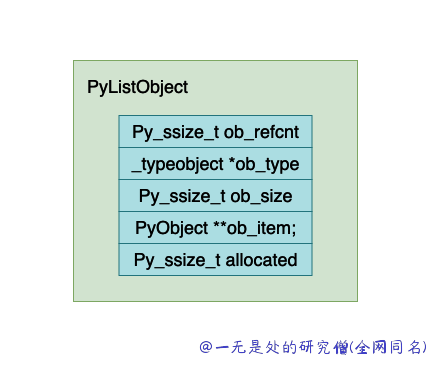
\includegraphics[scale=.5]{images/01-list.png}
            \caption{列表的字段结构}
        \label{fig:my_label}
    \end{figure}
    
现在来解释一下上面的各个字段的含义:
\begin{itemize}
\item Py\_ssize\_t,一个整型数据类型。 
\item ob\_refcnt,表示对象的引用记数的个数,这个对于垃圾回收很有用处,后面我们分析虚拟机中垃圾回收部分在深入分析。 
\item ob\_type,表示这个对象的数据类型是什么,在 python 当中有时候需要对数据的数据类型进行判断比如 isinstance, type 这两个关键字就会使用到这个字段。 
\item ob\_size,这个字段表示这个列表当中有多少个元素。 
\item ob\_item,这是一个指针,指向真正保存 python 对象数据的地址,大致的内存他们之间大致的内存布局如下所示: 

    \begin{figure}[h]
        \centering
            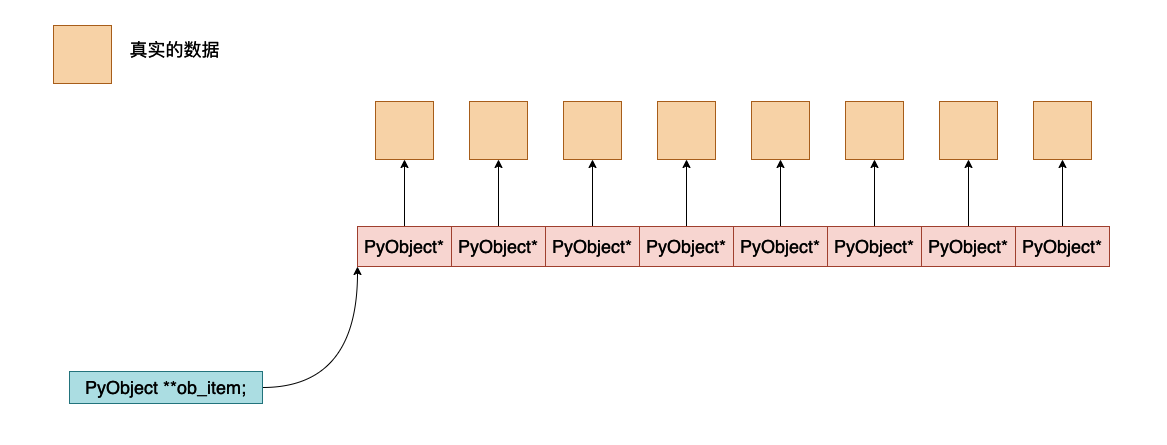
\includegraphics[scale=.3]{images/02-list.png}
        \caption{列表数据的内存大致布局}
        \label{fig:my_label}
    \end{figure}
    
\item allocated,这个表示在进行内存分配的时候,一共分配了多少个 (PyObject *) ,真实分配的内存空间为 `allocated * sizeof(PyObject *)`。 
\end{itemize}
\subsection{列表操作函数源代码分析}
\subsubsection{创建列表}
首先需要了解的是在 python 虚拟机内部为列表创建了一个数组,所有的创建的被释放的内存空间,并不会直接进行释放而是会将这些内存空间的首地址保存到这个数组当中,好让下一次申请创建新的列表的时候不需要再申请内存空间,而是直接将之前需要释放的内存直接进行复用即可。
\begin{lstlisting}[style=cpp,caption=, language=C++]

/* Empty list reuse scheme to save calls to malloc and free */
#ifndef PyList_MAXFREELIST
#define PyList_MAXFREELIST 80
#endif
static PyListObject *free_list[PyList_MAXFREELIST];
static int numfree = 0;
\end{lstlisting}
\begin{itemize}
\item free\_list,保存被释放的内存空间的首地址。 
\item numfree,目前 free\_list 当中有多少个地址是可以被使用的,事实上是 free\_list 前 numfree 个首地址是可以被使用的。 
\end{itemize}
创建链表的代码如下所示(为了精简删除了一些代码只保留核心部分):
\begin{lstlisting}[style=cpp,caption=, language=C++]

PyObject *
PyList_New(Py_ssize_t size)
{
    PyListObject *op;
    size_t nbytes;
    /* Check for overflow without an actual overflow,
     *  which can cause compiler to optimise out */
    if ((size_t)size > PY_SIZE_MAX / sizeof(PyObject *))
        return PyErr_NoMemory();
    nbytes = size * sizeof(PyObject *);
  // 如果 numfree 不等于 0 那么说明现在 free_list 有之前使用被释放的内存空间直接使用这部分即可
    if (numfree) {
        numfree--;
        op = free_list[numfree]; // 将对应的首地址返回
        _Py_NewReference((PyObject *)op); // 这条语句的含义是将 op 这个对象的 reference count 设置成 1
    } else {
      // 如果没有空闲的内存空间 那么就需要申请内存空间 这个函数也会对对象的 reference count 进行初始化 设置成 1
        op = PyObject_GC_New(PyListObject, &PyList_Type);
        if (op == NULL)
            return NULL;
    }
  /* 下面是申请列表对象当中的 ob_item 申请内存空间,上面只是给列表本身申请内存空间,但是列表当中有许多元素
  	保存这些元素也是需要内存空间的 下面便是给这些对象申请内存空间
  */
    if (size <= 0)
        op->ob_item = NULL;
    else {
        op->ob_item = (PyObject **) PyMem_MALLOC(nbytes);
      // 如果申请内存空间失败 则报错
        if (op->ob_item == NULL) {
            Py_DECREF(op);
            return PyErr_NoMemory();
        }
      // 对元素进行初始化操作 全部赋值成 0
        memset(op->ob_item, 0, nbytes);
    }
  // Py_SIZE 是一个宏
    Py_SIZE(op) = size; // 这条语句会被展开成 (PyVarObject*)(ob))->ob_size = size
  // 分配数组的元素个数是 size
    op->allocated = size;
  // 下面这条语句对于垃圾回收比较重要 主要作用就是将这个列表对象加入到垃圾回收的链表当中
  // 后面如果这个对象的 reference count 变成 0 或者其他情况 就可以进行垃圾回收了
    _PyObject_GC_TRACK(op);
    return (PyObject *) op;
}
\end{lstlisting}
在 cpython 当中,创建链表的字节码为 BUILD\_LIST,我们可以在文件 ceval.c 当中找到对应的字节码对应的执行步骤:
\begin{lstlisting}[style=cpp,caption=, language=C++]

TARGET(BUILD_LIST) {
    PyObject *list =  PyList_New(oparg);
    if (list == NULL)
        goto error;
    while (--oparg >= 0) {
        PyObject *item = POP();
        PyList_SET_ITEM(list, oparg, item);
    }
    PUSH(list);
    DISPATCH();
}
\end{lstlisting}
从上面 BUILD\_LIST 字节码对应的解释步骤可以知道,在解释执行字节码 BUILD\_LIST 的时候确实调用了函数 PyList\_New 创建一个新的列表。
\subsubsection{列表 append 函数}
\begin{lstlisting}[style=cpp,caption=, language=C++]

static PyObject *
// 这个函数的传入参数是列表本身 self 需要 append 的元素为 v
  // 也就是将对象 v 加入到列表 self 当中
listappend(PyListObject *self, PyObject *v)
{
    if (app1(self, v) == 0)
        Py_RETURN_NONE;
    return NULL;
}
static int
app1(PyListObject *self, PyObject *v)
{
  // PyList_GET_SIZE(self) 展开之后为 ((PyVarObject*)(self))->ob_size
    Py_ssize_t n = PyList_GET_SIZE(self);
    assert (v != NULL);
  // 如果元素的个数已经等于允许的最大的元素个数 就报错
    if (n == PY_SSIZE_T_MAX) {
        PyErr_SetString(PyExc_OverflowError,
            "cannot add more objects to list");
        return -1;
    }
	// 下面的函数 list_resize 会保存 ob_item 指向的位置能够容纳最少 n+1 个元素(PyObject *)
  // 如果容量不够就会进行扩容操作
    if (list_resize(self, n+1) == -1)
        return -1;
		
  // 将对象 v 的 reference count 加一 因为列表当中使用了一次这个对象 所以对象的引用计数需要进行加一操作
    Py_INCREF(v);
    PyList_SET_ITEM(self, n, v); // 宏展开之后 ((PyListObject *)(op))->ob_item[i] = v
    return 0;
}
\end{lstlisting}
\subsubsection{列表的扩容机制}
\begin{lstlisting}[style=cpp,caption=, language=C++]

static int
list_resize(PyListObject *self, Py_ssize_t newsize)
{
    PyObject **items;
    size_t new_allocated;
    Py_ssize_t allocated = self->allocated;
    /* Bypass realloc() when a previous overallocation is large enough
       to accommodate the newsize.  If the newsize falls lower than half
       the allocated size, then proceed with the realloc() to shrink the list.
    */
  // 如果列表已经分配的元素个数大于需求个数 newsize 的就直接返回不需要进行扩容
    if (allocated >= newsize && newsize >= (allocated >> 1)) {
        assert(self->ob_item != NULL || newsize == 0);
        Py_SIZE(self) = newsize;
        return 0;
    }
    /* This over-allocates proportional to the list size, making room
     * for additional growth.  The over-allocation is mild, but is
     * enough to give linear-time amortized behavior over a long
     * sequence of appends() in the presence of a poorly-performing
     * system realloc().
     * The growth pattern is:  0, 4, 8, 16, 25, 35, 46, 58, 72, 88, ...
     */
  // 这是核心的数组大小扩容机制 new_allocated 表示新增的数组大小
    new_allocated = (newsize >> 3) + (newsize < 9 ? 3 : 6);
    /* check for integer overflow */
    if (new_allocated > PY_SIZE_MAX _mmnewsize) { 
        PyErr_NoMemory();
        return -1;
    } else {
        new_allocated += newsize;
    }
    if (newsize == 0)
        new_allocated = 0;
    items = self->ob_item;
    if (new_allocated <= (PY_SIZE_MAX / sizeof(PyObject *)))
      	// PyMem_RESIZE 这是一个宏定义 会申请 new_allocated 个数元素并且将原来数组的元素拷贝到新的数组当中
        PyMem_RESIZE(items, PyObject *, new_allocated);
    else
        items = NULL;
  // 如果没有申请到内存 那么报错
    if (items == NULL) {
        PyErr_NoMemory();
        return -1;
    }
  // 更新列表当中的元素数据
    self->ob_item = items;
    Py_SIZE(self) = newsize;
    self->allocated = new_allocated;
    return 0;
}
\end{lstlisting}
在上面的扩容机制下,数组的大小变化大致如下所示:
$$
newsize \approx size \cdot (size + 1)^{\frac{1}{8}}
$$

    \begin{figure}[h]
        \centering
            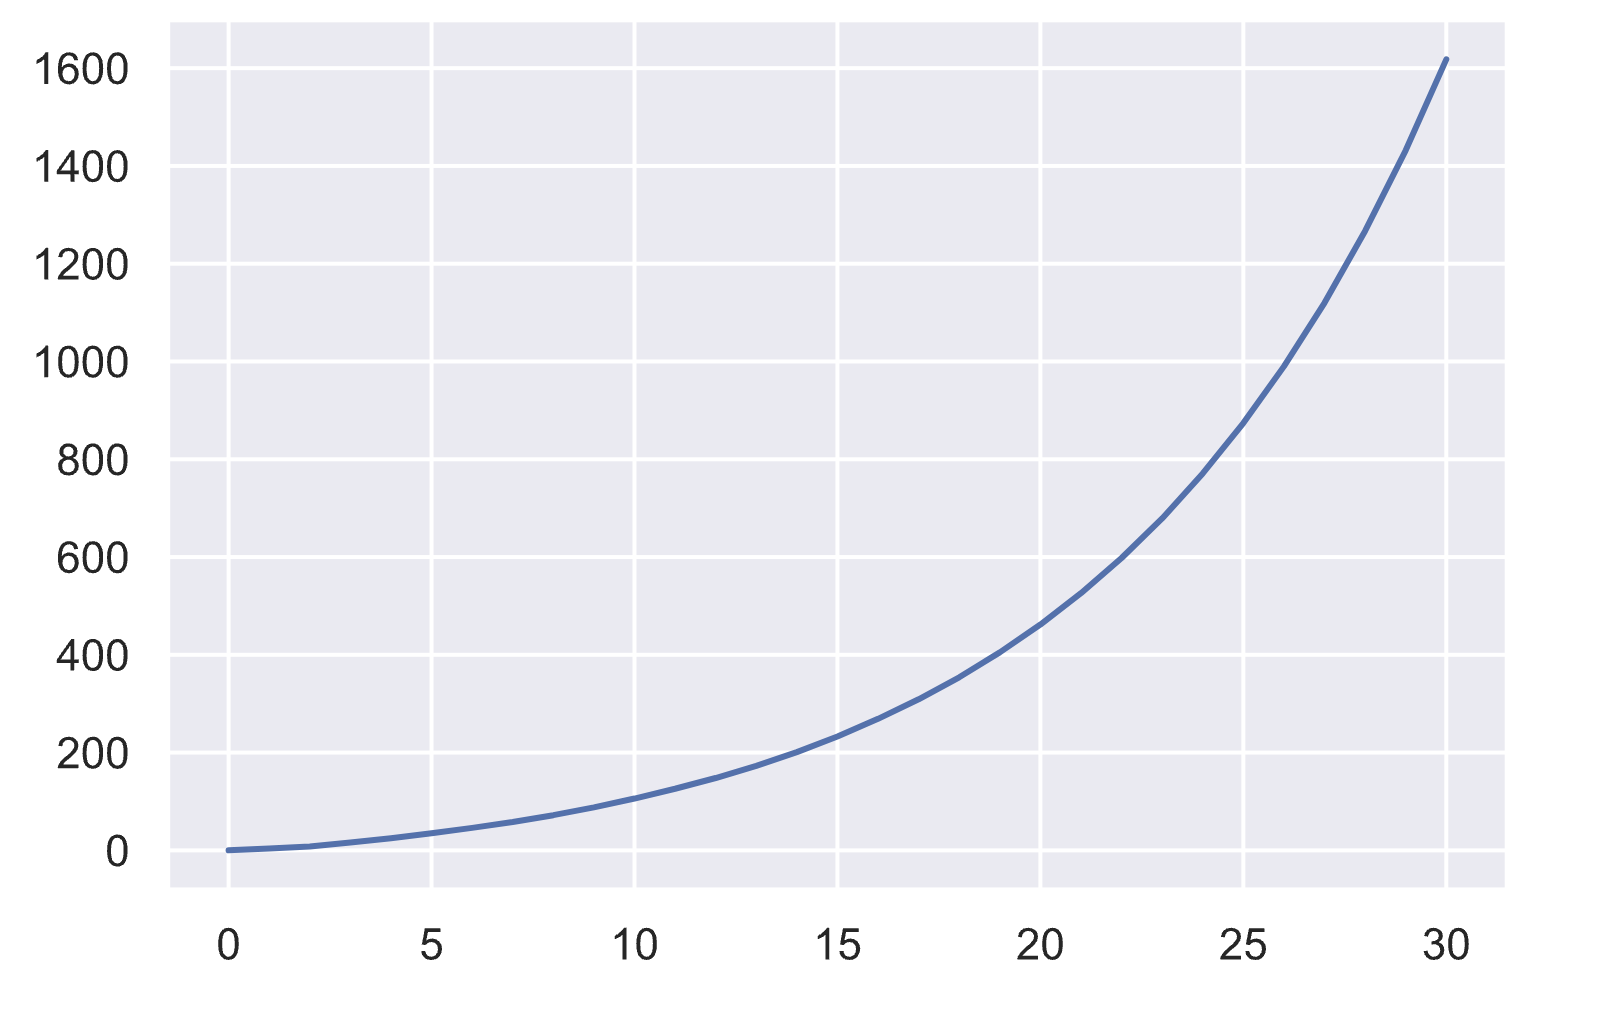
\includegraphics[scale=.2]{images/03-list.png}
            \caption{列表数据容量变化图}
        \label{fig:my_label}
    \end{figure}
    
\subsubsection{列表的插入函数 insert}
在列表当中插入一个数据比较简单,只需要将插入位置和其后面的元素往后移动一个位置即可,整个过程如下所示:

    \begin{figure}[h]
        \centering
            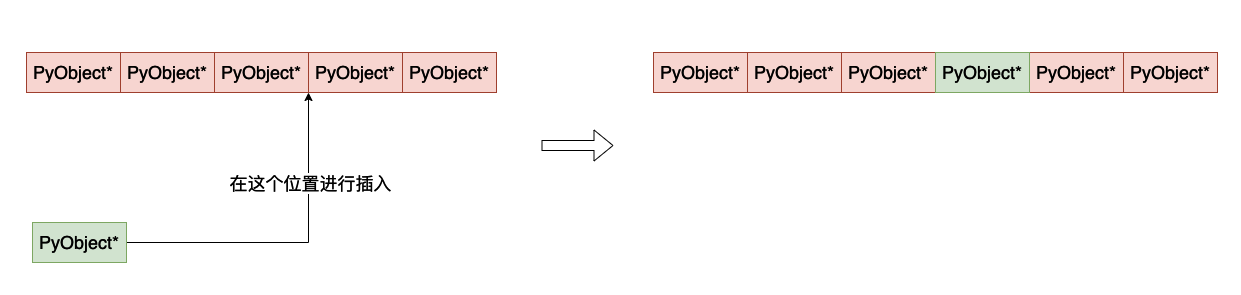
\includegraphics[scale=.3]{images/04-list.png}
            \caption{ }
        \label{fig:my_label}
    \end{figure}
    
在 cpython 当中列表的插入函数的实现如下所示:
\begin{itemize}
\item 参数 op 表示往哪个链表当中插入元素。 
\item 参数 where 表示在链表的哪个位置插入元素。 
\item 参数 newitem 表示新插入的元素。 
\end{itemize}
\begin{lstlisting}[style=cpp,caption=, language=C++]

int
PyList_Insert(PyObject *op, Py_ssize_t where, PyObject *newitem)
{
  // 检查是否是列表类型
    if (!PyList_Check(op)) {
        PyErr_BadInternalCall();
        return -1;
    }
  // 如果是列表类型则进行插入操作
    return ins1((PyListObject *)op, where, newitem);
}
static int
ins1(PyListObject *self, Py_ssize_t where, PyObject *v)
{
    Py_ssize_t i, n = Py_SIZE(self);
    PyObject **items;
    if (v == NULL) {
        PyErr_BadInternalCall();
        return -1;
    }
  // 如果列表的元素个数超过限制 则进行报错
    if (n == PY_SSIZE_T_MAX) {
        PyErr_SetString(PyExc_OverflowError,
            "cannot add more objects to list");
        return -1;
    }
  // 确保列表能够容纳 n + 1 个元素
    if (list_resize(self, n+1) == -1)
        return -1;
  // 这里是 python 的一个小 trick 就是下标能够有负数的原理
    if (where < 0) {
        where += n;
        if (where < 0)
            where = 0;
    }
    if (where > n)
        where = n;
    items = self->ob_item;
  // 从后往前进行元素的拷贝操作,也就是将插入位置及其之后的元素往后移动一个位置
    for (i = n; --i >= where; )
        items[i+1] = items[i];
  // 因为链表应用的对象,因此对象的 reference count 需要进行加一操作
    Py_INCREF(v);
  // 在列表当中保存对象 v 
    items[where] = v;
    return 0;
}
\end{lstlisting}
\subsubsection{列表的删除函数 remove}
对于数组 ob\_item 来说,删除一个元素就需要将这个元素后面的元素往前移动,因此整个过程如下所示:

    \begin{figure}[h]
        \centering
            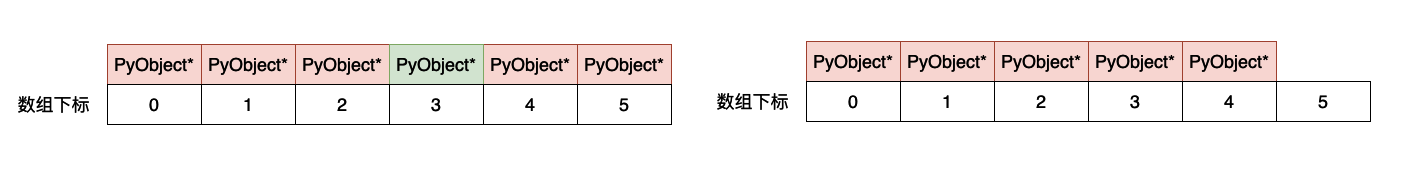
\includegraphics[scale=.3]{images/05-list.png}
            \caption{ }
        \label{fig:my_label}
    \end{figure}
    
\begin{lstlisting}[style=cpp,caption=cpython/objects/list.c, language=C++]

static PyObject *
listremove(PyListObject *self, PyObject *v)
{
    Py_ssize_t i;
  	// 编译数组 ob_item 查找和对象 v 相等的元素并且将其删除
    for (i = 0; i < Py_SIZE(self); i++) {
        int cmp = PyObject_RichCompareBool(self->ob_item[i], v, Py_EQ);
        if (cmp > 0) {
            if (list_ass_slice(self, i, i+1,
                               (PyObject *)NULL) == 0)
                Py_RETURN_NONE;
            return NULL;
        }
        else if (cmp < 0)
            return NULL;
    }
  	// 如果没有找到这个元素就进行报错处理 在下面有一个例子重新编译 python 解释器 将这个错误内容修改的例子
    PyErr_SetString(PyExc_ValueError, "list.remove(x): x not in list");
    return NULL;
}
\end{lstlisting}
执行的 python 程序内容为:
\begin{lstlisting}[style=py,caption=, language=Python]

data = []
data.remove(1)
\end{lstlisting}
下面是整个修改内容和报错结果:

    \begin{figure}[h]
        \centering
            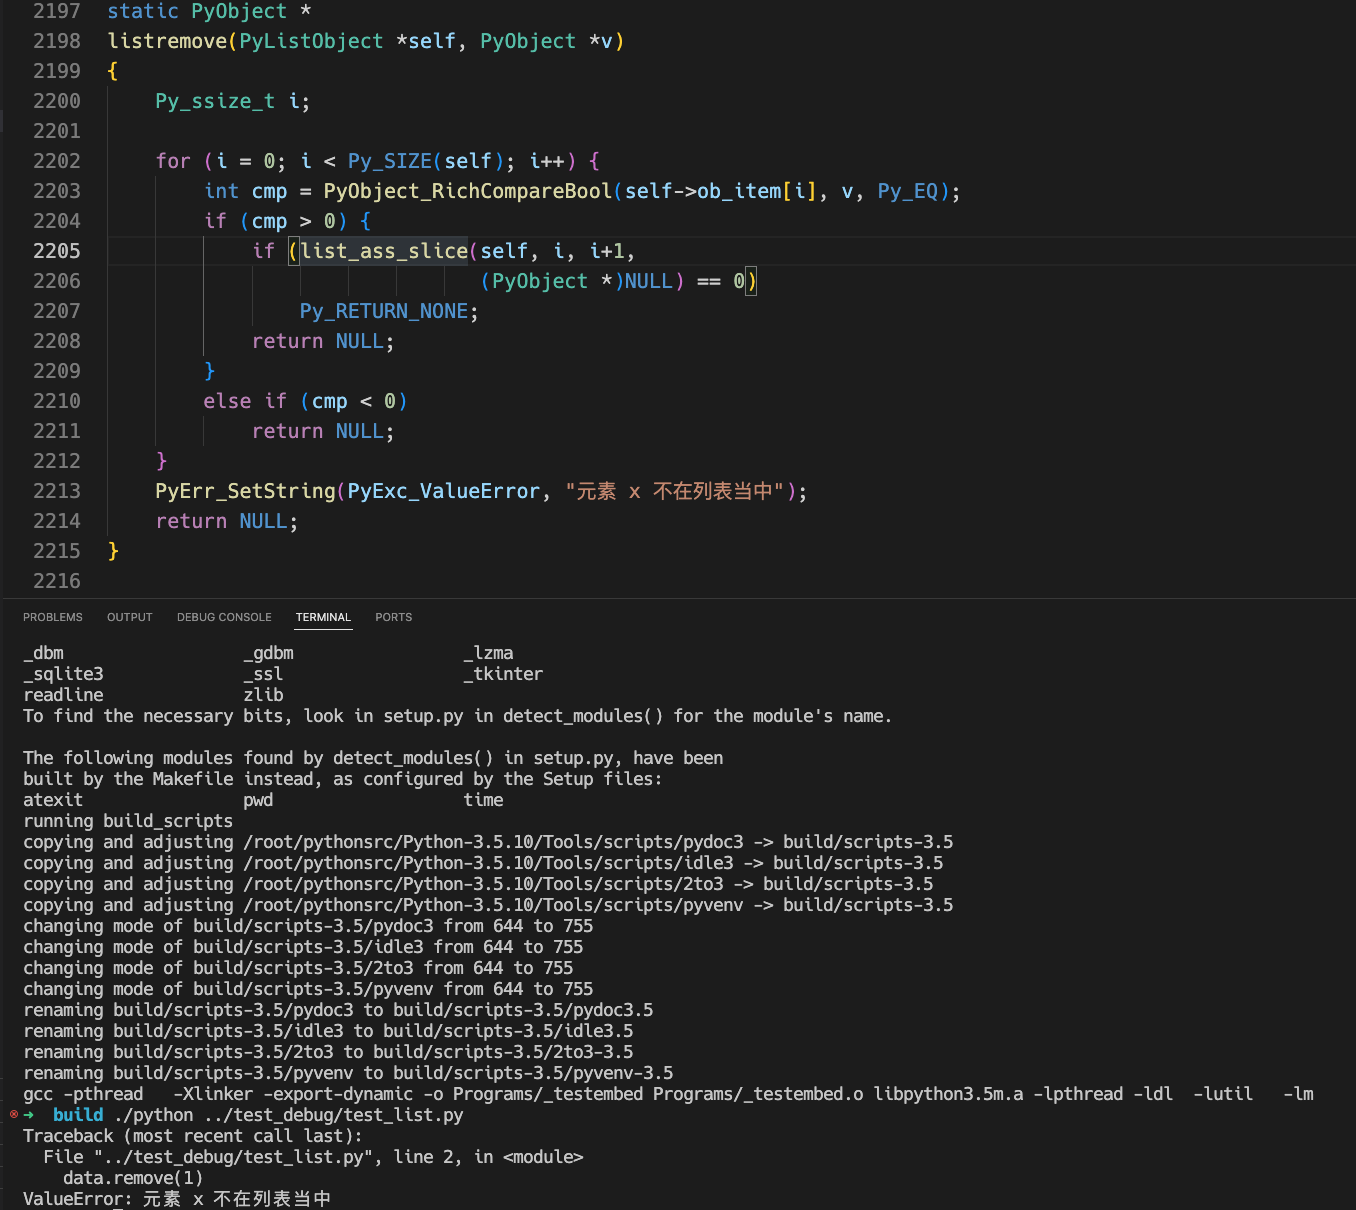
\includegraphics[scale=.2]{images/06-list.png}
            \caption{ }
        \label{fig:my_label}
    \end{figure}
    
从上面的结果我们可以看到的是,我们修改的错误信息正确打印了出来。
\subsubsection{列表的统计函数 count}
这个函数的主要作用就是统计列表 self 当中有多少个元素和 v 相等。
\begin{lstlisting}[style=cpp,caption=, language=C++]

static PyObject *
listcount(PyListObject *self, PyObject *v)
{
    Py_ssize_t count = 0;
    Py_ssize_t i;
    for (i = 0; i < Py_SIZE(self); i++) {
        int cmp = PyObject_RichCompareBool(self->ob_item[i], v, Py_EQ);
      // 如果相等则将 count 进行加一操作
        if (cmp > 0)
            count++;
      // 如果出现错误就返回 NULL
        else if (cmp < 0)
            return NULL;
    }
  // 将一个 Py_ssize_t 的变量变成 python 当中的对象
    return PyLong_FromSsize_t(count);
}
\end{lstlisting}
\subsubsection{列表的拷贝函数 copy}
这是列表的浅拷贝函数,它只拷贝了真实 python 对象的指针,并没有拷贝真实的 python 对象 ,从下面的代码可以知道列表的拷贝是浅拷贝,当 b 对列表当中的元素进行修改时,列表 a 当中的元素也改变了。如果需要进行深拷贝可以使用 copy 模块当中的 deepcopy 函数。
\begin{lstlisting}[style=py,caption=, language=Python]

>>> a = [1, 2, [3, 4]]
>>> b = a.copy()
>>> b[2][1] = 5
>>> b
[1, 2, [3, 5]]
\end{lstlisting}
copy 函数对应的源代码(listcopy)如下所示:
\begin{lstlisting}[style=cpp,caption=, language=C++]

static PyObject *
listcopy(PyListObject *self)
{
    return list_slice(self, 0, Py_SIZE(self));
}
static PyObject *
list_slice(PyListObject *a, Py_ssize_t ilow, Py_ssize_t ihigh)
{
  // Py_SIZE(a) 返回列表 a 当中元素的个数(注意不是数组的长度 allocated)
    PyListObject *np;
    PyObject **src, **dest;
    Py_ssize_t i, len;
    if (ilow < 0)
        ilow = 0;
    else if (ilow > Py_SIZE(a))
        ilow = Py_SIZE(a);
    if (ihigh < ilow)
        ihigh = ilow;
    else if (ihigh > Py_SIZE(a))
        ihigh = Py_SIZE(a);
    len = ihigh _mmilow; 
    np = (PyListObject *) PyList_New(len);
    if (np == NULL)
        return NULL;
    src = a->ob_item + ilow;
    dest = np->ob_item;
  // 可以看到这里循环拷贝的是指向真实 python 对象的指针 并不是真实的对象
    for (i = 0; i < len; i++) {
        PyObject *v = src[i];
      // 同样的因为并没有创建新的对象,但是这个对象被新的列表使用到啦 因此他的 reference count 需要进行加一操作 Py_INCREF(v) 的作用:将对象 v 的 reference count 加一
        Py_INCREF(v);
        dest[i] = v;
    }
    return (PyObject *)np;
}
\end{lstlisting}
下图就是使用 a.copy() 浅拷贝的时候,内存的布局的示意图,可以看到列表指向的对象数组发生了变化,但是数组中元素指向的 python 对象并没有发生变化。

    \begin{figure}[h]
        \centering
            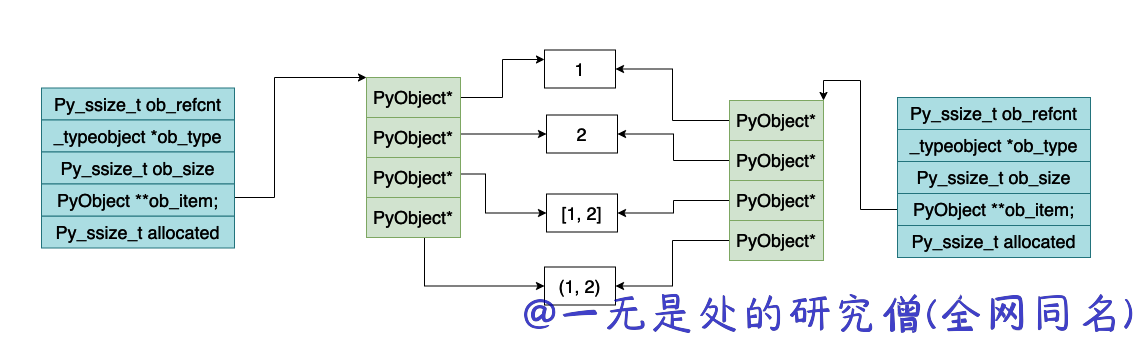
\includegraphics[scale=.3]{images/07-list.png}
            \caption{ }
        \label{fig:my_label}
    \end{figure}
    
下面是对列表对象进行深拷贝的时候内存的大致示意图,可以看到数组指向的 python 对象也是不一样的。

    \begin{figure}[h]
        \centering
            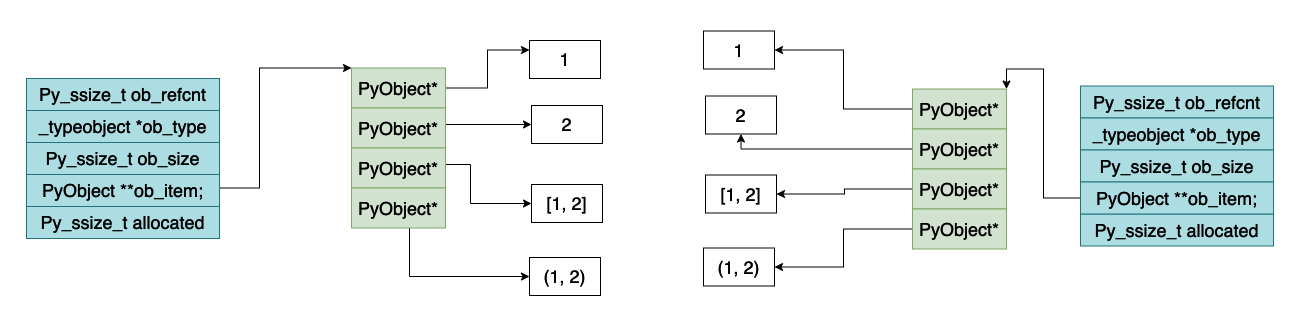
\includegraphics[scale=.3]{images/08-list.png}
            \caption{ }
        \label{fig:my_label}
    \end{figure}
    
\subsubsection{列表的清空函数 clear}
当我们在使用 list.clear() 的时候会调用下面这个函数。清空列表需要注意的就是将表示列表当中元素个数的 ob\_size 字段设置成 0 ,同时将列表当中所有的对象的 reference count 设置进行 -1 操作,这个操作是通过宏 Py\_XDECREF 实现的,这个宏还会做另外一件事就是如果这个对象的引用计数变成 0 了,那么就会直接释放他的内存。
\begin{lstlisting}[style=cpp,caption=, language=C++]

static PyObject *
listclear(PyListObject *self)
{
    list_clear(self);
    Py_RETURN_NONE;
}
static int
list_clear(PyListObject *a)
{
    Py_ssize_t i;
    PyObject **item = a->ob_item;
    if (item != NULL) {
        /* Because XDECREF can recursively invoke operations on
           this list, we make it empty first. */
        i = Py_SIZE(a);
        Py_SIZE(a) = 0;
        a->ob_item = NULL;
        a->allocated = 0;
        while (--i >= 0) {
            Py_XDECREF(item[i]);
        }
        PyMem_FREE(item);
    }
    /* Never fails; the return value can be ignored.
       Note that there is no guarantee that the list is actually empty
       at this point, because XDECREF may have populated it again! */
    return 0;
}
\end{lstlisting}
\subsubsection{列表反转函数 reverse}
在 python 当中如果我们想要反转类表当中的内容的话,就会使用这个函数 reverse 。
\begin{lstlisting}[style=py,caption=, language=Python]

>>> a = [i for i in range(10)]
>>> a.reverse()
>>> a
[9, 8, 7, 6, 5, 4, 3, 2, 1, 0]
\end{lstlisting}
其对应的源程序如下所示:
\begin{lstlisting}[style=cpp,caption=, language=C++]

static PyObject *
listreverse(PyListObject *self)
{
    if (Py_SIZE(self) > 1)
        reverse_slice(self->ob_item, self->ob_item + Py_SIZE(self));
    Py_RETURN_NONE;
}
static void
reverse_slice(PyObject **lo, PyObject **hi)
{
    assert(lo && hi);
    --hi;
    while (lo < hi) {
        PyObject *t = *lo;
        *lo = *hi;
        *hi = t;
        ++lo;
        --hi;
    }
}
\end{lstlisting}
上面的源程序还是比较容易理解的,给 reverse\_slice 传递的参数就是保存数据的数组的首尾地址,然后不断的将首尾数据进行交换(其实是交换指针指向的地址)。
\subsection{总结}
本文介绍了 Python 中列表对象的实现细节,介绍了一些常用函数的实现,包括列表的扩容机制,插入、删除、统计、拷贝、清空和反转等操作的实现方式。
\begin{itemize}
\item 列表的扩容机制采用了一种线性时间摊销的方式,使得列表的插入操作具有较好的时间复杂度。 
\item 列表的插入、删除和统计操作都是通过操作ob\_item 数组实现的,其中插入和删除操作需要移动数组中的元素。 
\item 列表的拷贝操作是浅拷贝,需要注意的是进行深拷贝需要使用 copy 模块当中的 deepcopy 函数。 
\item 列表清空会将 ob\_size 字段设置成 0,同时需要将列表当中的所有对象的 reference count 进行 -1 操作,从而避免内存泄漏。 
\item 列表的反转操作可以通过交换 ob\_item 数组中前后元素的位置实现。 
\end{itemize}
总之,了解 Python 列表对象的实现细节有助于我们更好地理解 Python 的内部机制,从而编写更高效、更可靠的 Python 代码。

\section{元组(tuple)的实现原理及源码剖析}
在本小节当中主要给大家介绍 cpython 虚拟机当中针对列表的实现,在 Python 中,tuple 是一种非常常用的数据类型,在本小节当中将深入去分析这一点是如何实现的。
\subsection{元组的结构}
在这一小节当中主要介绍在 python 当中元组的数据结构:
\begin{lstlisting}[style=cpp,caption=, language=C++]

typedef struct {
    PyObject_VAR_HEAD
    PyObject *ob_item[1];
    /* ob_item contains space for 'ob_size' elements.
     * Items must normally not be NULL, except during construction when
     * the tuple is not yet visible outside the function that builds it.
     */
} PyTupleObject;
#define PyObject_VAR_HEAD      PyVarObject ob_base;
typedef struct {
    PyObject ob_base;
    Py_ssize_t ob_size; /* Number of items in variable part */
} PyVarObject;
typedef struct _object {
    _PyObject_HEAD_EXTRA
    Py_ssize_t ob_refcnt;
    struct _typeobject *ob_type;
} PyObject;
\end{lstlisting}
从上面的数据结构来看和 list 的数据结构基本上差不多,最终的使用方法也差不多。将上面的结构体展开之后,PyTupleObject 的结构大致如下所示:

    \begin{figure}[h]
        \centering
            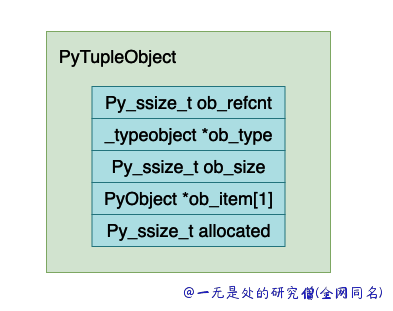
\includegraphics[scale=.5]{images/09-tuple.png}
            \caption{ }
        \label{fig:my_label}
    \end{figure}
    
现在来解释一下上面的各个字段的含义:
\begin{itemize}
\item Py\_ssize\_t,一个整型数据类型。 
\item ob\_refcnt,表示对象的引用记数的个数,这个对于垃圾回收很有用处,后面我们分析虚拟机中垃圾回收部分在深入分析。 
\item ob\_type,表示这个对象的数据类型是什么,在 python 当中有时候需要对数据的数据类型进行判断比如 isinstance, type 这两个关键字就会使用到这个字段。 
\item ob\_size,这个字段表示这个元组当中有多少个元素。 
\item ob\_item,这是一个指针,指向真正保存 python 对象数据的地址,大致的内存他们之间大致的内存布局如下所示: 

    \begin{figure}[h]
        \centering
            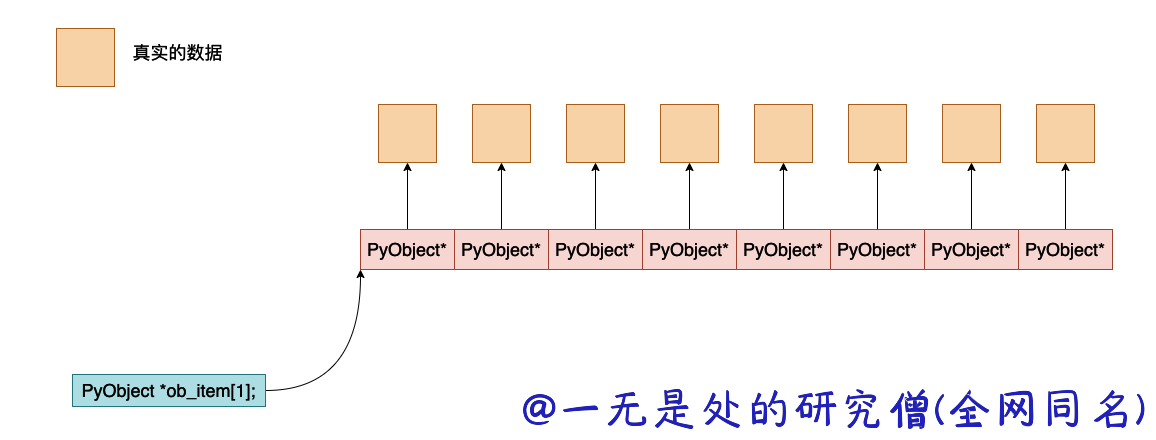
\includegraphics[scale=.3]{images/10-tuple.png}
            \caption{ }
        \label{fig:my_label}
    \end{figure}
    
\end{itemize}
需要注意的是元组的数组大小是不能够进行更改的,这一点和 list 不一样,我们可以注意到在 list 的数据结构当中还有一个 allocated 字段,但是在元组当中是没有的,这主要是因为元组的数组大小是固定的,而列表的数组大小是可以更改的。
\subsection{元组操作函数源码剖析}
\subsubsection{创建元组}
首先我们需要了解一下在 cpython 内部关于元组内存分配的问题,首先和 list 一样,在 cpython 当中对于分配的好的元组进行释放的时候,并不会直接进行释放,而是会先保存下来,当下次又有元组申请内存的时候,直接将这块内存进行返回即可。
在 cpython 内部会进行缓存的元组大小为 20,如果元组的长度为 0 - 19 那么在申请分配内存之后释放并不会直接释放,而是将其先保存下来,下次有需求的时候直接分配,而不需要申请。在 cpython 内部,相关的定义如下所示:
\begin{lstlisting}[style=cpp,caption=, language=C++]

static PyTupleObject *free_list[PyTuple_MAXSAVESIZE];
static int numfree[PyTuple_MAXSAVESIZE];
\end{lstlisting}
\begin{itemize}
\item free\_list,保存指针——指向被释放的元组。 
\item numfree,对应的下标表示元组当中元素的个数,numfree[i] 表示有 i 个元素的元组的个数。 
\end{itemize}
下面是新建 tuple 对象的源程序:
\begin{lstlisting}[style=cpp,caption=, language=C++]

PyObject *
PyTuple_New(Py_ssize_t size)
{
    PyTupleObject *op;
    Py_ssize_t i;
    if (size < 0) {
        PyErr_BadInternalCall();
        return NULL;
    }
#if PyTuple_MAXSAVESIZE > 0
    // 如果申请一个空的元组对象 当前的 free_list 当中是否存在空元组对象 如果存在则直接返回
    if (size == 0 && free_list[0]) k
        op = free_list[0];
        Py_INCREF(op);
        return (PyObject *) op;
    }
    // 如果元组的对象元素个数小于 20 而且对应的 free_list 当中还有余下的元组对象 则不需要进行内存申请直接返回
    if (size < PyTuple_MAXSAVESIZE && (op = free_list[size]) != NULL) {
        free_list[size] = (PyTupleObject *) op->ob_item[0];
        numfree[size]--;
        /* Inline PyObject_InitVar */
        _Py_NewReference((PyObject *)op); // _Py_NewReference 这个宏是将对象 op 的引用计数设置成 1
    }
    else
#endif
    {
        /* Check for overflow */
        // 如果元组的元素个数大或者等于 20 或者 当前 free_list 当中没有没有剩余的对象则需要进行内存申请
        if ((size_t)size > ((size_t)PY_SSIZE_T_MAX _mmsizeof(PyTupleObject) - 
                    sizeof(PyObject *)) / sizeof(PyObject *)) {
          	// 如果元组长度大于某个值直接报内存错误
            return PyErr_NoMemory();
        }
        // 申请元组大小的内存空间
        op = PyObject_GC_NewVar(PyTupleObject, &PyTuple_Type, size);
        if (op == NULL)
            return NULL;
    }
		// 初始化内存空间
    for (i=0; i < size; i++)
        op->ob_item[i] = NULL;
#if PyTuple_MAXSAVESIZE > 0
    // 因为 size == 0 的元组不会进行修改操作 因此可以直接将这个申请到的对象放到 free_list 当中以备后续使用
    if (size == 0) {
        free_list[0] = op;
        ++numfree[0];
        Py_INCREF(op);          /* extra INCREF so that this is never freed */
    }
#endif
    _PyObject_GC_TRACK(op); // _PyObject_GC_TRACK 这个宏是将对象 op 将入到垃圾回收队列当中
    return (PyObject *) op;
}
\end{lstlisting}
新建元组对象的流程如下所示:
\begin{itemize}
\item 查看 free\_list 当中是否已经存在空闲的元组,如果有则直接进行返回。 
\item 如果没有,则进行内存分配,然后将申请的内存空间进行初始化操作。 
\item 如果 size == 0,则可以将新分配的元组对象放到 free\_list 当中。 
\end{itemize}
\subsubsection{查看元组的长度}
这个功能比较简单,直接只用 cpython 当中的宏 Py\_SIZE 即可。他的宏定义为 \#define Py\_SIZE(ob) (((PyVarObject*)(ob))->ob\_size)。
\begin{lstlisting}[style=cpp,caption=, language=C++]

static Py_ssize_t
tuplelength(PyTupleObject *a)
{
    return Py_SIZE(a);
}
\end{lstlisting}
\subsubsection{元组当中是否包含数据}
这个其实和 list 一样,就是遍历元组当中的数据,然后进行比较即可。
\begin{lstlisting}[style=cpp,caption=, language=C++]

static int
tuplecontains(PyTupleObject *a, PyObject *el)
{
    Py_ssize_t i;
    int cmp;
    for (i = 0, cmp = 0 ; cmp == 0 && i < Py_SIZE(a); ++i)
        cmp = PyObject_RichCompareBool(el, PyTuple_GET_ITEM(a, i),
                                           Py_EQ);
    return cmp;
}
\end{lstlisting}
\subsubsection{获取和设置元组中的数据}
这两个方法也比较简单,首先检查数据类型是不是元组类型,然后判断是否越界,之后就返回数据,或者设置对应的数据。
这里在设置数据数据的时候需要注意一点的是,当设置新的数据的时候,原来的 python 对象引用计数需要减去一,同理如果设置没有成功的话传入的新的数据的引用计数也需要减去一。
\begin{lstlisting}[style=cpp,caption=, language=C++]

PyObject *
PyTuple_GetItem(PyObject *op, Py_ssize_t i)
{
    if (!PyTuple_Check(op)) {
        PyErr_BadInternalCall();
        return NULL;
    }
    if (i < 0 || i >= Py_SIZE(op)) {
        PyErr_SetString(PyExc_IndexError, "tuple index out of range");
        return NULL;
    }
    return ((PyTupleObject *)op) -> ob_item[i];
}
int
PyTuple_SetItem(PyObject *op, Py_ssize_t i, PyObject *newitem)
{
    PyObject *olditem;
    PyObject **p;
    if (!PyTuple_Check(op) || op->ob_refcnt != 1) {
        Py_XDECREF(newitem);
        PyErr_BadInternalCall();
        return -1;
    }
    if (i < 0 || i >= Py_SIZE(op)) {
        Py_XDECREF(newitem);
        PyErr_SetString(PyExc_IndexError,
                        "tuple assignment index out of range");
        return -1;
    }
    p = ((PyTupleObject *)op) -> ob_item + i;
    olditem = *p;
    *p = newitem;
    Py_XDECREF(olditem);
    return 0;
}
\end{lstlisting}
\subsubsection{释放元组内存空间}
当我们在进行垃圾回收的时候,判定一个对象的引用计数等于 0 的时候就需要释放这块内存空间(相当于析构函数),下面就是释放 tuple 内存空间的函数。
\begin{lstlisting}[style=cpp,caption=, language=C++]

static void
tupledealloc(PyTupleObject *op)
{
    Py_ssize_t i;
    Py_ssize_t len =  Py_SIZE(op);
    PyObject_GC_UnTrack(op); // PyObject_GC_UnTrack 将对象从垃圾回收队列当中移除
    Py_TRASHCAN_SAFE_BEGIN(op) 
    if (len > 0) {
        i = len;
        while (--i >= 0)
            // 将这个元组指向的对象的引用计数减去一
            Py_XDECREF(op->ob_item[i]);
#if PyTuple_MAXSAVESIZE > 0
        // 如果这个元组对象满足加入 free_list  的条件,则将这个元组对象加入到 free_list 当中
        if (len < PyTuple_MAXSAVESIZE &&
            numfree[len] < PyTuple_MAXFREELIST &&
            Py_TYPE(op) == &PyTuple_Type)
        {
            op->ob_item[0] = (PyObject *) free_list[len];
            numfree[len]++;
            free_list[len] = op;
            goto done; /* return */
        }
#endif
    }
    Py_TYPE(op)->tp_free((PyObject *)op);
done:
    Py_TRASHCAN_SAFE_END(op)
}
\end{lstlisting}
将元组的内存空间回收的时候,主要有以下几个步骤:
\begin{itemize}
\item 将元组对象从垃圾回收链表当中移除。 
\item 将元组指向的所有对象的引用计数减一。 
\item 判断元组是否满足保存到 free\_list 当中的条件,如果满足就将他加入到 free\_list 当中去,否则回收这块内存。加入到 free\_list 当中整个元组当中 ob\_item 指向变化如下所示: 

    \begin{figure}[h]
        \centering
            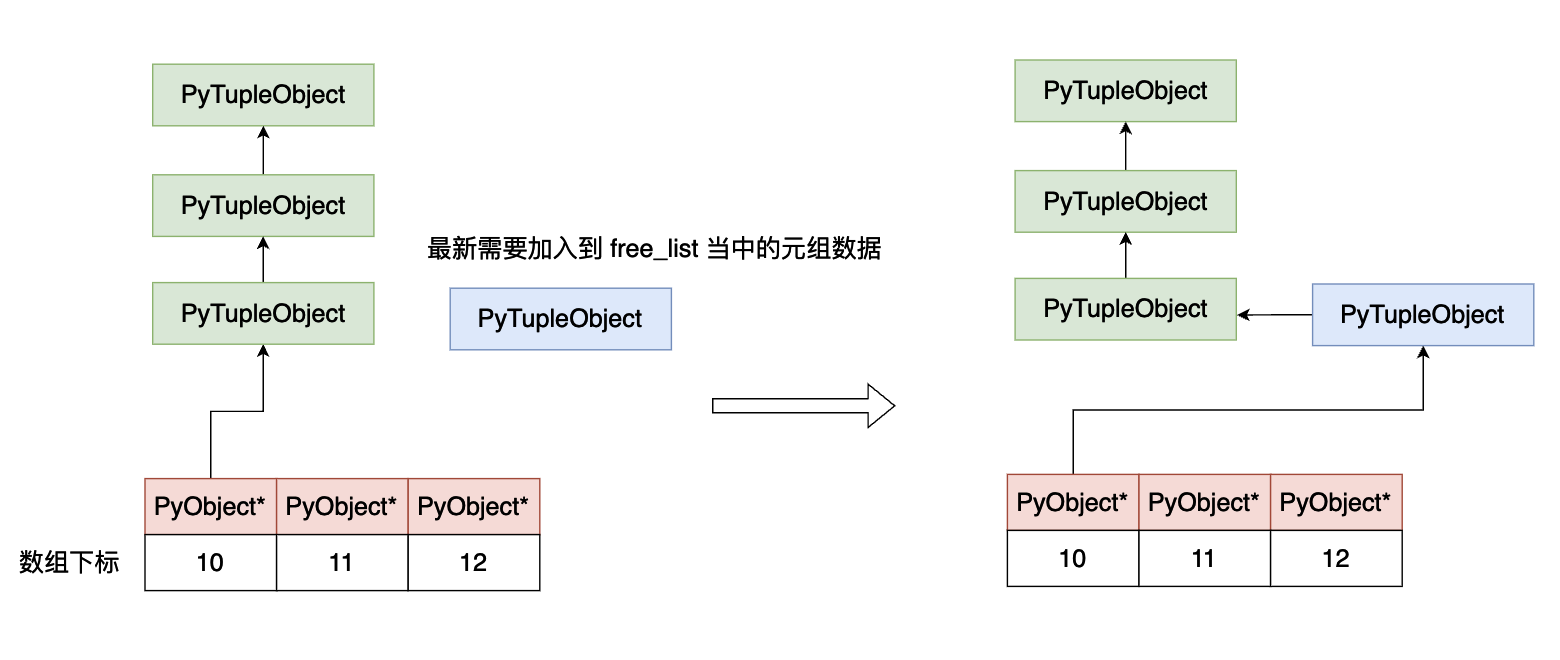
\includegraphics[scale=.2]{images/11-tuple.png}
            \caption{ }
        \label{fig:my_label}
    \end{figure}
    
\item 如果不能够将释放的元组对象加入到 free\_list 当中,否则将内存释放回收。 
\end{itemize}
\subsection{总结}
在本小节当中主要介绍了在 cpython 当中是如何实现 tuple 的,以及相关的数据结构和一些基本的使用函数,最后简单谈了关于元组内存释放的问题,这里面还是涉及一些其他的知识点,不能够在这篇文章进行分析,在本文内存分配主要是聚焦在元组身上,主要是分析内存分配和 tuple 的 free\_list 是如何交互的。


\section{字典(dict)的实现原理及源码剖析}
在本小节当中主要给大家深入介绍一下在 cpython 当中字典的实现原理,在本小节当中主要介绍在早期 python3 当中的版本字典的实现,现在的字典做了部分优化,我们在后面的文章当中再介绍。
\subsection{字典数据结构分析}
\begin{lstlisting}[style=cpp,caption=, language=C++]

/* The ma_values pointer is NULL for a combined table
 * or points to an array of PyObject* for a split table
 */
typedef struct {
    PyObject_HEAD
    Py_ssize_t ma_used;
    PyDictKeysObject *ma_keys;
    PyObject **ma_values;
} PyDictObject;
struct _dictkeysobject {
    Py_ssize_t dk_refcnt;
    Py_ssize_t dk_size;
    dict_lookup_func dk_lookup;
    Py_ssize_t dk_usable;
    PyDictKeyEntry dk_entries[1];
};
typedef struct {
    /* Cached hash code of me_key. */
    Py_hash_t me_hash;
    PyObject *me_key;
    PyObject *me_value; /* This field is only meaningful for combined tables */
} PyDictKeyEntry;
\end{lstlisting}

    \begin{figure}[h]
        \centering
            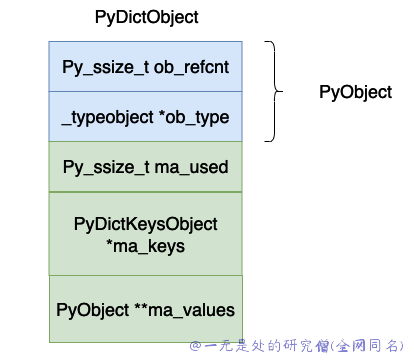
\includegraphics[scale=.3]{images/26-dict.png}
            \caption{ }
        \label{fig:my_label}
    \end{figure}
    
上面的各个字段的含义为:
\begin{itemize}
\item ob\_refcnt,对象的引用计数。 
\item ob\_type,对象的数据类型。 
\item ma\_used,当前哈希表当中的数据个数。 
\item ma\_keys,指向保存键值对的数组。 
\item ma\_values,这个指向值的数组,但是在 cpython 的具体实现当中不一定使用这个值,因为 \_dictkeysobject 当中的 PyDictKeyEntry 数组当中的对象也是可以存储 value 的,这个值只有在键全部是字符串的时候才可能会使用,在本小节当中主要使用 PyDictKeyEntry 当中的 value 来讨论字典的实现,因此大家可以忽略这个变量。 
\item dk\_refcnt,这个也是用于表示引用计数,这个跟字典的视图有关系,原理和引用计数类似,这里暂时不管。 
\item dk\_size,这个表示哈希表的大小,必须是 $2^n$,这样的话可以将模运算变成位与运算。 
\item dk\_lookup,这个表示哈希表的查找函数,他是一个函数指针。 
\item dk\_usable,表示当前数组当中还有多少个可以使用的键值对。 
\item dk\_entries,哈希表,真正存储键值对的地方。 
\end{itemize}
整个哈希表的布局大致如下图所示:

    \begin{figure}[h]
        \centering
            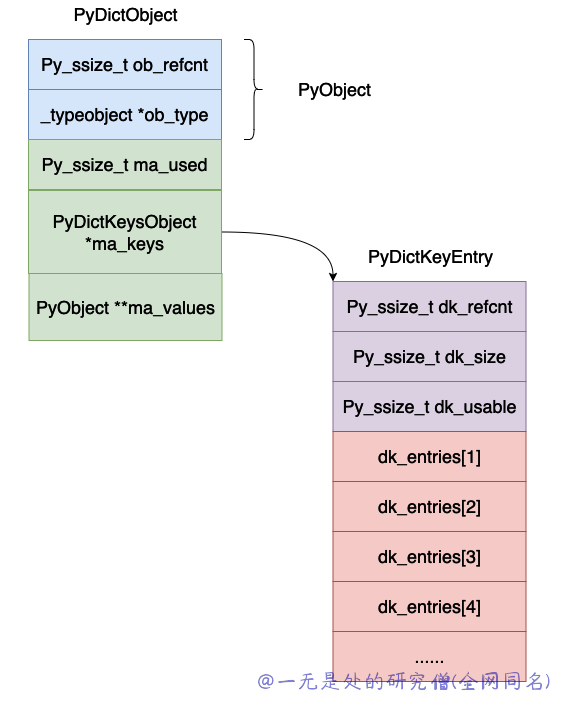
\includegraphics[scale=.25]{images/27-dict.png}
            \caption{ }
        \label{fig:my_label}
    \end{figure}
    
\subsection{创建新字典对象}
这个函数还是比较简单,首先申请内存空间,然后进行一些初始化操作,申请哈希表用于保存键值对。
\begin{lstlisting}[style=cpp,caption=, language=C++]

static PyObject *
dict_new(PyTypeObject *type, PyObject *args, PyObject *kwds)
{
    PyObject *self;
    PyDictObject *d;
    assert(type != NULL && type->tp_alloc != NULL);
    // 申请内存空间
    self = type->tp_alloc(type, 0);
    if (self == NULL)
        return NULL;
    d = (PyDictObject *)self;
    /* The object has been implicitly tracked by tp_alloc */
    if (type == &PyDict_Type)
        _PyObject_GC_UNTRACK(d);
    // 因为还没有增加数据 因此哈希表当中 ma_used = 0
    d->ma_used = 0;
    // 申请保存键值对的数组  PyDict_MINSIZE_COMBINED 是一个宏定义 值为 8 表示哈希表数组的最小长度
    d->ma_keys = new_keys_object(PyDict_MINSIZE_COMBINED);
    // 如果申请失败返回 NULL
    if (d->ma_keys == NULL) {
        Py_DECREF(self);
        return NULL;
    }
    return self;
}
// new_keys_object 函数如下所示
static PyDictKeysObject *new_keys_object(Py_ssize_t size)
{
    PyDictKeysObject *dk;
    Py_ssize_t i;
    PyDictKeyEntry *ep0;
    assert(size >= PyDict_MINSIZE_SPLIT);
    assert(IS_POWER_OF_2(size));
    // 这里是申请内存的位置真正申请内存空间的大小为 PyDictKeysObject 的大小加上 size-1 个PyDictKeyEntry的大小
    // 这里你可能会有一位为啥不是 size 个 PyDictKeyEntry 的大小 因为在结构体 PyDictKeysObject 当中已经申请了一个 PyDictKeyEntry 对象了
    dk = PyMem_MALLOC(sizeof(PyDictKeysObject) +
                      sizeof(PyDictKeyEntry) * (size-1));
    if (dk == NULL) {
        PyErr_NoMemory();
        return NULL;
    }
    // 下面主要是一些初始化的操作 dk_refcnt 设置成 1 因为目前只有一个字典对象使用 这个 PyDictKeysObject 对象
    DK_DEBUG_INCREF dk->dk_refcnt = 1;
    dk->dk_size = size; // 哈希表的大小
    // 下面这行代码主要是表示哈希表当中目前还能存储多少个键值对 在 cpython 的实现当中允许有 2/3 的数组空间去存储数据 超过这个数则需要进行扩容
    dk->dk_usable = USABLE_FRACTION(size); // #define USABLE_FRACTION(n) ((((n) << 1)+1)/3)
    ep0 = &dk->dk_entries[0];
    /* Hash value of slot 0 is used by popitem, so it must be initialized */
    ep0->me_hash = 0;
    // 将所有的键值对初始化成 NULL
    for (i = 0; i < size; i++) {
        ep0[i].me_key = NULL;
        ep0[i].me_value = NULL;
    }
    dk->dk_lookup = lookdict_unicode_nodummy;
    return dk;
}
\end{lstlisting}
\subsection{哈希表扩容机制}
首先我们先了解一下字典实现当中哈希表的扩容机制,当我们不断的往字典当中加入新的数据的时候,很快字典当中的数据就会达到数组长度的 $\frac{2}{3}$ ,这个时候就需要扩容,扩容之后的数组大小计算方式如下:
\begin{lstlisting}[style=cpp,caption=, language=C++]

#define GROWTH_RATE(d) (((d)->ma_used*2)+((d)->ma_keys->dk_size>>1))
\end{lstlisting}
新的数组的大小等于原来键值对的个数乘以 2 加上原来数组长度的一半。
总的来说扩容主要有三个步骤:
\begin{itemize}
\item 计算新的数组的大小。 
\item 创建新的数组。 
\item 将原来的哈希表当中的数据加入到新的数组当中(也就是再哈希的过程)。 
\end{itemize}
具体的实现代码如下所示:
\begin{lstlisting}[style=cpp,caption=, language=C++]

static int
insertion_resize(PyDictObject *mp)
{
    return dictresize(mp, GROWTH_RATE(mp));
}
static int
dictresize(PyDictObject *mp, Py_ssize_t minused)
{
    Py_ssize_t newsize;
    PyDictKeysObject *oldkeys;
    PyObject **oldvalues;
    Py_ssize_t i, oldsize;
    // 下面的代码的主要作用就是计算得到能够大于等于 minused 最小的 2 的整数次幂
/* Find the smallest table size > minused. */
    for (newsize = PyDict_MINSIZE_COMBINED;
         newsize <= minused && newsize > 0;
         newsize <<= 1)
        ;
    if (newsize <= 0) {
        PyErr_NoMemory();
        return -1;
    }
    oldkeys = mp->ma_keys;
    oldvalues = mp->ma_values;
    /* Allocate a new table. */
   // 创建新的数组
    mp->ma_keys = new_keys_object(newsize);
    if (mp->ma_keys == NULL) {
        mp->ma_keys = oldkeys;
        return -1;
    }
    if (oldkeys->dk_lookup == lookdict)
        mp->ma_keys->dk_lookup = lookdict;
    oldsize = DK_SIZE(oldkeys);
    mp->ma_values = NULL;
    /* If empty then nothing to copy so just return */
    if (oldsize == 1) {
        assert(oldkeys == Py_EMPTY_KEYS);
        DK_DECREF(oldkeys);
        return 0;
    }
    /* Main loop below assumes we can transfer refcount to new keys
     * and that value is stored in me_value.
     * Increment ref-counts and copy values here to compensate
     * This (resizing a split table) should be relatively rare */
    if (oldvalues != NULL) {
        for (i = 0; i < oldsize; i++) {
            if (oldvalues[i] != NULL) {
                Py_INCREF(oldkeys->dk_entries[i].me_key);
                oldkeys->dk_entries[i].me_value = oldvalues[i];
            }
        }
    }
    /* Main loop */
    // 将原来数组当中的元素加入到新的数组当中
    for (i = 0; i < oldsize; i++) {
        PyDictKeyEntry *ep = &oldkeys->dk_entries[i];
        if (ep->me_value != NULL) {
            assert(ep->me_key != dummy);
            insertdict_clean(mp, ep->me_key, ep->me_hash, ep->me_value);
        }
    }
    // 更新一下当前哈希表当中能够插入多少数据
    mp->ma_keys->dk_usable -= mp->ma_used;
    if (oldvalues != NULL) {
        /* NULL out me_value slot in oldkeys, in case it was shared */
        for (i = 0; i < oldsize; i++)
            oldkeys->dk_entries[i].me_value = NULL;
        assert(oldvalues != empty_values);
        free_values(oldvalues);
        DK_DECREF(oldkeys);
    }
    else {
        assert(oldkeys->dk_lookup != lookdict_split);
        if (oldkeys->dk_lookup != lookdict_unicode_nodummy) {
            PyDictKeyEntry *ep0 = &oldkeys->dk_entries[0];
            for (i = 0; i < oldsize; i++) {
                if (ep0[i].me_key == dummy)
                    Py_DECREF(dummy);
            }
        }
        assert(oldkeys->dk_refcnt == 1);
        DK_DEBUG_DECREF PyMem_FREE(oldkeys);
    }
    return 0;
}
\end{lstlisting}
\subsection{字典插入数据}
我们在不断的往字典当中插入数据的时候很可能会遇到哈希冲突,字典处理哈希冲突的方法基本和集合遇到哈希冲突的处理方法是差不多的,都是使用开发地址法,但是这个开放地址法实现的相对比较复杂,具体程序如下所示:
\begin{lstlisting}[style=cpp,caption=, language=C++]

static void
insertdict_clean(PyDictObject *mp, PyObject *key, Py_hash_t hash,
                 PyObject *value)
{
    size_t i;
    size_t perturb;
    PyDictKeysObject *k = mp->ma_keys;
    // 首先得到 mask 的值
    size_t mask = (size_t)DK_SIZE(k)-1;
    PyDictKeyEntry *ep0 = &k->dk_entries[0];
    PyDictKeyEntry *ep;
  
    i = hash & mask;
    ep = &ep0[i];
    for (perturb = hash; ep->me_key != NULL; perturb >>= PERTURB_SHIFT) {
        // 下面便是遇到哈希冲突时的处理办法
        i = (i << 2) + i + perturb + 1;
        ep = &ep0[i & mask];
    }
    assert(ep->me_value == NULL);
    ep->me_key = key;
    ep->me_hash = hash;
    ep->me_value = value;
}
\end{lstlisting}
\subsection{总结}
在本小节当中主要给大家简单介绍了一下在 cpython 内部字典的实现机制,总的来说整个字典的实现机制还是相当复杂的,本小节只是谈到了整个字典实现的一小部分,主要设计字典的内存布局以及相关的数据结构,最重要的字典的创建扩容和插入,这对我们理解哈希表的结构还是非常有帮助的!!!



\section{字典(dict)的优化}
在前面的文章当中我们讨论的是 python3 当中早期的内嵌数据结构字典的实现,在本小节当中主要介绍在后续对于字典的内存优化。
\subsection{字典优化}
在前面的文章当中我们介绍的字典的数据结构主要如下所示:
\begin{lstlisting}[style=cpp,caption=, language=C++]

typedef struct {
    PyObject_HEAD
    Py_ssize_t ma_used;
    PyDictKeysObject *ma_keys;
    PyObject **ma_values;
} PyDictObject;
struct _dictkeysobject {
    Py_ssize_t dk_refcnt;
    Py_ssize_t dk_size;
    dict_lookup_func dk_lookup;
    Py_ssize_t dk_usable;
    PyDictKeyEntry dk_entries[1];
};
typedef struct {
    /* Cached hash code of me_key. */
    Py_hash_t me_hash;
    PyObject *me_key;
    PyObject *me_value; /* This field is only meaningful for combined tables */
} PyDictKeyEntry;
\end{lstlisting}
用图示的方式表示如下图所示:

    \begin{figure}[h]
        \centering
            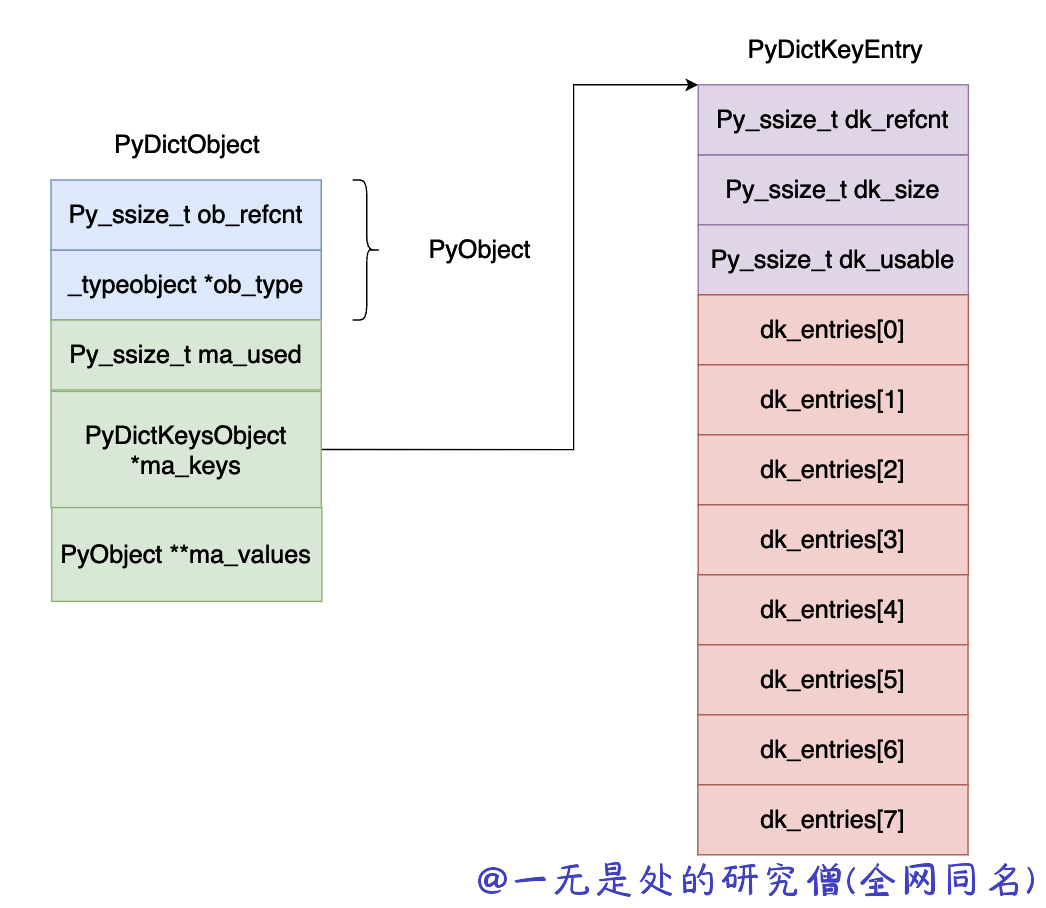
\includegraphics[scale=.25]{images/31-bytes.png}
						\caption{ }
        \label{fig:my_label}
    \end{figure}
    
所有的键值对都存储在 dk\_entries 数组当中,比如对于 "Hello" "World" 这个键值对存储过程如下所示,如果 "Hello" 的哈希值等于 8 ,那么计算出来对象在 dk\_entries 数组当中的下标位 0 。

    \begin{figure}[h]
        \centering
            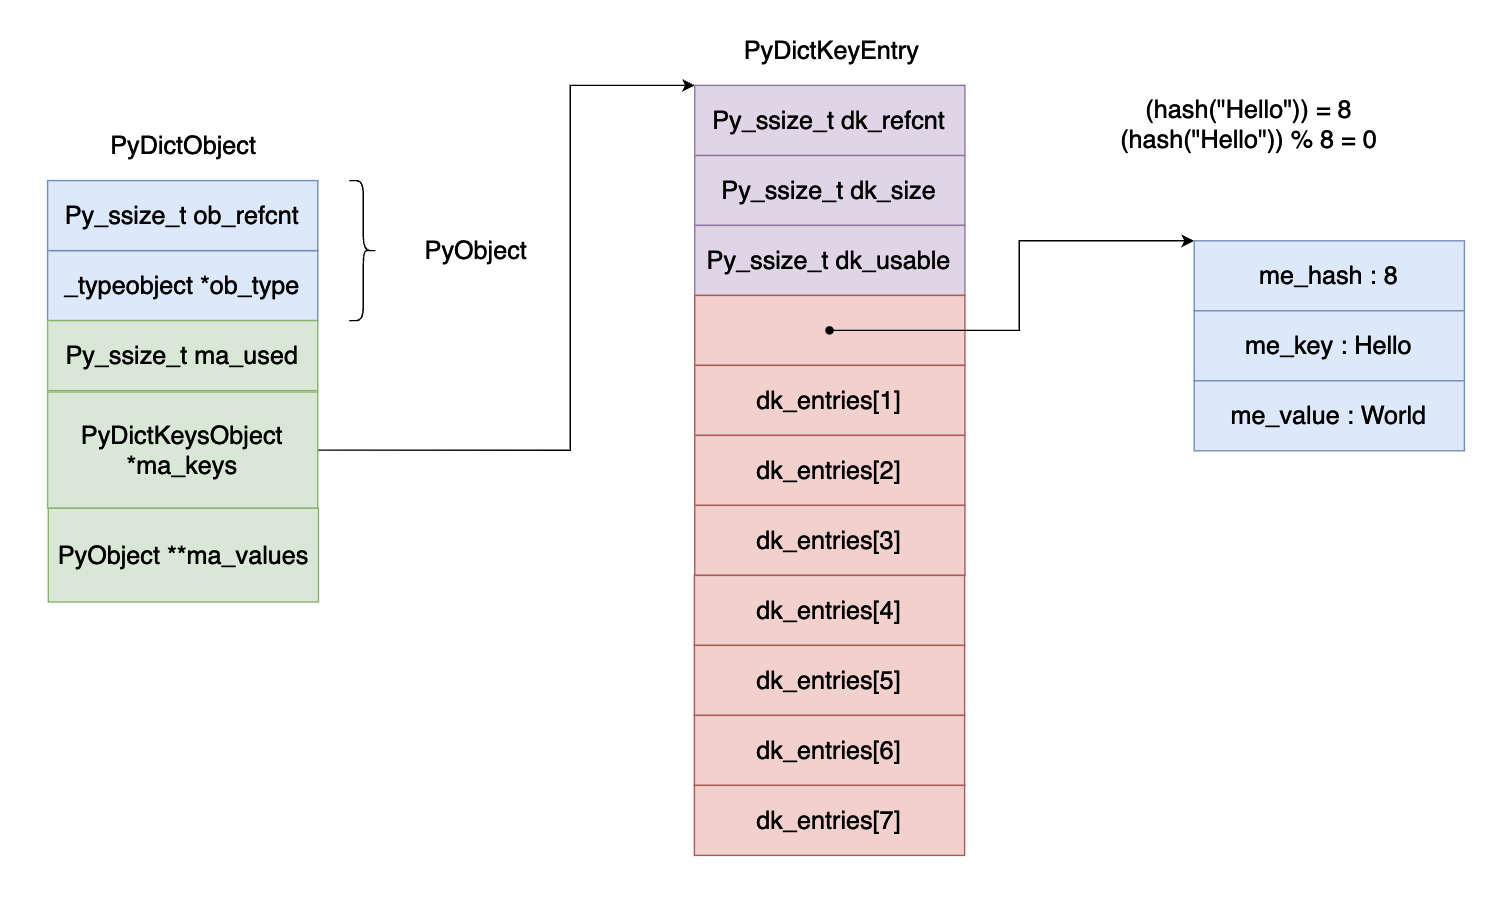
\includegraphics[scale=.25]{images/32-dict.png}
						\caption{ }
        \label{fig:my_label}
    \end{figure}
    
在前面的文章当中我们谈到了,在 cpython 当中 dk\_entries 数组当中的一个对象占用 24 字节的内存空间,在 cpython 当中的负载因子是 $\frac{2}{3}$ 。而一个 entry 的大小是 24 个字节,如果 dk\_entries 的长度是 1024 的话,那么大概有 1024  / 3 * 24 = 8K 的内存空间是浪费的。为了解决这个问题,在新版的 cpython 当中采取了一个策略用于减少内存的使用。具体的设计如下图所示:

    \begin{figure}[h]
        \centering
            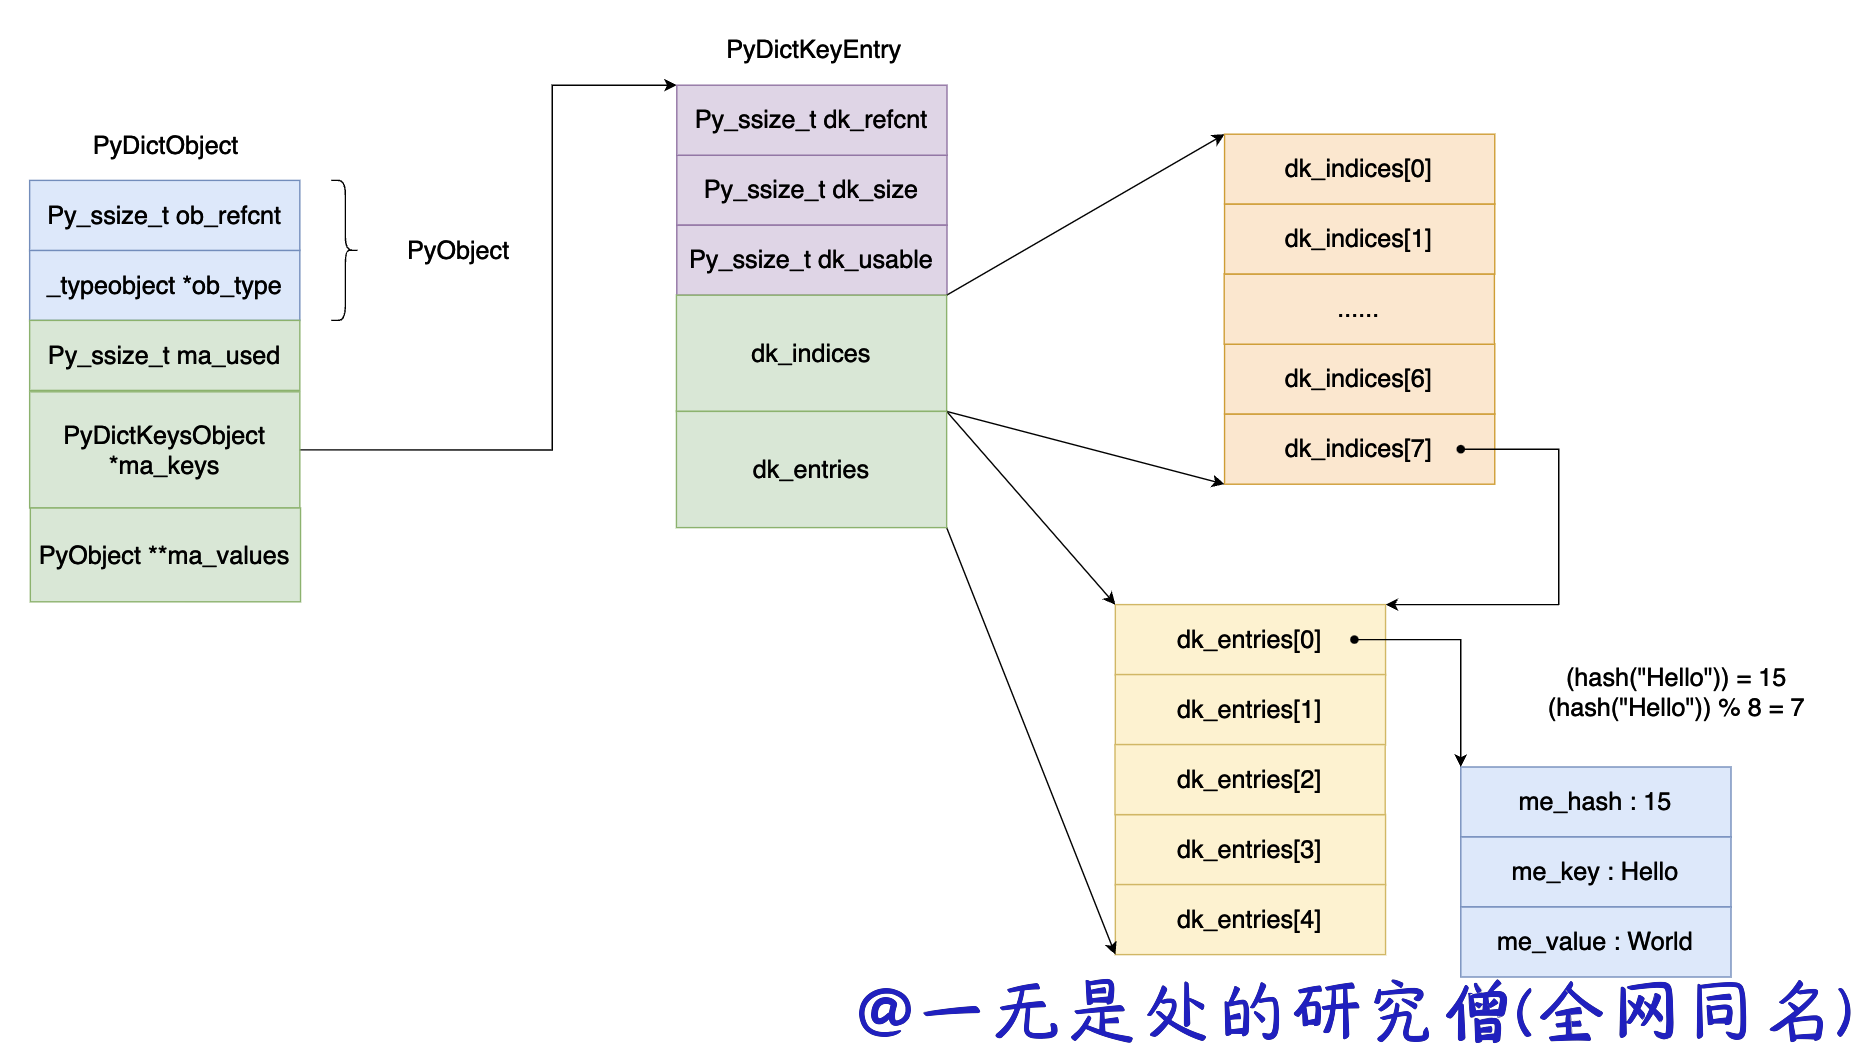
\includegraphics[scale=.2]{images/33-dict.png}
						\caption{ }
        \label{fig:my_label}
    \end{figure}
    
在新的字典当中 cpython 对于 dk\_entries 来说如果正常的哈希表的长度为 8 的话,因为负载因子是 $\frac{2}{3}$ 真正给 dk\_entries 分配的长度是 5 = 8 / 3,那么现在有一个问题就是如何根据不同的哈希值进行对象的存储。dk\_indices 就是这个作用的,他的长度和真正的哈希表的长度是一样的,dk\_indices 是一个整型数组这个数组保存的是要保存对象在 dk\_entries 当中的下标,比如在上面的例子当中 dk\_indices[7] = 0,就表示哈希值求余数之后的值等于 7,0 表示对象在 dk\_entries 当中的下标。
现在我们再插入一个数据 "World" "Hello" 键值对,假设 "World" 的哈希值等于 8,那么对哈希值求余数之后等于 0 ,那么 dk\_indices[0] 就是保存对象在 dk\_entries 数组当中的下标的,图中对应的下标为 1 (因为 dk\_entries 数组当中的每个数据都要使用,因此直接递增即可,下一个对象来的话就保存在 dk\_entries 数组的第 3 个(下标为 2)位置)。

    \begin{figure}[h]
        \centering
            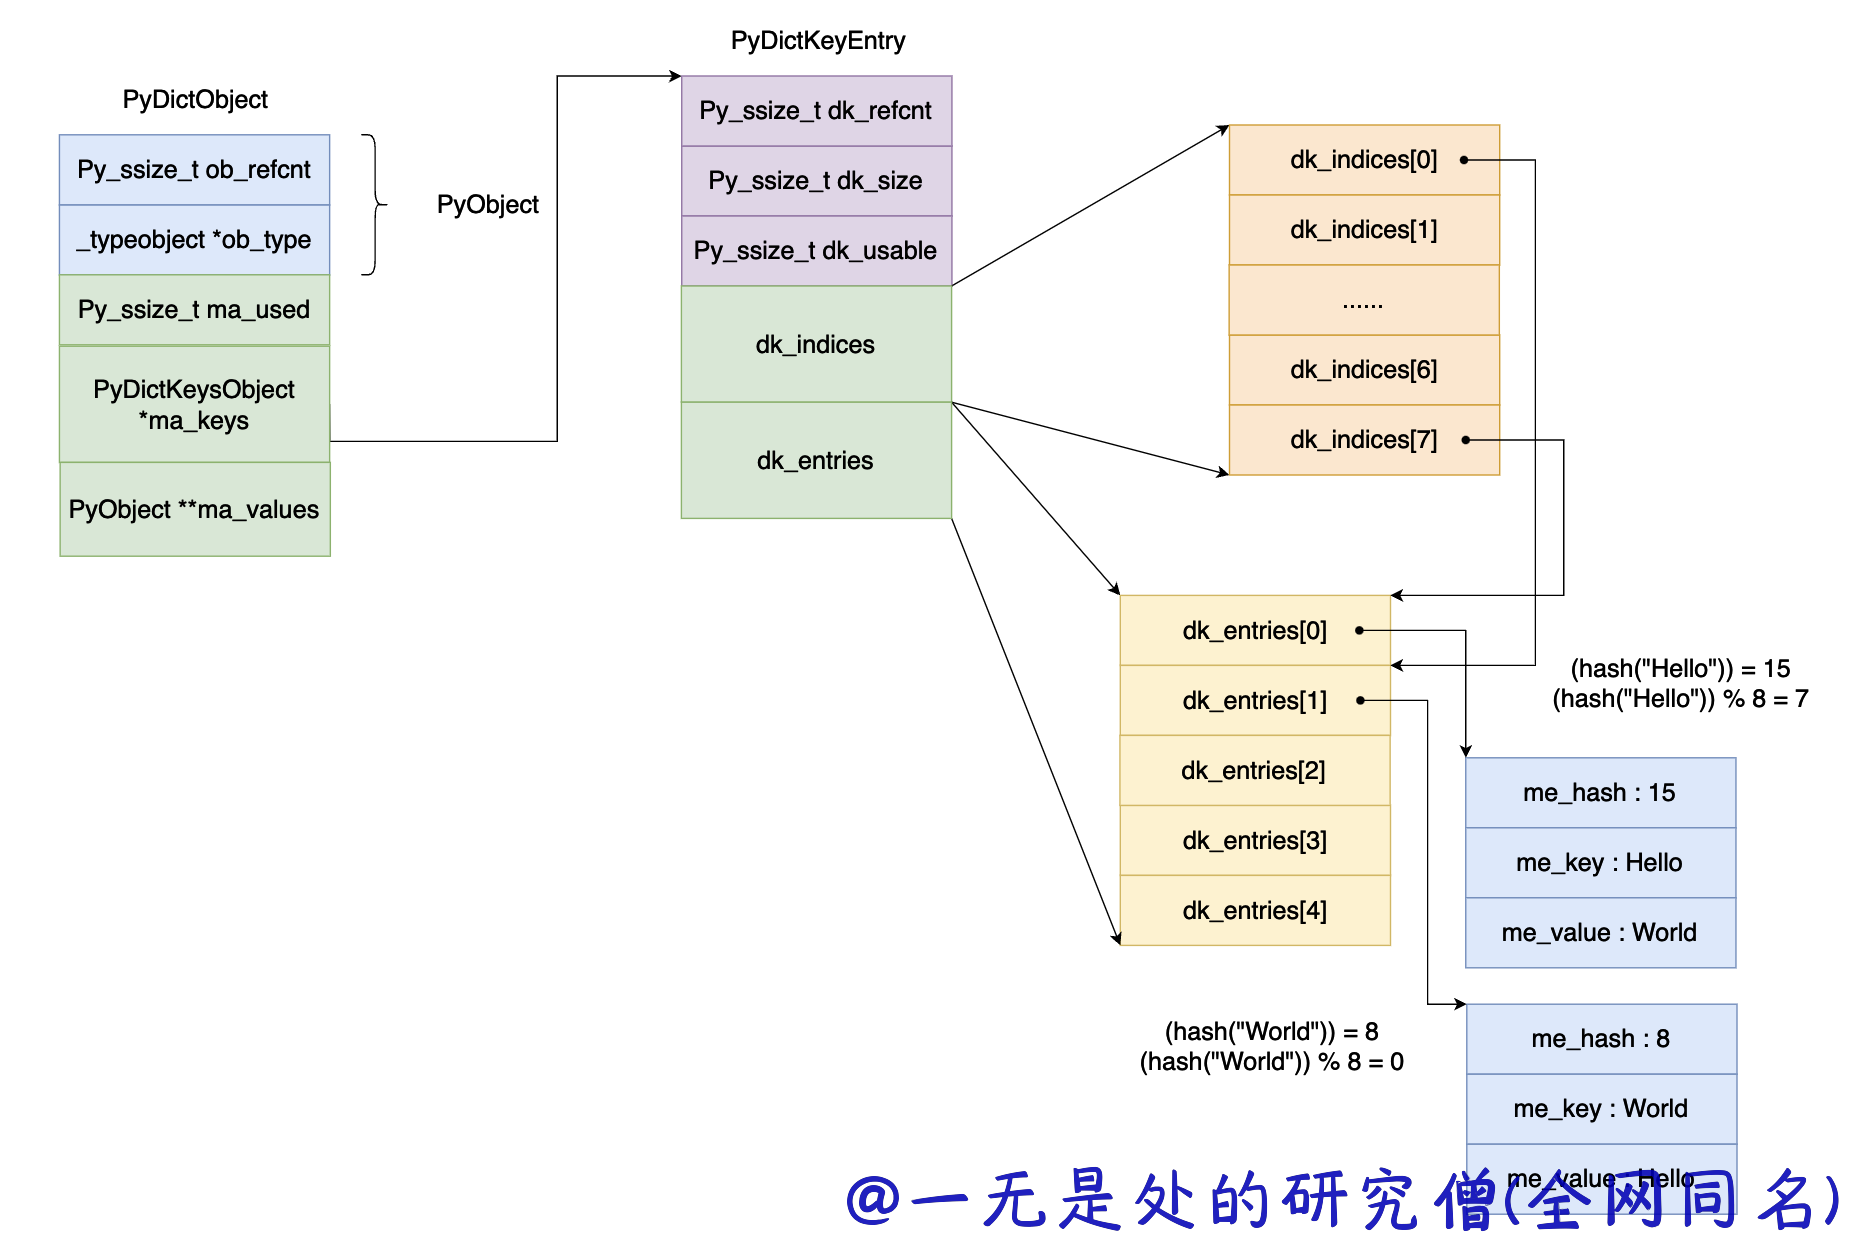
\includegraphics[scale=.2]{images/34-dict.png}
						\caption{ }
        \label{fig:my_label}
    \end{figure}
    
\subsection{内存分析}
首先我们先来分析一下数组 dk\_indices 的数据类型,在 cpython 的内部实现当中并没有一刀切的直接将这个数组当中的数据类型设置成 int 类型。
dk\_indices 数组主要有以下几个类型:
\begin{itemize}
\item 当哈希表长度小于 0xff 时,dk\_indices 的数据类型为 int8\_t ,即一个元素值占一个字节。 
\item 当哈希表长度小于 0xffff 时,dk\_indices 的数据类型为 int16\_t ,即一个元素值占 2 一个字节。 
\item 当哈希表长度小于 0xffffffff 时,dk\_indices 的数据类型为 int32\_t ,即一个元素值占 4 个字节。 
\item 当哈希表长度大于 0xffffffff 时,dk\_indices 的数据类型为 int64\_t ,即一个元素值占 8 个字节。 
\end{itemize}
与这个相关的代码如下所示:
\begin{lstlisting}[style=cpp,caption=, language=C++]

/* lookup indices.  returns DKIX_EMPTY, DKIX_DUMMY, or ix >=0 */
static inline Py_ssize_t
dictkeys_get_index(const PyDictKeysObject *keys, Py_ssize_t i)
{
    Py_ssize_t s = DK_SIZE(keys);
    Py_ssize_t ix;
    if (s <= 0xff) {
        const int8_t *indices = (const int8_t*)(keys->dk_indices);
        ix = indices[i];
    }
    else if (s <= 0xffff) {
        const int16_t *indices = (const int16_t*)(keys->dk_indices);
        ix = indices[i];
    }
#if SIZEOF_VOID_P > 4
    else if (s > 0xffffffff) {
        const int64_t *indices = (const int64_t*)(keys->dk_indices);
        ix = indices[i];
    }
#endif
    else {
        const int32_t *indices = (const int32_t*)(keys->dk_indices);
        ix = indices[i];
    }
    assert(ix >= DKIX_DUMMY);
    return ix;
}
\end{lstlisting}
现在来分析一下相关的内存使用情况:
\begin{table}[]
    \centering
        \begin{tabular}{|c|c|c|c|c|}
        \hline
        \textbf{哈希表长度} & \textbf{能够保存的键值对数目} & \textbf{老版本} & \textbf{新版本} & \textbf{节约内存量(字节)}  \\
        \hline
        256 & 170 & 6144 & 4336 & 1808 \\
        \hline
        65536 & 43690 & 1572864 & 1179632 & 393232 \\
        \hline
        \end{tabular}
    \caption{哈希表内存消耗情况对比}
    \label{tab:my_label}
\end{table}

从上面的表格我们可以看到哈希表的长度越大我们节约的内存就越大,优化的效果就越明显。
\subsection{总结}
在本小节当中主要介绍了在 python3 当中对于字典的优化操作,主要是通过一个内存占用量比较小的数组去保存键值对在真实保存键值对当中的下标实现的,这个方法对于节约内存的效果是非常明显的。

\section{集合(set)的实现原理及源码剖析}
在本小节当中主要给大家介绍在 cpython 虚拟机当中的集合 set 的实现原理以及对应的源代码分析。
\subsection{数据结构介绍}
\begin{lstlisting}[style=cpp,caption=, language=C++]

typedef struct {
    PyObject_HEAD
    Py_ssize_t fill;            /* Number active and dummy entries*/
    Py_ssize_t used;            /* Number active entries */
    /* The table contains mask + 1 slots, and that's a power of 2.
     * We store the mask instead of the size because the mask is more
     * frequently needed.
     */
    Py_ssize_t mask;
    /* The table points to a fixed-size smalltable for small tables
     * or to additional malloc'ed memory for bigger tables.
     * The table pointer is never NULL which saves us from repeated
     * runtime null-tests.
     */
    setentry *table;
    Py_hash_t hash;             /* Only used by frozenset objects */
    Py_ssize_t finger;          /* Search finger for pop() */
    setentry smalltable[PySet_MINSIZE]; // #define PySet_MINSIZE 8
    PyObject *weakreflist;      /* List of weak references */
} PySetObject;
typedef struct {
    PyObject *key;
    Py_hash_t hash;             /* Cached hash code of the key */
} setentry;
static PyObject _dummy_struct;
#define dummy (&_dummy_struct)
\end{lstlisting}
上面的数据结果用图示如下图所示:

    \begin{figure}[h]
        \centering
            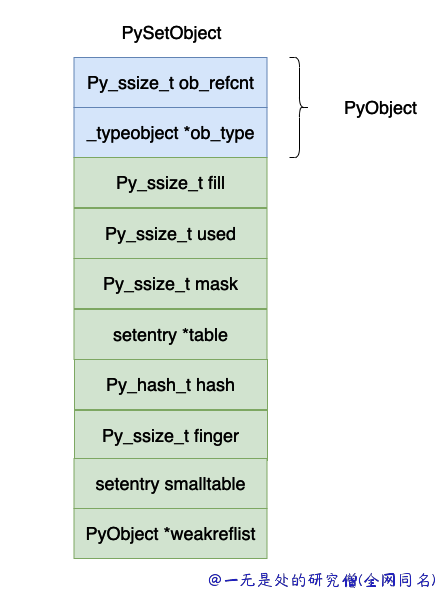
\includegraphics[scale=.5]{images/25-set.png}
            \caption{ }
        \label{fig:my_label}
    \end{figure}
    
上面各个字段的含义如下所示:
\begin{itemize}
\item dummy entries :如果在哈希表当中的数组原来有一个数据,如果我们删除这个 entry 的时候,对应的位置就会被赋值成 dummy,与 dummy 有关的定义在上面的代码当中已经给出,dummy 对象的哈希值等于 -1。 
\item 明白 dummy 的含义之后,fill 和 used 这两个字段的含义就比较容易理解了,used 就是数组当中真实有效的对象的个数,fill 还需要加上 dummy 对象的个数。 
\item mask,数组的长度等于 $2^n$,mask 的值等于 $2^n - 1$ 。 
\item table,实际保存 entry 对象的数组。 
\item hash,这个值对 frozenset 有用,保存计算出来的哈希值。如果你的数组很大的话,计算哈希值其实也是一个比较大的开销,因此可以将计算出来的哈希值保存下来,以便下一次求的时候可以将哈希值直接返回,这也印证了在 python 当中为什么只有 immutable 对象才能够放入到集合和字典当中,因为哈希值计算一次保存下来了,如果再加入对象对象的哈希值也会变化,这样做就会发生错误了。 
\item finger,主要是用于记录下一个开始寻找被删除对象的下标。 
\item smalltable,默认的小数组,cpython 设置的一半的集合对象不会超过这个大小(8),因此在申请一个集合对象的时候直接就申请了这个小数组的内存大小。 
\item weakrelist,这个字段主要和垃圾回收有关,这里暂时不进行详细说明。 
\end{itemize}
\subsection{创建集合对象}
首先先了解一下创建一个集合对象的过程,和前面其他的对象是一样的,首先先申请内存空间,然后进行相关的初始化操作。
这个函数有两个参数,使用第一个参数申请内存空间,然后后面一个参数如果不为 NULL 而且是一个可迭代对象的话,就将这里面的对象加入到集合当中。
\begin{lstlisting}[style=cpp,caption=, language=C++]

static PyObject *
make_new_set(PyTypeObject *type, PyObject *iterable)
{
    PySetObject *so = NULL;
    /* create PySetObject structure */
    so = (PySetObject *)type->tp_alloc(type, 0);
    if (so == NULL)
        return NULL;
    // 集合当中目前没有任何对象,因此 fill 和 used 都是 0
    so->fill = 0;
    so->used = 0;
    // 初始化哈希表当中的数组长度为 PySet_MINSIZE 因此 mask = PySet_MINSIZE - 1
    so->mask = PySet_MINSIZE - 1;
    // 让 table 指向存储 entry 的数组
    so->table = so->smalltable;
    // 将哈希值设置成 -1 表示还没有进行计算
    so->hash = -1;
    so->finger = 0;
    so->weakreflist = NULL;
    // 如果 iterable 不等于 NULL 则需要将它指向的对象当中所有的元素加入到集合当中
    if (iterable != NULL) {
        // 调用函数 set_update_internal 将对象 iterable 当中的元素加入到集合当中
        if (set_update_internal(so, iterable)) {
            Py_DECREF(so);
            return NULL;
        }
    }
    return (PyObject *)so;
}
\end{lstlisting}
\subsection{往集合当中加入数据}
首先我们先大致理清楚往集合当中插入数据的流程:
\begin{itemize}
\item 首先根据对象的哈希值,计算需要将对象放在哪个位置,也就是对应数组的下标。 
\item 查看对应下标的位置是否存在对象,如果不存在对象则将数据保存在对应下标的位置。 
\item 如果对应的位置存在对象,则查看是否和当前要插入的对象相等,则返回。 
\item 如果不相等,则使用类似于线性探测的方式去寻找下一个要插入的位置(具体的实现可以查看相关代码,具体的操作为线性探测法 + 开放地址法)。 
\end{itemize}
\begin{lstlisting}[style=cpp,caption=, language=C++]

static PyObject *
set_add(PySetObject *so, PyObject *key)
{
    if (set_add_key(so, key))
        return NULL;
    Py_RETURN_NONE;
}
static int
set_add_key(PySetObject *so, PyObject *key)
{
    setentry entry;
    Py_hash_t hash;
    // 这里就查看一下是否是字符串,如果是字符串直接拿到哈希值
    if (!PyUnicode_CheckExact(key) ||
        (hash = ((PyASCIIObject *) key)->hash) == -1) {
      	// 如果不是字符串则需要调用对象自己的哈希函数求得对应的哈希值
        hash = PyObject_Hash(key);
        if (hash == -1)
            return -1;
    }
    // 创建一个 entry 对象将这个对象加入到哈希表当中
    entry.key = key;
    entry.hash = hash;
    return set_add_entry(so, &entry);
}
static int
set_add_entry(PySetObject *so, setentry *entry)
{
    Py_ssize_t n_used;
    PyObject *key = entry->key;
    Py_hash_t hash = entry->hash;
    assert(so->fill <= so->mask);  /* at least one empty slot */
    n_used = so->used;
    Py_INCREF(key);
    // 调用函数 set_insert_key 将对象插入到数组当中
    if (set_insert_key(so, key, hash)) {
        Py_DECREF(key);
        return -1;
    }
    // 这里就是哈希表的核心的扩容机制
    if (!(so->used > n_used && so->fill*3 >= (so->mask+1)*2))
        return 0;
    // 这是扩容大小的逻辑
    return set_table_resize(so, so->used>50000 ? so->used*2 : so->used*4);
}
static int
set_insert_key(PySetObject *so, PyObject *key, Py_hash_t hash)
{
    setentry *entry;
    // set_lookkey 这个函数便是插入的核心的逻辑的实现对应的实现函数在下方
    entry = set_lookkey(so, key, hash);
    if (entry == NULL)
        return -1;
    if (entry->key == NULL) {
        /* UNUSED */
        entry->key = key;
        entry->hash = hash;
        so->fill++;
        so->used++;
    } else if (entry->key == dummy) {
        /* DUMMY */
        entry->key = key;
        entry->hash = hash;
        so->used++;
    } else {
        /* ACTIVE */
        Py_DECREF(key);
    }
    return 0;
}
// 下面的代码就是在执行我们在前面所谈到的逻辑,直到找到相同的 key 或者空位置才退出 while 循环
static setentry *
set_lookkey(PySetObject *so, PyObject *key, Py_hash_t hash)
{
    setentry *table = so->table;
    setentry *freeslot = NULL;
    setentry *entry;
    size_t perturb = hash;
    size_t mask = so->mask;
    size_t i = (size_t)hash & mask; /* Unsigned for defined overflow behavior */
    size_t j;
    int cmp;
    entry = &table[i];
    if (entry->key == NULL)
        return entry;
    while (1) {
        if (entry->hash == hash) {
            PyObject *startkey = entry->key;
            /* startkey cannot be a dummy because the dummy hash field is -1 */
            assert(startkey != dummy);
            if (startkey == key)
                return entry;
            if (PyUnicode_CheckExact(startkey)
                && PyUnicode_CheckExact(key)
                && unicode_eq(startkey, key))
                return entry;
            Py_INCREF(startkey);
            // returning -1 for error, 0 for false, 1 for true
            cmp = PyObject_RichCompareBool(startkey, key, Py_EQ);
            Py_DECREF(startkey);
            if (cmp < 0)                                          /* unlikely */
                return NULL;
            if (table != so->table || entry->key != startkey)     /* unlikely */
                return set_lookkey(so, key, hash);
            if (cmp > 0)                                          /* likely */
                return entry;
            mask = so->mask;                 /* help avoid a register spill */
        }
        if (entry->hash == -1 && freeslot == NULL)
            freeslot = entry;
        if (i + LINEAR_PROBES <= mask) {
            for (j = 0 ; j < LINEAR_PROBES ; j++) {
                entry++;
                if (entry->key == NULL)
                    goto found_null;
                if (entry->hash == hash) {
                    PyObject *startkey = entry->key;
                    assert(startkey != dummy);
                    if (startkey == key)
                        return entry;
                    if (PyUnicode_CheckExact(startkey)
                        && PyUnicode_CheckExact(key)
                        && unicode_eq(startkey, key))
                        return entry;
                    Py_INCREF(startkey);
                    // returning -1 for error, 0 for false, 1 for true
                    cmp = PyObject_RichCompareBool(startkey, key, Py_EQ);
                    Py_DECREF(startkey);
                    if (cmp < 0)
                        return NULL;
                    if (table != so->table || entry->key != startkey)
                        return set_lookkey(so, key, hash);
                    if (cmp > 0)
                        return entry;
                    mask = so->mask;
                }
                if (entry->hash == -1 && freeslot == NULL)
                    freeslot = entry;
            }
        }
        perturb >>= PERTURB_SHIFT; // #define PERTURB_SHIFT 5
        i = (i * 5 + 1 + perturb) & mask;
        entry = &table[i];
        if (entry->key == NULL)
            goto found_null;
    }
  found_null:
    return freeslot == NULL ? entry : freeslot;
}
\end{lstlisting}
\subsection{哈希表数组扩容}
在 cpython 当中对于给哈希表数组扩容的操作,很多情况下都是用下面这行代码,从下面的代码来看对应扩容后数组的大小并不简单,当你的哈希表当中的元素个数大于 50000 时,新数组的大小是原数组的两倍,而如果你哈希表当中的元素个数小于等于 50000,那么久扩大为原来长度的四倍,这个主要是怕后面如果继续扩大四倍的话,可能会浪费很多内存空间。
\begin{lstlisting}[style=cpp,caption=, language=C++]

set_table_resize(so, so->used>50000 ? so->used*2 : so->used*4);
\end{lstlisting}
首先需要了解一下扩容机制,当哈希表需要扩容的时候,主要有以下两个步骤:
\begin{itemize}
\item 创建新的数组,用于存储哈希表的键。 
\item 遍历原来的哈希表,将原来哈希表当中的数据加入到新的申请的数组当中。 
\end{itemize}
这里需要注意的是因为数组的长度发生了变化,但是 key 的哈希值却没有发生变化,因此在新的数组当中数据对应的下标位置也会发生变化,因此需重新将所有的对象重新进行一次插入操作,下面的整个操作相对来说比较简单,这里不再进行说明了。
\begin{lstlisting}[style=cpp,caption=, language=C++]

static int
set_table_resize(PySetObject *so, Py_ssize_t minused)
{
    Py_ssize_t newsize;
    setentry *oldtable, *newtable, *entry;
    Py_ssize_t oldfill = so->fill;
    Py_ssize_t oldused = so->used;
    int is_oldtable_malloced;
    setentry small_copy[PySet_MINSIZE];
    assert(minused >= 0);
    /* Find the smallest table size > minused. */
    /* XXX speed-up with intrinsics */
    for (newsize = PySet_MINSIZE;
         newsize <= minused && newsize > 0;
         newsize <<= 1)
        ;
    if (newsize <= 0) {
        PyErr_NoMemory();
        return -1;
    }
    /* Get space for a new table. */
    oldtable = so->table;
    assert(oldtable != NULL);
    is_oldtable_malloced = oldtable != so->smalltable;
    if (newsize == PySet_MINSIZE) {
        /* A large table is shrinking, or we can't get any smaller. */
        newtable = so->smalltable;
        if (newtable == oldtable) {
            if (so->fill == so->used) {
                /* No dummies, so no point doing anything. */
                return 0;
            }
            /* We're not going to resize it, but rebuild the
               table anyway to purge old dummy entries.
               Subtle:  This is *necessary* if fill==size,
               as set_lookkey needs at least one virgin slot to
               terminate failing searches.  If fill < size, it's
               merely desirable, as dummies slow searches. */
            assert(so->fill > so->used);
            memcpy(small_copy, oldtable, sizeof(small_copy));
            oldtable = small_copy;
        }
    }
    else {
        newtable = PyMem_NEW(setentry, newsize);
        if (newtable == NULL) {
            PyErr_NoMemory();
            return -1;
        }
    }
    /* Make the set empty, using the new table. */
    assert(newtable != oldtable);
    memset(newtable, 0, sizeof(setentry) * newsize);
    so->fill = 0;
    so->used = 0;
    so->mask = newsize - 1;
    so->table = newtable;
    /* Copy the data over; this is refcount-neutral for active entries;
       dummy entries aren't copied over, of course */
    if (oldfill == oldused) {
        for (entry = oldtable; oldused > 0; entry++) {
            if (entry->key != NULL) {
                oldused--;
                set_insert_clean(so, entry->key, entry->hash);
            }
        }
    } else {
        for (entry = oldtable; oldused > 0; entry++) {
            if (entry->key != NULL && entry->key != dummy) {
                oldused--;
                set_insert_clean(so, entry->key, entry->hash);
            }
        }
    }
    if (is_oldtable_malloced)
        PyMem_DEL(oldtable);
    return 0;
}
static void
set_insert_clean(PySetObject *so, PyObject *key, Py_hash_t hash)
{
    setentry *table = so->table;
    setentry *entry;
    size_t perturb = hash;
    size_t mask = (size_t)so->mask;
    size_t i = (size_t)hash & mask;
    size_t j;
    // #define LINEAR_PROBES 9
    while (1) {
        entry = &table[i];
        if (entry->key == NULL)
            goto found_null;
        if (i + LINEAR_PROBES <= mask) {
            for (j = 0; j < LINEAR_PROBES; j++) {
                entry++;
                if (entry->key == NULL)
                    goto found_null;
            }
        }
        perturb >>= PERTURB_SHIFT;
        i = (i * 5 + 1 + perturb) & mask;
    }
  found_null:
    entry->key = key;
    entry->hash = hash;
    so->fill++;
    so->used++;
}
\end{lstlisting}
\subsection{从集合当中删除元素 pop}
从集合当中删除元素的代码如下所示:
\begin{lstlisting}[style=cpp,caption=, language=C++]

static PyObject *
set_pop(PySetObject *so)
{
    /* Make sure the search finger is in bounds */
    Py_ssize_t i = so->finger & so->mask;
    setentry *entry;
    PyObject *key;
    assert (PyAnySet_Check(so));
    if (so->used == 0) {
        PyErr_SetString(PyExc_KeyError, "pop from an empty set");
        return NULL;
    }
    while ((entry = &so->table[i])->key == NULL || entry->key==dummy) {
        i++;
        if (i > so->mask)
            i = 0;
    }
    key = entry->key;
    entry->key = dummy;
    entry->hash = -1;
    so->used--;
    so->finger = i + 1;         /* next place to start */
    return key;
}
\end{lstlisting}
上面的代码相对来说也比较清晰,从 finger 开始寻找存在的元素,并且删除他。我们在前面提到过,当一个元素被删除之后他会被赋值成 dummy 而且哈希值为 -1 。
\subsection{总结}
在本小节当中主要给大家简要介绍了一下在 cpython 当中的集合对象是如何实现的,主要是介绍了一些核心的数据结构和 cpython 当中具体的哈希表的实现原理,在 cpython 内部是使用线性探测法和开放地址法两种方法去解决哈希冲突的,同时 cpython 哈希表的扩容方式比价有意思,在哈希表当中的元素个数小于 50000 时,扩容的时候,扩容大小为原来的四倍,当大于 50000 时,扩容的大小为原来的两倍,这个主要是因为怕后面如果扩容太大没有使用非常浪费内存空间。

\chapter{python 虚拟机中基本数据类型}
\section{复数(complex)的实现原理及源码剖析}
在本小节当中主要给大家介绍在 cpython 虚拟机当中是如何实现 复数 complex 这个数据类型的,这个数据类型在 cpython 当中一应该是一个算比较简单的数据类型了,非常容易理解。
\subsection{复数数据结构}
在 cpython 当中对于复数的数据结构实现如下所示:
\begin{lstlisting}[style=cpp,caption=, language=C++]

typedef struct {
    double real;
    double imag;
} Py_complex;
#define PyObject_HEAD                   PyObject ob_base;
typedef struct {
    PyObject_HEAD
    Py_complex cval;
} PyComplexObject;
typedef struct _object {
    _PyObject_HEAD_EXTRA
    Py_ssize_t ob_refcnt;
    struct _typeobject *ob_type;
} PyObject;
\end{lstlisting}
上面的数据结构图示如下:

    \begin{figure}[h]
        \centering
            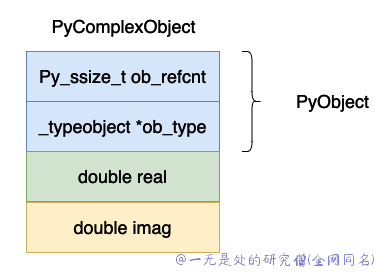
\includegraphics[scale=.5]{images/23-int.png}
            \caption{ }
        \label{fig:my_label}
    \end{figure}
    
复数的数据在整个 cpython 虚拟机当中来说应该算是比较简单的了,除了一个 PyObject 头部之外就是实部和虚部了。
\begin{itemize}
\item ob\_refcnt,表示对象的引用记数的个数,这个对于垃圾回收很有用处,后面我们分析虚拟机中垃圾回收部分在深入分析。 
\item ob\_type,表示这个对象的数据类型是什么,在 python 当中有时候需要对数据的数据类型进行判断比如 isinstance, type 这两个关键字就会使用到这个字段。 
\item real,表示复数的实部。 
\item imag,表示复数的虚部。 
\end{itemize}
\subsection{复数的操作}
\subsubsection{复数加法}
下面是 cpython 当中对于复数加法的实现,为了简洁删除了部分无用代码。
\begin{lstlisting}[style=cpp,caption=, language=C++]

static PyObject *
complex_add(PyObject *v, PyObject *w)
{
    Py_complex result;
    Py_complex a, b;
    TO_COMPLEX(v, a); // TO_COMPLEX 这个宏的作用就是将一个 PyComplexObject 中的 Py_complex 对象存储到 a 当中
    TO_COMPLEX(w, b);
    result = _Py_c_sum(a, b); // 这个函数的具体实现在下方
    return PyComplex_FromCComplex(result); // 这个函数的具体实现在下方
}
// 真正实现复数加法的函数
Py_complex
_Py_c_sum(Py_complex a, Py_complex b)
{
    Py_complex r;
    r.real = a.real + b.real;
    r.imag = a.imag + b.imag;
    return r;
}
PyObject *
PyComplex_FromCComplex(Py_complex cval)
{
    PyComplexObject *op;
    /* Inline PyObject_New */
    // 申请内存空间
    op = (PyComplexObject *) PyObject_MALLOC(sizeof(PyComplexObject));
    if (op == NULL)
        return PyErr_NoMemory();
    // 将这个对象的引用计数设置成 1
    (void)PyObject_INIT(op, &PyComplex_Type);
    // 将复数结构体保存下来
    op->cval = cval;
    return (PyObject *) op;
}
\end{lstlisting}
上面代码的整体过程比较简单:
\begin{itemize}
\item 首先先从 PyComplexObject 提取真正的复数部分。 
\item 将提取到的两个复数进行相加操作。 
\item 根据得到的结果在创建一个 PyComplexObject 对象,并且将这个对象返回。 
\end{itemize}
\subsubsection{复数取反}
复数取反操作就是将实部和虚部取相反数就可以了,这个操作也比较简单。
\begin{lstlisting}[style=cpp,caption=, language=C++]

static PyObject *
complex_neg(PyComplexObject *v)
{
    Py_complex neg;
    neg.real = -v->cval.real;
    neg.imag = -v->cval.imag;
    return PyComplex_FromCComplex(neg);
}
PyObject *
PyComplex_FromCComplex(Py_complex cval)
{
    PyComplexObject *op;
    /* Inline PyObject_New */
    op = (PyComplexObject *) PyObject_MALLOC(sizeof(PyComplexObject));
    if (op == NULL)
        return PyErr_NoMemory();
    (void)PyObject_INIT(op, &PyComplex_Type);
    op->cval = cval;
    return (PyObject *) op;
}
\end{lstlisting}
\subsubsection{Repr 函数}
我们现在来介绍一下一个有趣的方法,就是复数类型的 repr 函数,这个和类的 \_\_repr\_\_ 函数是作用是一样的我们看一下复数的输出是什么:

\begin{lstlisting}[style=py,caption=, language=Python]

>>> data = complex(0, 1)
>>> data
1j
>>> data = complex(1, 1)
>>> data
(1+1j)
>>> print(data)
(1+1j)
\end{lstlisting}
复数的 repr 对应的 C 函数如下所示:
\begin{lstlisting}[style=cpp,caption=, language=C++]

static PyObject *
complex_repr(PyComplexObject *v)
{
    int precision = 0;
    char format_code = 'r';
    PyObject *result = NULL;
    /* If these are non-NULL, they'll need to be freed. */
    char *pre = NULL;
    char *im = NULL;
    /* These do not need to be freed. re is either an alias
       for pre or a pointer to a constant.  lead and tail
       are pointers to constants. */
    char *re = NULL;
    char *lead = "";
    char *tail = "";
    // 对应实部等于 0 虚部大于 0 的情况
    if (v->cval.real == 0. && copysign(1.0, v->cval.real)==1.0) {
        /* Real part is +0: just output the imaginary part and do not
           include parens. */
        re = "";
        im = PyOS_double_to_string(v->cval.imag, format_code,
                                   precision, 0, NULL);
        if (!im) {
            PyErr_NoMemory();
            goto done;
        }
    } else {
        /* Format imaginary part with sign, real part without. Include
           parens in the result. */
        // 将实部浮点数变成字符串
        pre = PyOS_double_to_string(v->cval.real, format_code,
                                    precision, 0, NULL);
        if (!pre) {
            PyErr_NoMemory();
            goto done;
        }
        re = pre;
        // 将虚部浮点数变成字符串
        im = PyOS_double_to_string(v->cval.imag, format_code,
                                   precision, Py_DTSF_SIGN, NULL);
        if (!im) {
            PyErr_NoMemory();
            goto done;
        }
        // 用什么括号包围起来
        lead = "(";
        tail = ")";
    }
    result = PyUnicode_FromFormat("%s%s%sj%s", lead, re, im, tail);
  done:
    PyMem_Free(im);
    PyMem_Free(pre);
    return result;
}
\end{lstlisting}
我们现在修改源程序将上面的 () 两个括号变成 [],编译之后执行的结果如下所示:

    \begin{figure}[h]
        \centering
            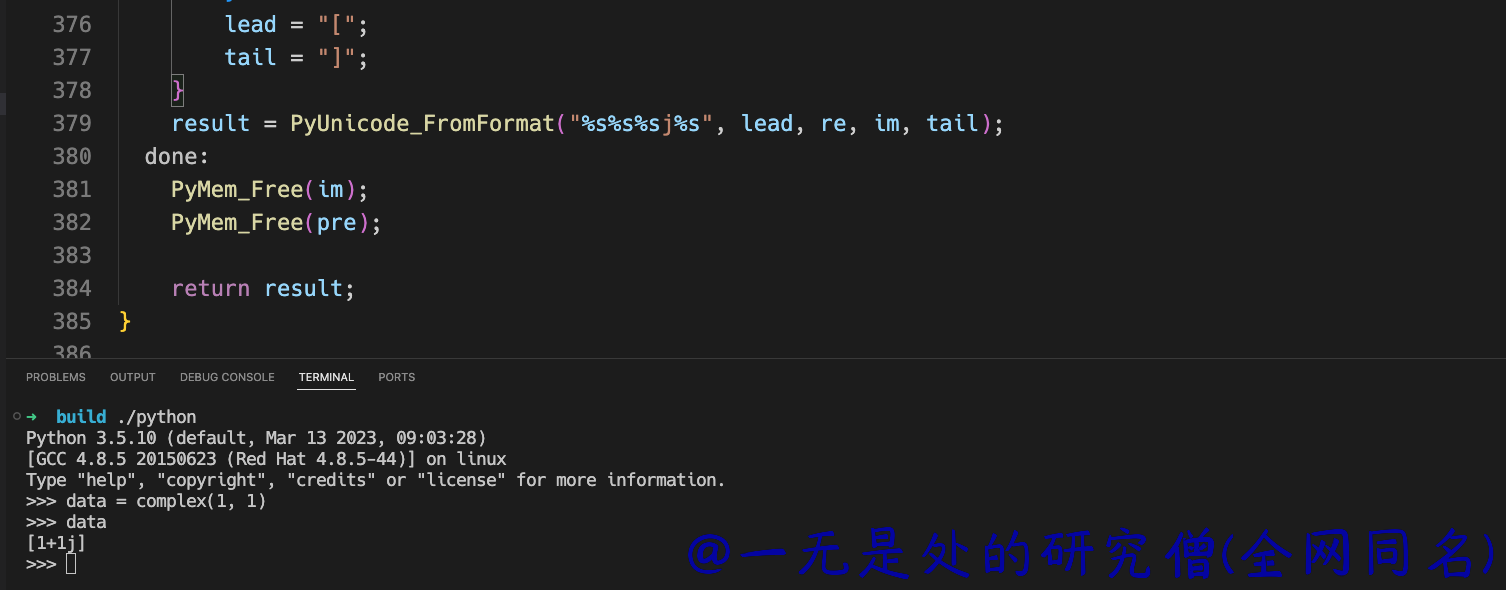
\includegraphics[scale=.3]{images/24-int.png}
            \caption{ }
        \label{fig:my_label}
    \end{figure}
    
可以看到括号变成了 [] 。
\subsection{总结}
在本小节当中主要给大家介绍了在 cpython 虚拟机当中对于复数这一类型的数据结构以及他的具体实现。总体来说这个数据结构比较简单,操作也相对容易,比较容易理解,最后简单介绍了一下复数类型的 repr 实现,其实这个函数和 python 的类型系统有关,目前我们还没有仔细去讨论这一点,在后续的文章当中我们将深入的去学习这个知识点,现在我们就先了解其中部分函数即可。
\section{浮点数(float)的实现原理及源码剖析}
在本小节当中主要分析在 cpython 虚拟机当中 float 类型的实现原理以及与他相关的一些源代码。
\subsection{Float 数据结构}
在 cpython 虚拟机当中浮点数类型的数据结构定义如下所示:
\begin{lstlisting}[style=cpp,caption=, language=C++]

typedef struct {
    PyObject_HEAD
    double ob_fval;
} PyFloatObject;
\end{lstlisting}
上面的数据结构定义图示如下:

    \begin{figure}[h]
        \centering
            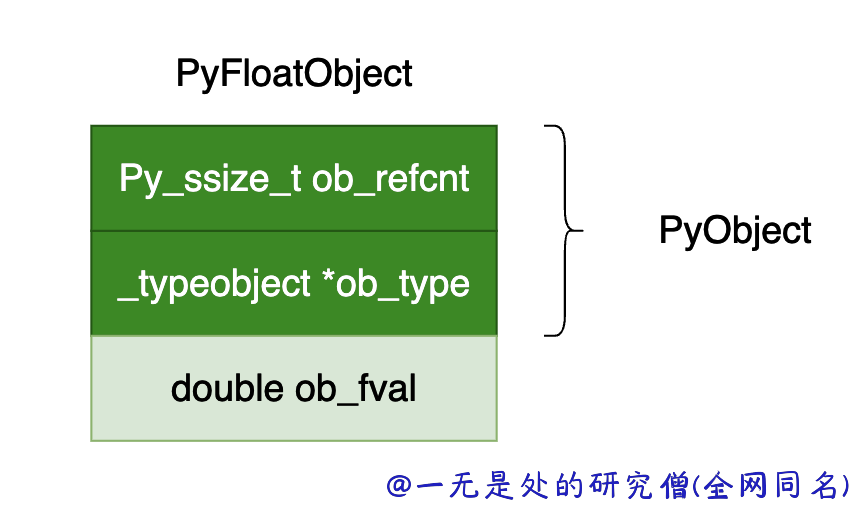
\includegraphics[scale=.4]{images/12-tuple.png}
            \caption{ }
        \label{fig:my_label}
    \end{figure}
    
\begin{itemize}
\item 在上面的数据结构当中最重要的一个字段就是 ob\_fval,这个就是真实存储浮点数的地方。 
\item ob\_refcnt 就是对象的引用计数。 
\item ob\_type 就是对象的类型。 
\end{itemize}
\subsection{浮点数的相关方法}
\subsubsection{创建 float 对象}
和我们在前面所讨论到的元组和列表对象一样,在 cpython 内部实现 float 类型的时候也会给 float 对象做一层中间层以加快浮点数的内存分配,具体的相关代码如下所示:
\begin{lstlisting}[style=cpp,caption=, language=C++]

#define PyFloat_MAXFREELIST    100
static int numfree = 0;
static PyFloatObject *free_list = NULL;
\end{lstlisting}
在 cpython 内部做多会缓存 100 个 float 对象的内存空间,如果超过 100 就会直接释放内存了,这里需要注意一点的是只用一个指针就可以将所有的 float 对象缓存起来,这一点是如何实现的。
这是使用在对象 PyFloatObject 当中的 struct \_typeobject *ob\_type; 这个字段实现的,用这个字段指向下一个 float 对象的内存空间,因为在 free\_list 当中的数据并没有使用,因此可以利用这个特点节省一些内存空间。下面则是创建 float 对象的具体过程:
\begin{lstlisting}[style=cpp,caption=, language=C++]

PyObject *
PyFloat_FromDouble(double fval)
{
    // 首先查看 free_list 当中是否有空闲的 float 对象
    PyFloatObject *op = free_list;
    if (op != NULL) {
        // 如果有 那么就将让 free_list 指向 free_list 当中的下一个 float 对象 并且将对应的个数减 1
        free_list = (PyFloatObject *) Py_TYPE(op);
        numfree--;
    } else {
      	// 否则的话就需要申请内存空间
        op = (PyFloatObject*) PyObject_MALLOC(sizeof(PyFloatObject));
        if (!op)
            return PyErr_NoMemory();
    }
    /* Inline PyObject_New */
    (void)PyObject_INIT(op, &PyFloat_Type); // PyObject_INIT 这个宏的主要作用是将对象的引用计数设置成 1
    op->ob_fval = fval;
    return (PyObject *) op;
}
\end{lstlisting}
\subsubsection{加法}
下面是在 cpython 当中浮点数的加法具体实现,整个过程比较简单就是得到新的值,并且创建一个新的 PyFloatObject 对象,并且将这个对象返回。
\begin{lstlisting}[style=cpp,caption=, language=C++]

static PyObject *
float_add(PyObject *v, PyObject *w)
{
    double a,b;
    CONVERT_TO_DOUBLE(v, a); // CONVERT_TO_DOUBLE 这个宏的主要作用就是将对象的 ob_fval 这个字段的值保存到 a 当中
    CONVERT_TO_DOUBLE(w, b); // 这个就是将 w 当中的 ob_fval 字段的值保存到 b 当中
    a = a + b;
    return PyFloat_FromDouble(a); // 创建一个新的 float 对象 并且将这个对象返回
}
\end{lstlisting}
\subsubsection{减法}
同理减法也是一样的。
\begin{lstlisting}[style=cpp,caption=, language=C++]

static PyObject *
float_sub(PyObject *v, PyObject *w)
{
    double a,b;
    CONVERT_TO_DOUBLE(v, a);
    CONVERT_TO_DOUBLE(w, b);
    a = a _mmb; 
    return PyFloat_FromDouble(a);
}
\end{lstlisting}
\subsubsection{乘法}
\begin{lstlisting}[style=cpp,caption=, language=C++]
static PyObject *
float_mul(PyObject *v, PyObject *w)
{
    double a,b;
    CONVERT_TO_DOUBLE(v, a);
    CONVERT_TO_DOUBLE(w, b);
    PyFPE_START_PROTECT("multiply", return 0)
    a = a * b;
    PyFPE_END_PROTECT(a)
    return PyFloat_FromDouble(a);
}
\end{lstlisting}
\subsubsection{除法}
\begin{lstlisting}[style=cpp,caption=, language=C++]

static PyObject *
float_div(PyObject *v, PyObject *w)
{
    double a,b;
    CONVERT_TO_DOUBLE(v, a);
    CONVERT_TO_DOUBLE(w, b);
    if (b == 0.0) {
        PyErr_SetString(PyExc_ZeroDivisionError,
                        "float division by zero");
        return NULL;
    }
    a = a / b;
    return PyFloat_FromDouble(a);
}
\end{lstlisting}
\subsubsection{取反}
这里加入了一行输出语句,这个是为了后面方便我们进行测试的。
\begin{lstlisting}[style=cpp,caption=, language=C++]

static PyObject *
float_neg(PyFloatObject *v)
{
    printf("%.2lf 正在进行取反运算\n", v->ob_fval);
    return PyFloat_FromDouble(-v->ob_fval);
}
\end{lstlisting}
\subsubsection{求绝对值}
\begin{lstlisting}[style=cpp,caption=, language=C++]

static PyObject *
float_abs(PyFloatObject *v)
{
    printf("%.2lf 正在进行取 abs 运算\n", v->ob_fval);
    return PyFloat_FromDouble(fabs(v->ob_fval));
}
\end{lstlisting}
\subsubsection{求 bool 值}
\begin{lstlisting}[style=cpp,caption=, language=C++]

static int
float_bool(PyFloatObject *v)
{
    printf("%.2lf 正在进行取 bool 运算\n", v->ob_fval);
    return v->ob_fval != 0.0;
}
\end{lstlisting}
下图是我们对于 cpython 对程序的修改!

    \begin{figure}[h]
        \centering
            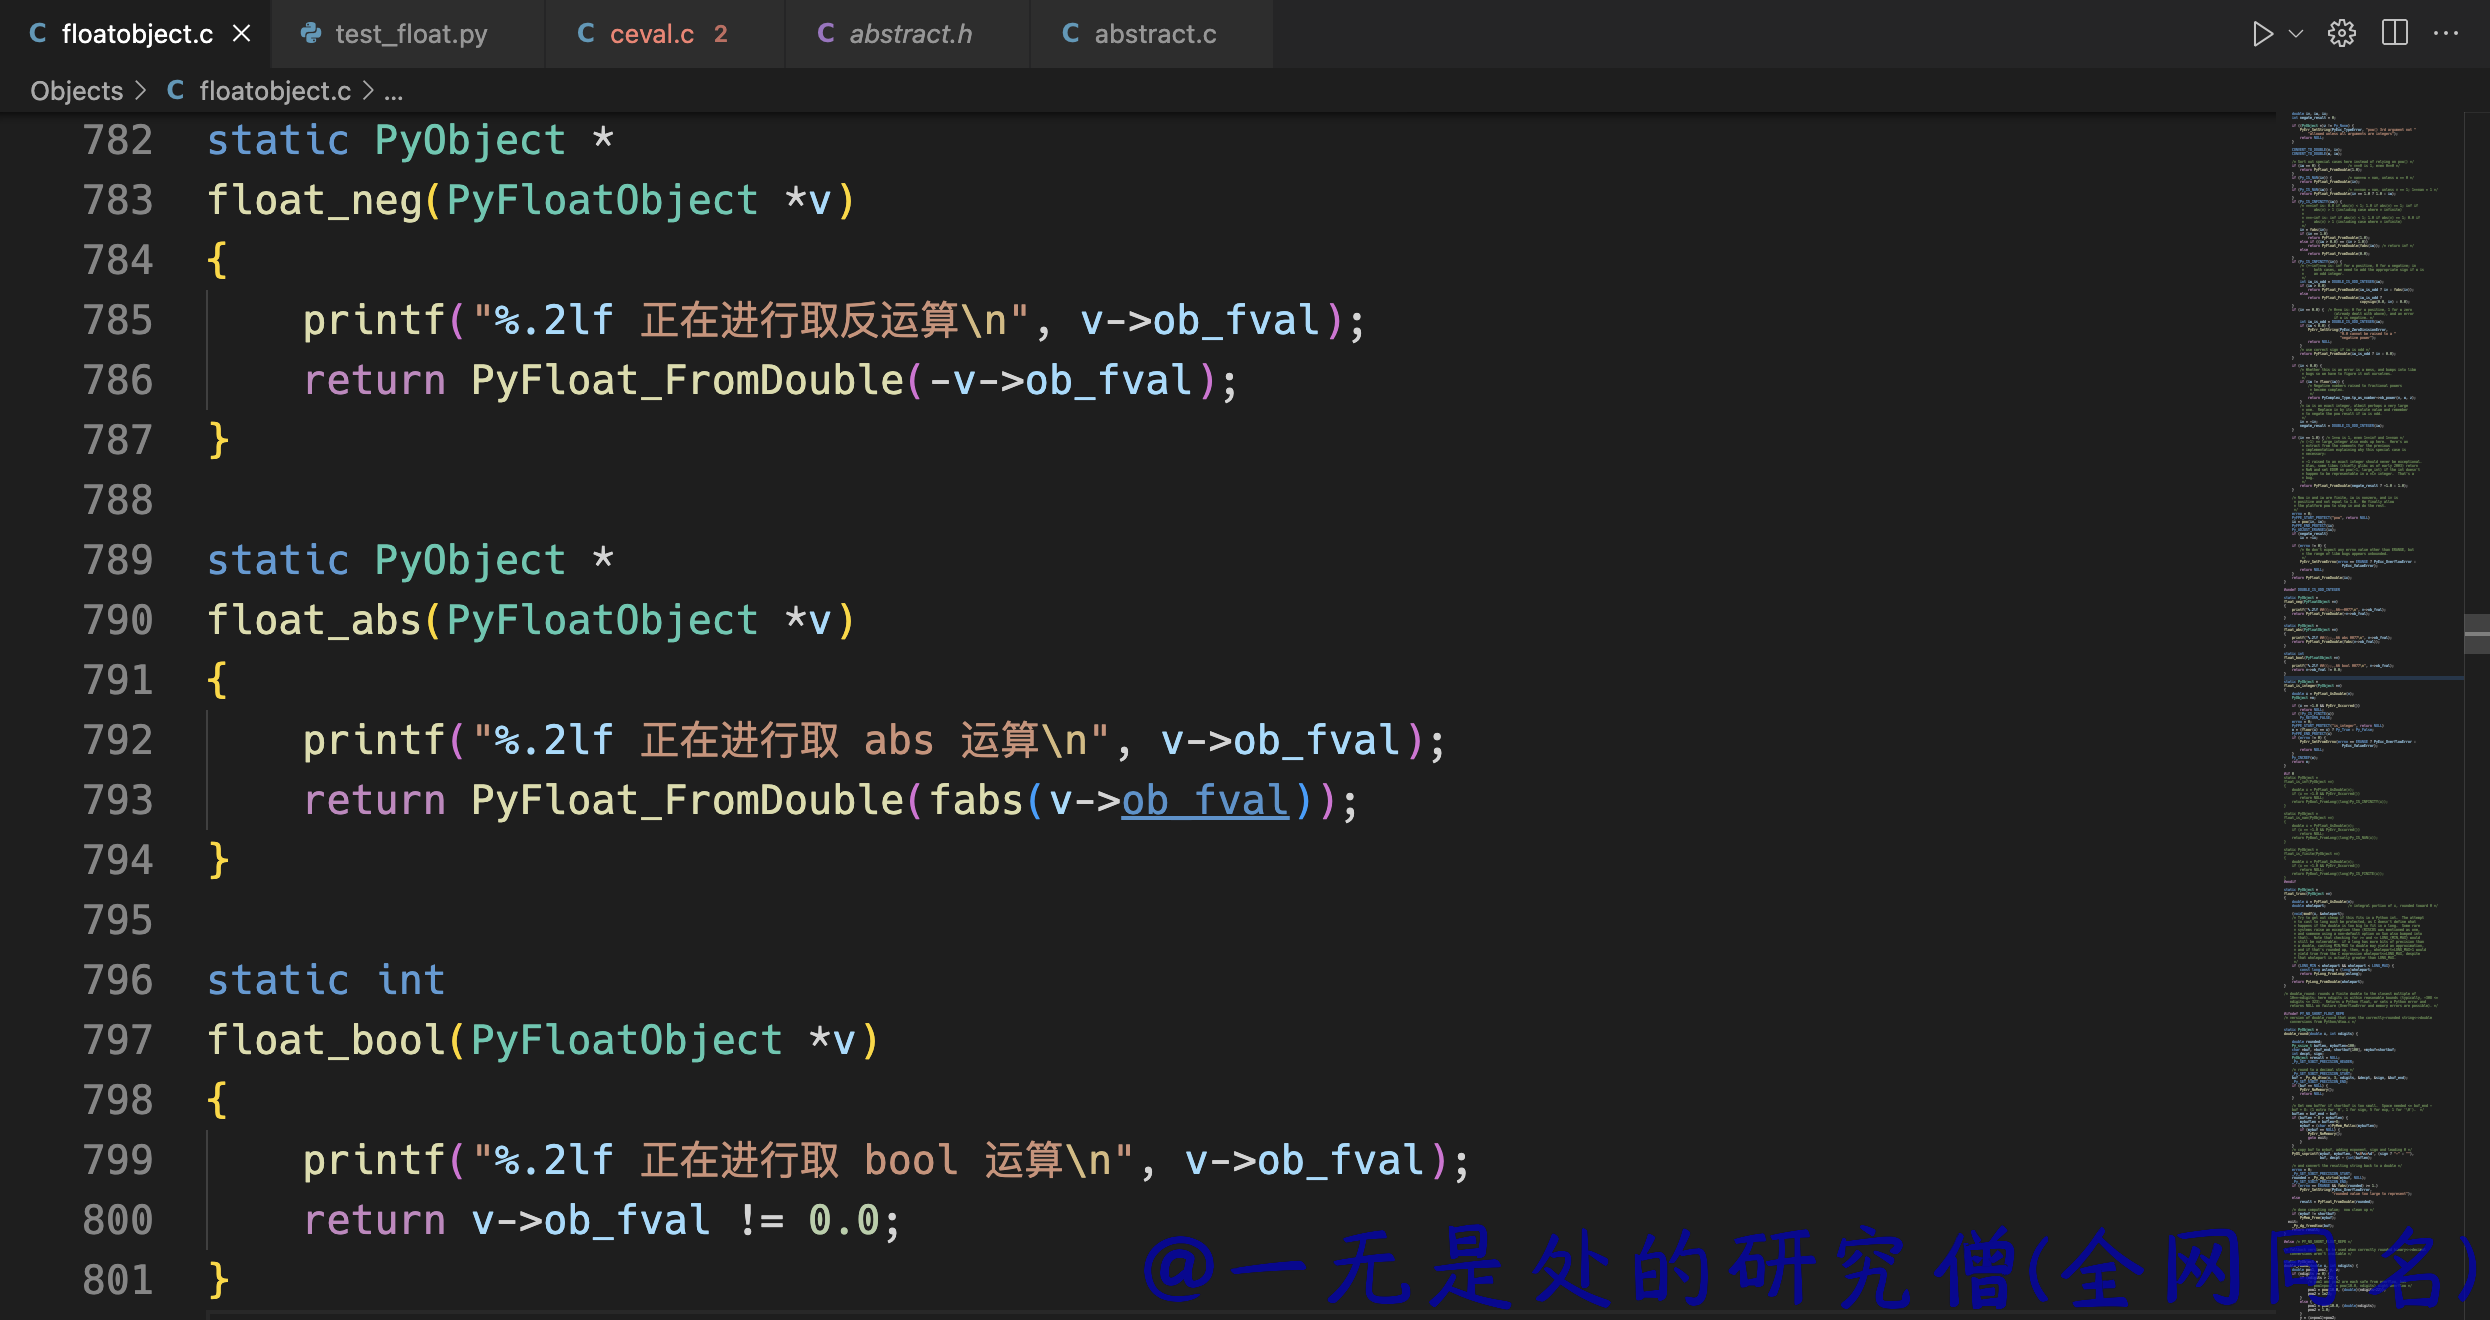
\includegraphics[scale=.12]{images/14-float.png}
            \caption{ }
        \label{fig:my_label}
    \end{figure}
    
下面是修改之后我们再次对浮点数进行操作的时候的输出,可以看到的是输出了我们在上面的代码当中加入的语句。

    \begin{figure}[h]
        \centering
            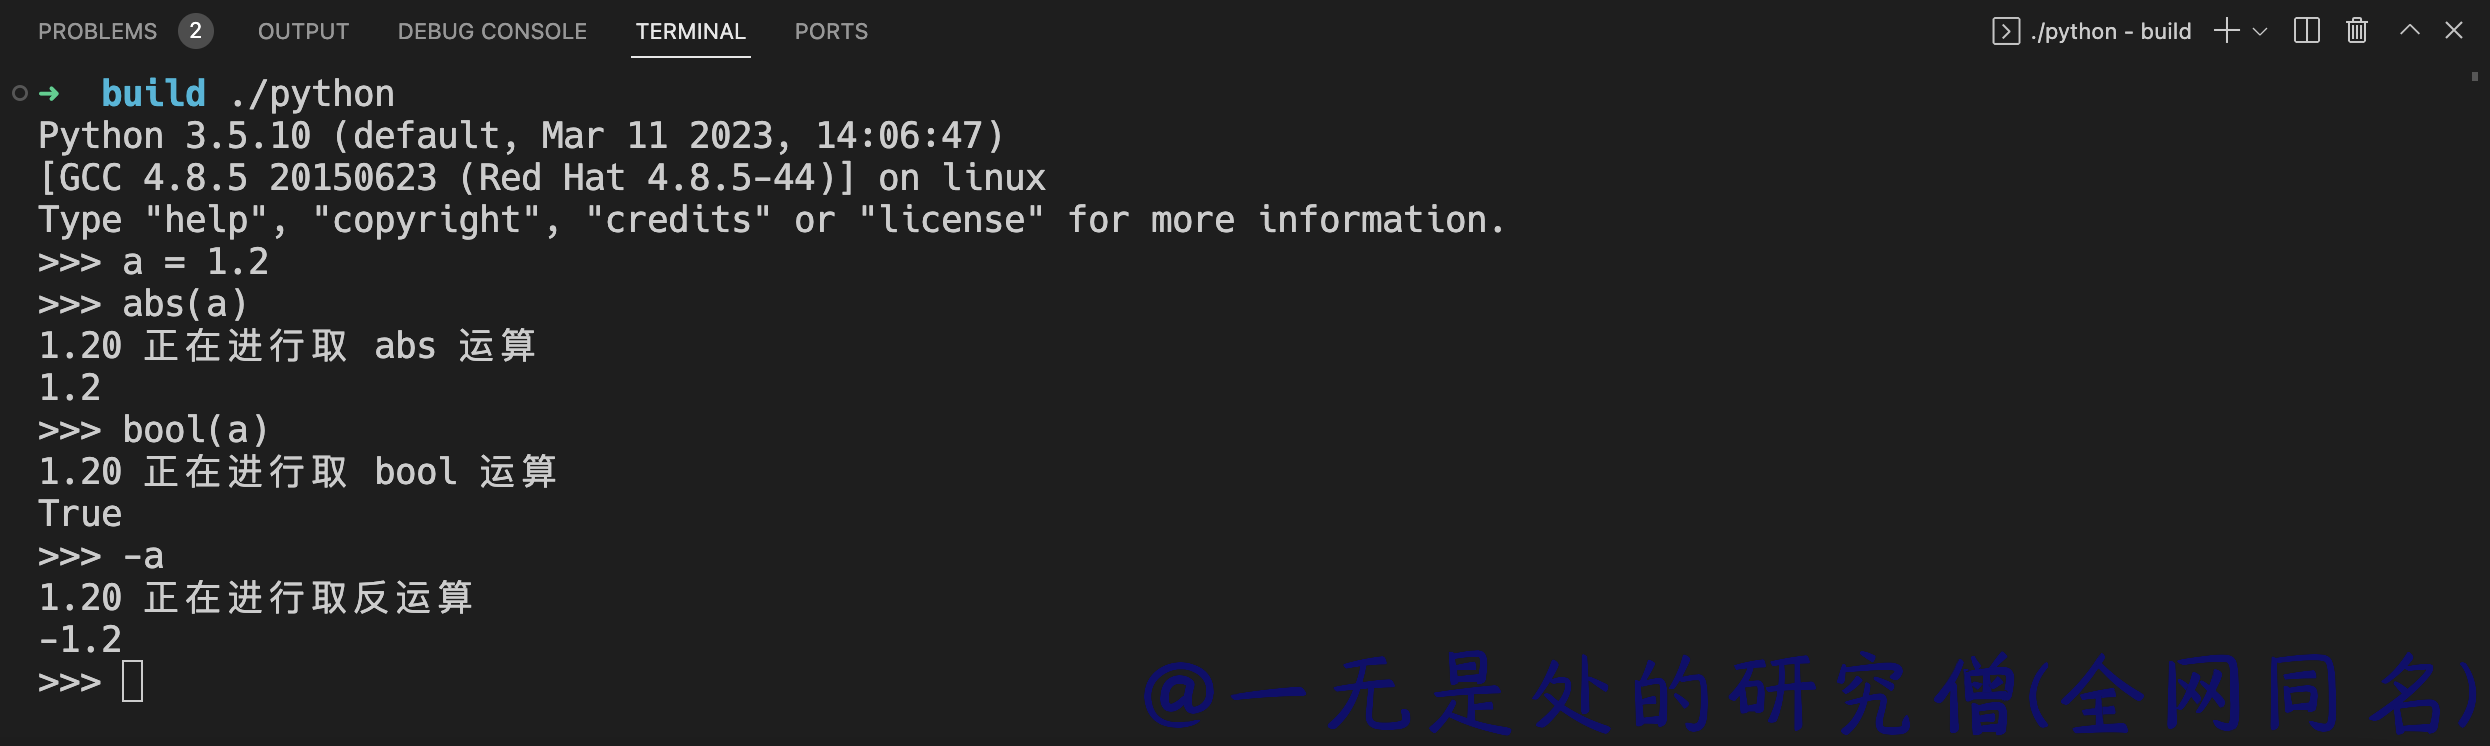
\includegraphics[scale=.2]{images/13-float.png}
            \caption{ }
        \label{fig:my_label}
    \end{figure}
    
\subsection{总结}
在本小节当总主要介绍了一些 float 类型在 cpython 内部是如何实现的以及和他相关的加减乘除方法是如何实现的,以及和部分和关键字有关的函数实现。本小节主要是讨论 float 数据类型本身,不涉及其他的东西,其实关于类型还有非常大一块,就是 cpython 内部对象系统是如何实现的,这一点在后面深入讨论对象系统的时候再进行深入分析,在回头来看 float 类型会有更加深刻的理解。
\section{整型(int)的实现原理及源码剖析}
在本小节当中主要给大家介绍在 cpython 内部是如何实现整型数据 int 的,主要是分析 int 类型的表示方式,分析 int 类型的巧妙设计。
\subsection{数据结构}
在 cpython 内部的 int 类型的实现数据结构如下所示:
\begin{lstlisting}[style=cpp,caption=, language=C++]

typedef struct _longobject PyLongObject;
struct _longobject {
	PyObject_VAR_HEAD
	digit ob_digit[1];
};
#define PyObject_VAR_HEAD      PyVarObject ob_base;
typedef struct {
    PyObject ob_base;
    Py_ssize_t ob_size; /* Number of items in variable part */
} PyVarObject;
typedef struct _object {
    _PyObject_HEAD_EXTRA
    Py_ssize_t ob_refcnt;
    struct _typeobject *ob_type;
} PyObject;
\end{lstlisting}
上面的数据结构用图的方式表示出来如下图所示:

    \begin{figure}[h]
        \centering
            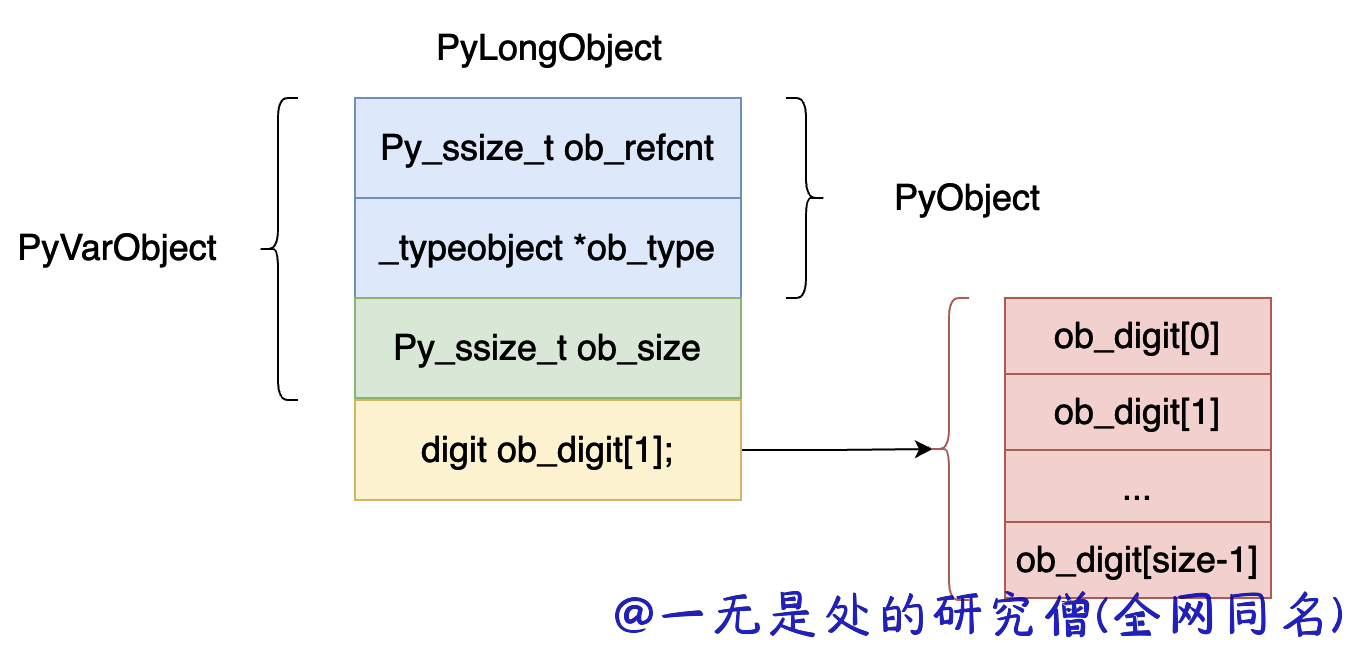
\includegraphics[scale=.2]{images/22-int.png}
            \caption{ }
        \label{fig:my_label}
    \end{figure}
    
\begin{itemize}
\item ob\_refcnt,表示对象的引用记数的个数,这个对于垃圾回收很有用处,后面我们分析虚拟机中垃圾回收部分在深入分析。 
\item ob\_type,表示这个对象的数据类型是什么,在 python 当中有时候需要对数据的数据类型进行判断比如 isinstance, type 这两个关键字就会使用到这个字段。 
\item ob\_size,这个字段表示这个整型对象数组 ob\_digit 当中一共有多少个元素。 
\item digit 类型其实就是 uint32\_t 类型的一个 宏定义,表示 32 位的整型数据。 
\end{itemize}
\subsection{深入分析 PyLongObject 字段的语意}
首先我们知道在 python 当中的整数是不会溢出的,这正是 PyLongObject 使用数组的原因。在 cpython 内部的实现当中,整数有 0 、正数、负数,对于这一点在 cpython 当中有以下几个规定:
\begin{itemize}
\item ob\_size,保存的是数组的长度,ob\_size 大于 0 时保存的是正数,当 ob\_size 小于 0 时保存的是负数。 
\item ob\_digit,保存的是整数的绝对值。在前面我们谈到了,ob\_digit 是一个 32 位的数据,但是在 cpython 内部只会使用其中的前 30 位,这只为了避免溢出的问题。 
\end{itemize}
我们下面使用几个例子来深入理解一下上面的规则:

    \begin{figure}[h]
        \centering
            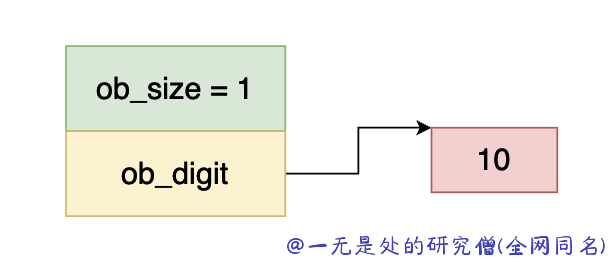
\includegraphics[scale=.3]{images/16-int.png}
            \caption{ }
        \label{fig:my_label}
    \end{figure}
    
在上图当中 ob\_size  大于 0 ,说明这个数是一个正数,而 ob\_digit 指向一个 int32 的数据,数的值等于 10,因此上面这个数表示整数 10 。

    \begin{figure}[h]
        \centering
            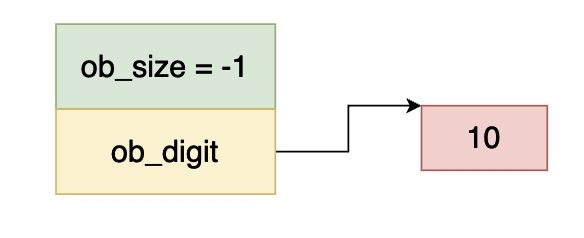
\includegraphics[scale=.3]{images/17-int.png}
            \caption{ }
        \label{fig:my_label}
    \end{figure}
    
同理 ob\_size 小于 0,而 ob\_digit 等于 10,因此上图当中的数据表示 -10 。

    \begin{figure}[h]
        \centering
            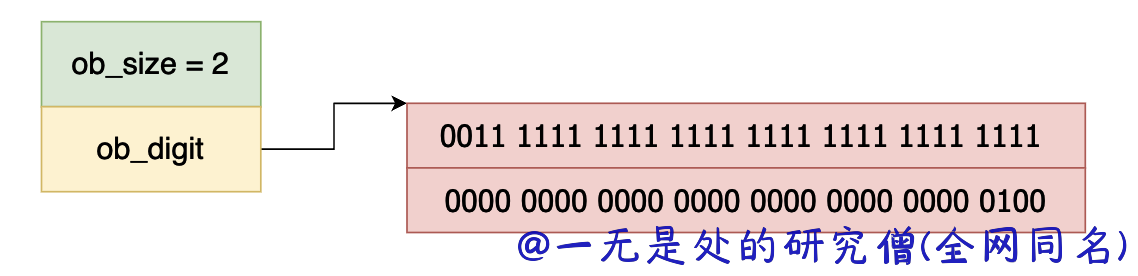
\includegraphics[scale=.3]{images/18-int.png}
            \caption{ }
        \label{fig:my_label}
    \end{figure}
    
上面是一个 ob\_digit 数组长度为 2 的例子,上面所表示数据如下所示:
$$
1 \cdot2^0 + 1 \cdot2^1 + 1 \cdot2^2 + ... + 1 \cdot2^{29} + 0 \cdot2^{30} + 0 \cdot2^{31} + 1 \cdot2^{32}
$$
因为对于每一个数组元素来说我们只使用前 30 位,因此到第二个整型数据的时候正好对应着 $2^{30}$,大家可以对应着上面的结果了解整个计算过程。

    \begin{figure}[h]
        \centering
            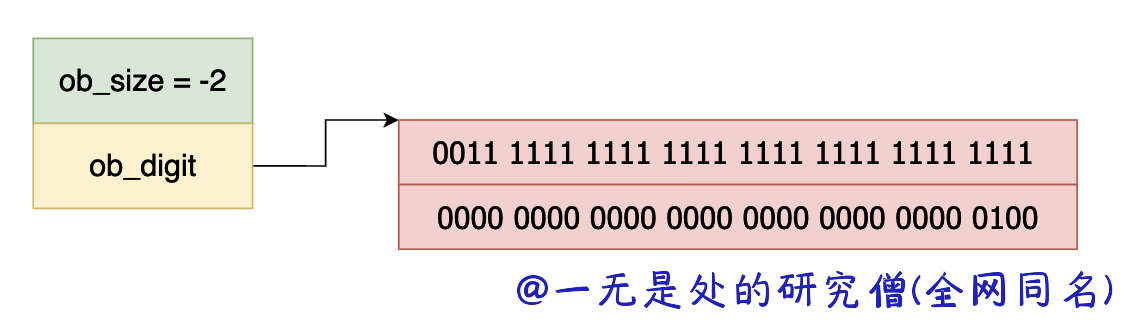
\includegraphics[scale=.3]{images/19-int.png}
            \caption{ }
        \label{fig:my_label}
    \end{figure}
    
上面也就很简单了:
$$
-(1 \cdot2^0 + 1 \cdot2^1 + 1 \cdot2^2 + ... + 1 \cdot2^{29} + 0 \cdot2^{30} + 0 \cdot2^{31} + 1 \cdot2^{32})
$$
\subsection{小整数池}
为了避免频繁的创建一些常用的整数,加快程序执行的速度,我们可以将一些常用的整数先缓存起来,如果需要的话就直接将这个数据返回即可。在 cpython 当中相关的代码如下所示:(小整数池当中缓存数据的区间为[-5, 256])
\begin{lstlisting}[style=cpp,caption=, language=C++]

#define NSMALLPOSINTS           257
#define NSMALLNEGINTS           5
static PyLongObject small_ints[NSMALLNEGINTS + NSMALLPOSINTS];
\end{lstlisting}

    \begin{figure}[h]
        \centering
            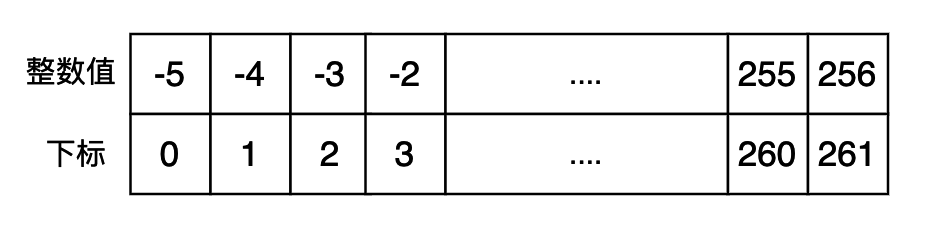
\includegraphics[scale=.3]{images/20-int.png}
            \caption{ }
        \label{fig:my_label}
    \end{figure}
    
我们使用下面的代码进行测试,看是否使用了小整数池当中的数据,如果使用的话,对于使用小整数池当中的数据,他们的 id() 返回值是一样的,id 这个内嵌函数返回的是 python 对象的内存地址。
\begin{lstlisting}[style=py,caption=, language=Python]

>>> a = 1
>>> b = 2
>>> c = 1
>>> id(a), id(c)
(4343136496, 4343136496)
>>> a = -6
>>> c = -6
>>> id(a), id(c)
(4346020624, 4346021072)
>>> a = 257
>>> b = 257
>>> id(a), id(c)
(4346021104, 4346021072)
>>>
\end{lstlisting}
从上面的结果我们可以看到的是,对于区间[-5, 256]当中的值,id 的返回值确实是一样的,不在这个区间之内的返回值就是不一样的。
我们还可以这个特性实现一个小的 trick,就是求一个 PyLongObject 对象所占的内存空间大小,因为我们可以使用 -5 和 256 这两个数据的内存首地址,然后将这个地址相减就可以得到 261 个 PyLongObject 所占的内存空间大小(注意虽然小整数池当中一共有 262 个数据,但是最后一个数据是内存首地址,并不是尾地址,因此只有 261 个数据),这样我们就可以求一个 PyLongObject 对象的内存大小。
\begin{lstlisting}[style=py,caption=, language=Python]

>>> a = -5
>>> b = 256
>>> (id(b) _mmid(a)) / 261 
32.0
>>>
\end{lstlisting}
从上面的输出结果我们可以看到一个 PyLongObject 对象占 32 个字节。我们可以使用下面的 C 程序查看一个 PyLongObject 真实所占的内存空间大小。
\begin{lstlisting}[style=cpp,caption=, language=C++]

#include "Python.h"
#include <stdio.h>
int main()
{
  printf("%ld\n", sizeof(PyLongObject));
  return 0;
}
\end{lstlisting}
上面的程序的输出结果如下所示:

    \begin{figure}[h]
        \centering
            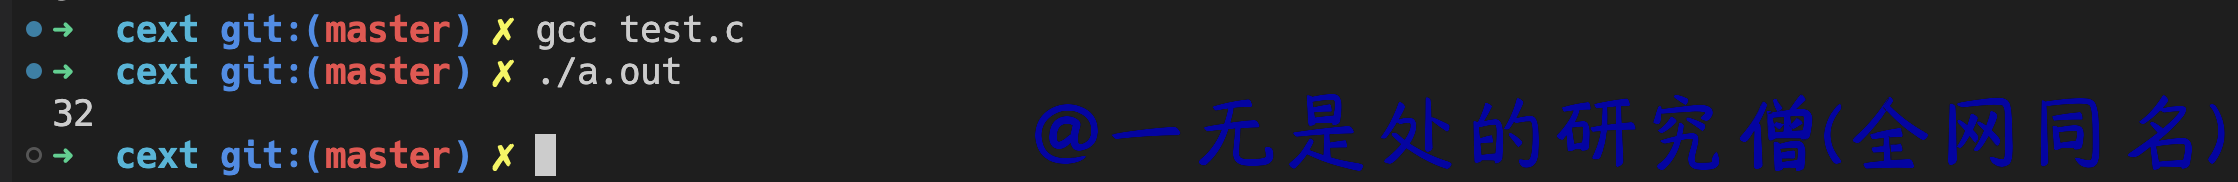
\includegraphics[scale=.2]{images/21-int.png}
            \caption{ }
        \label{fig:my_label}
    \end{figure}
    
上面两个结果是相等的,因此也验证了我们的想法。
从小整数池当中获取数据的核心代码如下所示:
\begin{lstlisting}[style=cpp,caption=, language=C++]

static PyObject *
get_small_int(sdigit ival)
{
    PyObject *v;
    assert(-NSMALLNEGINTS <= ival && ival < NSMALLPOSINTS);
    v = (PyObject *)&small_ints[ival + NSMALLNEGINTS];
    Py_INCREF(v);
    return v;
}
\end{lstlisting}
\subsection{整数的加法实现}
关于 PyLongObject 的操作有很多,我们看一下加法的实现,见微知著,剩下的其他的方法我们就不介绍了,大家感兴趣可以去看具体的源代码。
如果你了解过大整数加法就能够知道,大整数加法的具体实现过程了,在 cpython 内部的实现方式其实也是一样的,就是不断的进行加法操作然后进行进位操作。
\begin{lstlisting}[style=cpp,caption=, language=C++]

#define Py_ABS(x) ((x) < 0 ? -(x) : (x)) // 返回 x 的绝对值
#define PyLong_BASE	((digit)1 << PyLong_SHIFT)
#define PyLong_MASK	((digit)(PyLong_BASE - 1))
static PyLongObject *
x_add(PyLongObject *a, PyLongObject *b)
{
    // 首先获得两个整型数据的 size 
    Py_ssize_t size_a = Py_ABS(Py_SIZE(a)), size_b = Py_ABS(Py_SIZE(b));
    PyLongObject *z;
    Py_ssize_t i;
    digit carry = 0;
    // 确保 a 保存的数据 size 是更大的
    /* Ensure a is the larger of the two: */
    if (size_a < size_b) {
        { PyLongObject *temp = a; a = b; b = temp; }
        { Py_ssize_t size_temp = size_a;
            size_a = size_b;
            size_b = size_temp; }
    }
    // 创建一个新的 PyLongObject 对象,而且数组的长度是 size_a + 1
    z = _PyLong_New(size_a+1);
    if (z == NULL)
        return NULL;
    // 下面就是整个加法操作的核心
    for (i = 0; i < size_b; ++i) {
        carry += a->ob_digit[i] + b->ob_digit[i];
        // 将低 30 位的数据保存下来
        z->ob_digit[i] = carry & PyLong_MASK;
        // 将 carry 右移 30 位,如果上面的加法有进位的话 刚好可以在下一次加法当中使用(注意上面的 carry)
        // 使用的是 += 而不是 =
        carry >>= PyLong_SHIFT; // PyLong_SHIFT = 30
    }
    // 将剩下的长度保存 (因为 a 的 size 是比 b 大的)
    for (; i < size_a; ++i) {
        carry += a->ob_digit[i];
        z->ob_digit[i] = carry & PyLong_MASK;
        carry >>= PyLong_SHIFT;
    }
    // 最后保存高位的进位
    z->ob_digit[i] = carry;
    return long_normalize(z); // long_normalize 这个函数的主要功能是保证 ob_size 保存的是真正的数据的长度 因为可以是一个正数加上一个负数 size 还变小了
}
PyLongObject *
_PyLong_New(Py_ssize_t size)
{
    PyLongObject *result;
    /* Number of bytes needed is: offsetof(PyLongObject, ob_digit) +
       sizeof(digit)*size.  Previous incarnations of this code used
       sizeof(PyVarObject) instead of the offsetof, but this risks being
       incorrect in the presence of padding between the PyVarObject header
       and the digits. */
    if (size > (Py_ssize_t)MAX_LONG_DIGITS) {
        PyErr_SetString(PyExc_OverflowError,
                        "too many digits in integer");
        return NULL;
    }
    // offsetof 会调用 gcc 的一个内嵌函数 __builtin_offsetof 
    // offsetof(PyLongObject, ob_digit)  这个功能是得到 PyLongObject 对象 字段 ob_digit 之前的所有字段所占的内存空间的大小
    result = PyObject_MALLOC(offsetof(PyLongObject, ob_digit) +
                             size*sizeof(digit));
    if (!result) {
        PyErr_NoMemory();
        return NULL;
    }
    // 将对象的 result 的引用计数设置成 1
    return (PyLongObject*)PyObject_INIT_VAR(result, &PyLong_Type, size);
}
static PyLongObject *
long_normalize(PyLongObject *v)
{
    Py_ssize_t j = Py_ABS(Py_SIZE(v));
    Py_ssize_t i = j;
    while (i > 0 && v->ob_digit[i-1] == 0)
        --i;
    if (i != j)
        Py_SIZE(v) = (Py_SIZE(v) < 0) ? -(i) : i;
    return v;
}
\end{lstlisting}
\subsection{总结}
在本小节当中主要给大家介绍了 cpython 内部是如何实现整型数据 int 的,分析了 int 类型的表示方式和设计。int 内部使用 digit 来表示 32 位的整型数据,同时为了避免溢出的问题,只会使用其中的前 30 位。在 cpython 内部的实现当中,整数有 0 、正数、负数,对于这一点有以下几个规定:
\begin{itemize}
\item ob\_size,保存的是数组的长度,ob\_size 大于 0 时保存的是正数,当 ob\_size 小于 0 时保存的是负数。 
\item ob\_digit,保存的是整数的绝对值。 
\item 此外,为避免频繁创建一些常用的整数,cpython 使用了小整数池的技术,将一些常用的整数先缓存起来。最后,本文还介绍了整数的加法实现,即不断进行加法操作然后进行进位操作。 
\end{itemize}
cpython 使用这种方式的主要原理就是大整数的加减乘除,本小节主要是介绍了加法操作,大家如果感兴趣可以自行阅读其他的源程序。

\section{字节(bytes)的实现原理及源码剖析}
在本小节当中主要给大家介绍在 cpython 内部,bytes 的实现原理、内存布局以及与 bytes 相关的一个比较重要的优化点—— bytes 的拼接。
\subsection{数据结构}
\begin{lstlisting}[style=cpp,caption=, language=C++]

typedef struct {
    PyObject_VAR_HEAD
    Py_hash_t ob_shash;
    char ob_sval[1];
    /* Invariants:
     *     ob_sval contains space for 'ob_size+1' elements.
     *     ob_sval[ob_size] == 0.
     *     ob_shash is the hash of the string or -1 if not computed yet.
     */
} PyBytesObject;
typedef struct {
    PyObject ob_base;
    Py_ssize_t ob_size; /* Number of items in variable part */
} PyVarObject;
typedef struct _object {
    Py_ssize_t ob_refcnt;
    struct _typeobject *ob_type;
} PyObject;
\end{lstlisting}
上面的数据结构用图示如下所示:

    \begin{figure}[h]
        \centering
            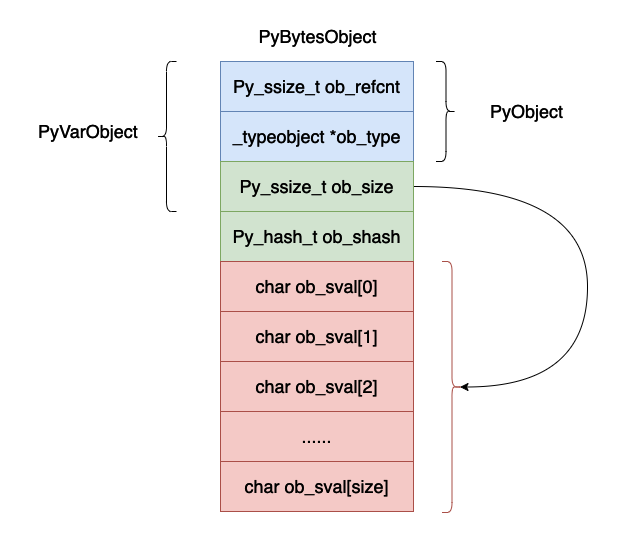
\includegraphics[scale=.25]{images/28-bytes.png}
						\caption{ }
        \label{fig:my_label}
    \end{figure}
    
现在我们来解释一下上面的数据结构各个字段的含义:
\begin{itemize}
\item ob\_refcnt,这个还是对象的引用计数的个数,主要是在垃圾回收的时候有用。 
\item ob\_type,这个是对象的数据类型。 
\item ob\_size,表示这个对象当中字节的个数。 
\item ob\_shash,对象的哈希值,如果还没有计算,哈希值为 -1 。 
\item ob\_sval,一个数据存储一个字节的数据,需要注意的是 ob\_sval[size] 一定等于 \'\\0\' ,表示字符串的结尾。 
\end{itemize}
可能你会有疑问上面的结构体当中并没有后面的那么多字节啊,数组只有一个字节的数据啊,这是因为在 cpython 的实现当中除了申请 PyBytesObject 大的小内存空间之外,还会在这个基础之上申请连续的额外的内存空间用于保存数据,在后续的源码分析当中可以看到这一点。
下面我们举几个例子来说明一下上面的布局:

    \begin{figure}[h]
        \centering
            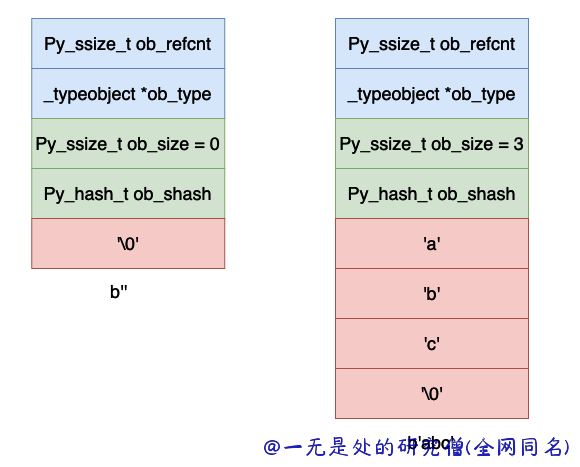
\includegraphics[scale=.25]{images/29-bytes.png}
						\caption{ }
        \label{fig:my_label}
    \end{figure}
    
上面是空和字符串 abc 的字节表示。
\subsection{创建字节对象}
下面是在 cpython 当中通过字节数创建 PyBytesObject 对象的函数。下面的函数的主要功能是创建一个能够存储 size 个字节大小的数据的 PyBytesObject 对象,下面的函数最重要的一个步骤就是申请内存空间。
\begin{lstlisting}[style=cpp,caption=, language=C++]

static PyObject *
_PyBytes_FromSize(Py_ssize_t size, int use_calloc)
{
    PyBytesObject *op;
    assert(size >= 0);
    if (size == 0 && (op = nullstring) != NULL) {
#ifdef COUNT_ALLOCS
        null_strings++;
#endif
        Py_INCREF(op);
        return (PyObject *)op;
    }
    if ((size_t)size > (size_t)PY_SSIZE_T_MAX _mmPyBytesObject_SIZE) { 
        PyErr_SetString(PyExc_OverflowError,
                        "byte string is too large");
        return NULL;
    }
    /* Inline PyObject_NewVar */
    // PyBytesObject_SIZE + size 就是实际申请的内存空间的大小 PyBytesObject_SIZE 就是表示 PyBytesObject 各个字段占用的实际的内存空间大小
    if (use_calloc)
        op = (PyBytesObject *)PyObject_Calloc(1, PyBytesObject_SIZE + size);
    else
        op = (PyBytesObject *)PyObject_Malloc(PyBytesObject_SIZE + size);
    if (op == NULL)
        return PyErr_NoMemory();
    // 将对象的 ob_size 字段赋值成 size 
    (void)PyObject_INIT_VAR(op, &PyBytes_Type, size);
    // 由于对象的哈希值还没有进行计算 因此现将哈希值赋值成 -1
    op->ob_shash = -1;
    if (!use_calloc)
        op->ob_sval[size] = '\0';
    /* empty byte string singleton */
    if (size == 0) {
        nullstring = op;
        Py_INCREF(op);
    }
    return (PyObject *) op;
}
\end{lstlisting}
我们可以使用一个写例子来看一下实际的 PyBytesObject 内存空间的大小。
\begin{lstlisting}[style=py,caption=, language=Python]

>>> import sys
>>> a = b"hello world"
>>> sys.getsizeof(a)
44
>>>
\end{lstlisting}
上面的 44 = 32 + 11 + 1 。
其中 32 是 PyBytesObject 4 个字段所占用的内存空间,ob\_refcnt、ob\_type、ob\_size和 ob\_shash 各占 8 个字节。11 是表示字符串 "hello world" 占用 11 个字节,最后一个字节是 '\\0' 。
\subsection{查看字节长度}
这个函数主要是返回 PyBytesObject 对象的字节长度,也就是直接返回 ob\_size 的值。
\begin{lstlisting}[style=cpp,caption=, language=C++]

static Py_ssize_t
bytes_length(PyBytesObject *a)
{
    // (((PyVarObject*)(ob))->ob_size)
    return Py_SIZE(a);
}
\end{lstlisting}
\subsection{字节拼接}
在 python 当中执行下面的代码就会执行字节拼接函数:
\begin{lstlisting}[style=py,caption=, language=Python]

>>> b"abc" + b"edf"
\end{lstlisting}
下方就是具体的执行字节拼接的函数:
\begin{lstlisting}[style=cpp,caption=, language=C++]

/* This is also used by PyBytes_Concat() */
static PyObject *
bytes_concat(PyObject *a, PyObject *b)
{
    Py_buffer va, vb;
    PyObject *result = NULL;
    va.len = -1;
    vb.len = -1;
    // Py_buffer 当中有一个指针字段 buf 可以用户保存 PyBytesObject 当中字节数据的首地址
    // PyObject_GetBuffer 函数的主要作用是将 对象 a 当中的字节数组赋值给 va 当中的 buf
    if (PyObject_GetBuffer(a, &va, PyBUF_SIMPLE) != 0 ||
        PyObject_GetBuffer(b, &vb, PyBUF_SIMPLE) != 0) {
        PyErr_Format(PyExc_TypeError, "can't concat %.100s to %.100s",
                     Py_TYPE(b)->tp_name, Py_TYPE(a)->tp_name);
        goto done;
    }
    /* Optimize end cases */
    if (va.len == 0 && PyBytes_CheckExact(b)) {
        result = b;
        Py_INCREF(result);
        goto done;
    }
    if (vb.len == 0 && PyBytes_CheckExact(a)) {
        result = a;
        Py_INCREF(result);
        goto done;
    }
    if (va.len > PY_SSIZE_T_MAX _mmvb.len) { 
        PyErr_NoMemory();
        goto done;
    }
    result = PyBytes_FromStringAndSize(NULL, va.len + vb.len);
    // 下方就是将对象 a b 当中的字节数据拷贝到新的
    if (result != NULL) {
        // PyBytes_AS_STRING 宏定义在下方当中 主要就是使用 PyBytesObject 对象当中的
        // ob_sval 字段 也就是将 buf 数据(也就是 a 或者 b 当中的字节数据)拷贝到 ob_sval当中
        memcpy(PyBytes_AS_STRING(result), va.buf, va.len);
        memcpy(PyBytes_AS_STRING(result) + va.len, vb.buf, vb.len);
    }
  done:
    if (va.len != -1)
        PyBuffer_Release(&va);
    if (vb.len != -1)
        PyBuffer_Release(&vb);
    return result;
}
\end{lstlisting}
\begin{lstlisting}[style=cpp,caption=, language=C++]

#define PyBytes_AS_STRING(op) (assert(PyBytes_Check(op)), \
                                (((PyBytesObject *)(op))->ob_sval))
\end{lstlisting}
我们修改一个这个函数,在其中加入一条打印语句,然后重新编译 python 执行结果如下所示:

    \begin{figure}[h]
        \centering
            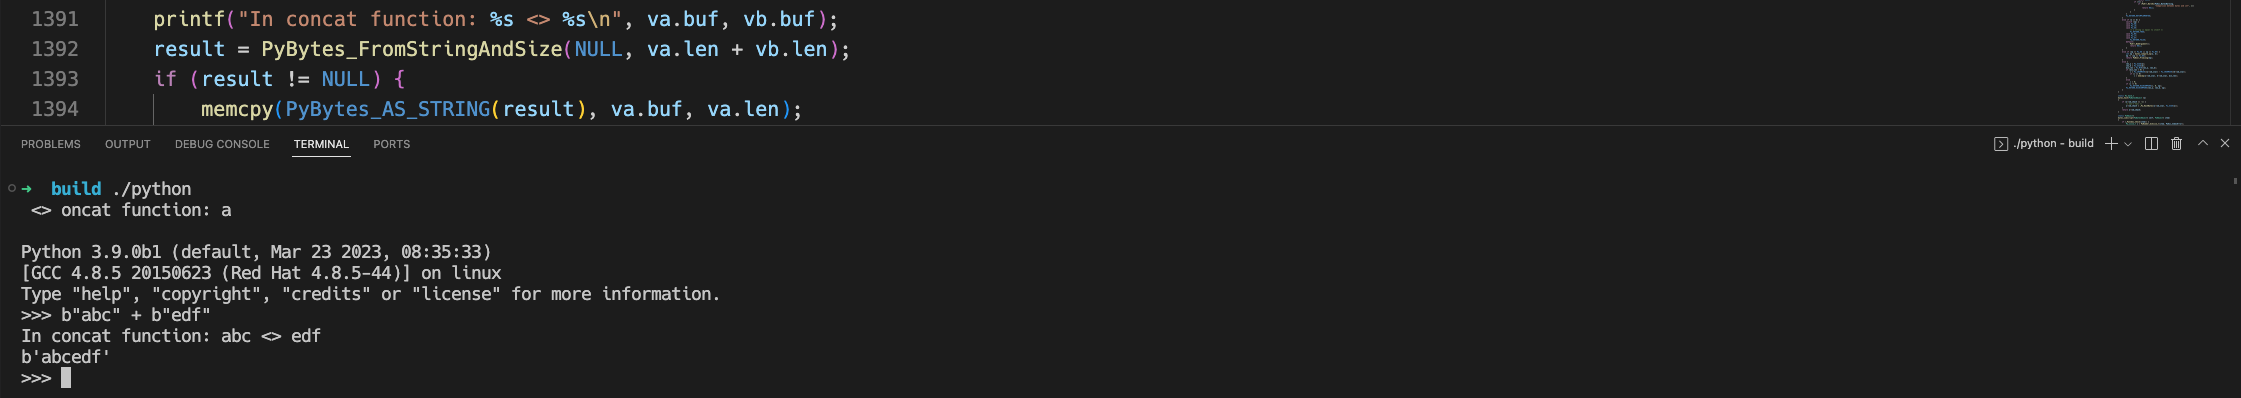
\includegraphics[scale=.2]{images/30-bytes.png}
						\caption{ }
        \label{fig:my_label}
    \end{figure}
    
\begin{lstlisting}[style=py,caption=, language=Python]

Python 3.9.0b1 (default, Mar 23 2023, 08:35:33) 
[GCC 4.8.5 20150623 (Red Hat 4.8.5-44)] on linux
Type "help", "copyright", "credits" or "license" for more information.
>>> b"abc" + b"edf"
In concat function: abc <> edf
b'abcedf'
>>> 
\end{lstlisting}
在上面的拼接函数当中会拷贝原来的两个字节对象,因此需要谨慎使用,一旦发生非常多的拷贝的话是非常耗费内存的。因此需要警惕使用循环内的内存拼接。比如对于 [b"a", b"b", b"c"] 来说,如果使用循环拼接的话,那么会将 b"a" 拷贝两次。
\begin{lstlisting}[style=cpp,caption=, language=C++]

>>> res = b""
>>> for item in  [b"a", b"b", b"c"]:
...     res += item
...
>>> res
b'abc'
>>>
\end{lstlisting}
因为 b"a", b"b" 在拼接的时候会将他们分别拷贝一次,在进行 b"ab",b"c" 拼接的时候又会将 ab 和 c 拷贝一次,那么具体的拷贝情况如下所示:
\begin{itemize}
\item "a" 拷贝了一次。 
\item "b" 拷贝了一次。 
\item "ab" 拷贝了一次。 
\item "c" 拷贝了一次。 
\end{itemize}
但是实际上我们的需求是只需要对 [b"a", b"b", b"c"] 当中的数据各拷贝一次,如果我们要实现这一点可以使用 b"".join([b"a", b"b", b"c"]),直接将 [b"a", b"b", b"c"] 作为参数传递,然后各自只拷贝一次,具体的实现代码如下所示,在这个例子当中 sep 就是空串 b"",iterable 就是 [b"a", b"b", b"c"] 。
\begin{lstlisting}[style=cpp,caption=, language=C++]

Py_LOCAL_INLINE(PyObject *)
STRINGLIB(bytes_join)(PyObject *sep, PyObject *iterable)
{
    char *sepstr = STRINGLIB_STR(sep);
    const Py_ssize_t seplen = STRINGLIB_LEN(sep);
    PyObject *res = NULL;
    char *p;
    Py_ssize_t seqlen = 0;
    Py_ssize_t sz = 0;
    Py_ssize_t i, nbufs;
    PyObject *seq, *item;
    Py_buffer *buffers = NULL;
#define NB_STATIC_BUFFERS 10
    Py_buffer static_buffers[NB_STATIC_BUFFERS];
    seq = PySequence_Fast(iterable, "can only join an iterable");
    if (seq == NULL) {
        return NULL;
    }
    seqlen = PySequence_Fast_GET_SIZE(seq);
    if (seqlen == 0) {
        Py_DECREF(seq);
        return STRINGLIB_NEW(NULL, 0);
    }
#ifndef STRINGLIB_MUTABLE
    if (seqlen == 1) {
        item = PySequence_Fast_GET_ITEM(seq, 0);
        if (STRINGLIB_CHECK_EXACT(item)) {
            Py_INCREF(item);
            Py_DECREF(seq);
            return item;
        }
    }
#endif
    if (seqlen > NB_STATIC_BUFFERS) {
        buffers = PyMem_NEW(Py_buffer, seqlen);
        if (buffers == NULL) {
            Py_DECREF(seq);
            PyErr_NoMemory();
            return NULL;
        }
    }
    else {
        buffers = static_buffers;
    }
    /* Here is the general case.  Do a pre-pass to figure out the total
     * amount of space we'll need (sz), and see whether all arguments are
     * bytes-like.
     */
    for (i = 0, nbufs = 0; i < seqlen; i++) {
        Py_ssize_t itemlen;
        item = PySequence_Fast_GET_ITEM(seq, i);
        if (PyBytes_CheckExact(item)) {
            /* Fast path. */
            Py_INCREF(item);
            buffers[i].obj = item;
            buffers[i].buf = PyBytes_AS_STRING(item);
            buffers[i].len = PyBytes_GET_SIZE(item);
        }
        else if (PyObject_GetBuffer(item, &buffers[i], PyBUF_SIMPLE) != 0) {
            PyErr_Format(PyExc_TypeError,
                         "sequence item %zd: expected a bytes-like object, "
                         "%.80s found",
                         i, Py_TYPE(item)->tp_name);
            goto error;
        }
        nbufs = i + 1;  /* for error cleanup */
        itemlen = buffers[i].len;
        if (itemlen > PY_SSIZE_T_MAX _mmsz) { 
            PyErr_SetString(PyExc_OverflowError,
                            "join() result is too long");
            goto error;
        }
        sz += itemlen;
        if (i != 0) {
            if (seplen > PY_SSIZE_T_MAX _mmsz) { 
                PyErr_SetString(PyExc_OverflowError,
                                "join() result is too long");
                goto error;
            }
            sz += seplen;
        }
        if (seqlen != PySequence_Fast_GET_SIZE(seq)) {
            PyErr_SetString(PyExc_RuntimeError,
                            "sequence changed size during iteration");
            goto error;
        }
    }
    /* Allocate result space. */
    res = STRINGLIB_NEW(NULL, sz);
    if (res == NULL)
        goto error;
    /* Catenate everything. */
    p = STRINGLIB_STR(res);
    if (!seplen) {
        /* fast path */
        for (i = 0; i < nbufs; i++) {
            Py_ssize_t n = buffers[i].len;
            char *q = buffers[i].buf;
            Py_MEMCPY(p, q, n);
            p += n;
        }
        goto done;
    }
    // 具体的实现逻辑就是在这里
    for (i = 0; i < nbufs; i++) {
        Py_ssize_t n;
        char *q;
        if (i) {
            // 首先现将 sepstr 拷贝到新的数组里面但是在我们举的例子当中是空串 b""
            Py_MEMCPY(p, sepstr, seplen);
            p += seplen;
        }
        n = buffers[i].len;
        q = buffers[i].buf;
        // 然后将列表当中第 i 个 bytes 的数据拷贝到 p 当中 这样就是实现了我们所需要的效果
        Py_MEMCPY(p, q, n);
        p += n;
    }
    goto done;
error:
    res = NULL;
done:
    Py_DECREF(seq);
    for (i = 0; i < nbufs; i++)
        PyBuffer_Release(&buffers[i]);
    if (buffers != static_buffers)
        PyMem_FREE(buffers);
    return res;
}
\end{lstlisting}
\subsection{单字节字符}
在 cpython 的内部实现当中给单字节的字符做了一个小的缓冲池:
\begin{lstlisting}[style=cpp,caption=, language=C++]

static PyBytesObject *characters[UCHAR_MAX + 1]; // UCHAR_MAX 在 64 位系统当中等于 255
\end{lstlisting}
当创建的 bytes 只有一个字符的时候就可以检查是否 characters 当中已经存在了,如果存在就直接返回这个已经创建好的 PyBytesObject 对象,否则再进行创建。新创建的 PyBytesObject 对象如果长度等于 1 的话也会被加入到这个数组当中。下面是 PyBytesObject 的另外一个创建函数:
\begin{lstlisting}[style=cpp,caption=, language=C++]

PyObject *
PyBytes_FromStringAndSize(const char *str, Py_ssize_t size)
{
    PyBytesObject *op;
    if (size < 0) {
        PyErr_SetString(PyExc_SystemError,
            "Negative size passed to PyBytes_FromStringAndSize");
        return NULL;
    }
    // 如果创建长度等于 1 而且对象在 characters 当中存在的话那么就直接返回
    if (size == 1 && str != NULL &&
        (op = characters[*str & UCHAR_MAX]) != NULL)
    {
#ifdef COUNT_ALLOCS
        one_strings++;
#endif
        Py_INCREF(op);
        return (PyObject *)op;
    }
    op = (PyBytesObject *)_PyBytes_FromSize(size, 0);
    if (op == NULL)
        return NULL;
    if (str == NULL)
        return (PyObject *) op;
    Py_MEMCPY(op->ob_sval, str, size);
    /* share short strings */
    // 如果创建的对象的长度等于 1 那么久将这个对象保存到 characters 当中
    if (size == 1) {
        characters[*str & UCHAR_MAX] = op;
        Py_INCREF(op);
    }
    return (PyObject *) op;
}
\end{lstlisting}
我们可以使用下面的代码进行验证:
\begin{lstlisting}[style=py,caption=, language=Python]

>>> a = b"a"
>>> b  =b"a"
>>> a == b
True
>>> a is b
True
>>> a = b"aa"
>>> b = b"aa"
>>> a == b
True
>>> a is b
False
\end{lstlisting}
从上面的代码可以知道,确实当我们创建的 bytes 的长度等于 1 的时候对象确实是同一个对象。
\subsection{总结}
在本小节当中主要给大家介绍了在 cpython 内部对于 bytes 的实现,重点介绍了 cpython 当中 PyBytesObject 的内存布局和创建 PyBytesObject 的函数,以及对于 bytes 对象的拼接细节和 cpython 内部单字节字符的缓冲池。在程序当中最好使用 join 操作进行 btyes 的拼接操作,否则效率会比较低。

\chapter{深入理解程序的执行}
\section{pyc 文件结构}
在本小节当中主要给大家介绍一下 .py 文件在被编译之后对应的 pyc 文件结构,pyc 文件当中的一个核心内容就是 python 字节码。
\subsection{pyc 文件}
pyc 文件是 Python 在解释执行源代码时生成的一种字节码文件,它包含了源代码的编译结果和相关的元数据信息,以便于 Python 可以更快地加载和执行代码。
Python 是一种解释型语言,它不像编译型语言那样将源代码直接编译成机器码执行。Python 的解释器会在运行代码之前先将源代码编译成字节码,然后将字节码解释执行。.pyc 文件就是这个过程中生成的字节码文件。
当 Python 解释器首次执行一个 .py 文件时,它会在同一目录下生成一个对应的 .pyc 文件,以便于下次加载该文件时可以更快地执行。如果源文件在修改之后被重新加载,解释器会重新生成 .pyc 文件以更新缓存的字节码。
\subsection{生成 pyc 文件}
正常的 python 文件需要通过编译器变成字节码,然后将字节码交给 python 虚拟机,然后 python 虚拟机会执行字节码。整体流程如下所示:

    \begin{figure}[H]
        \centering
            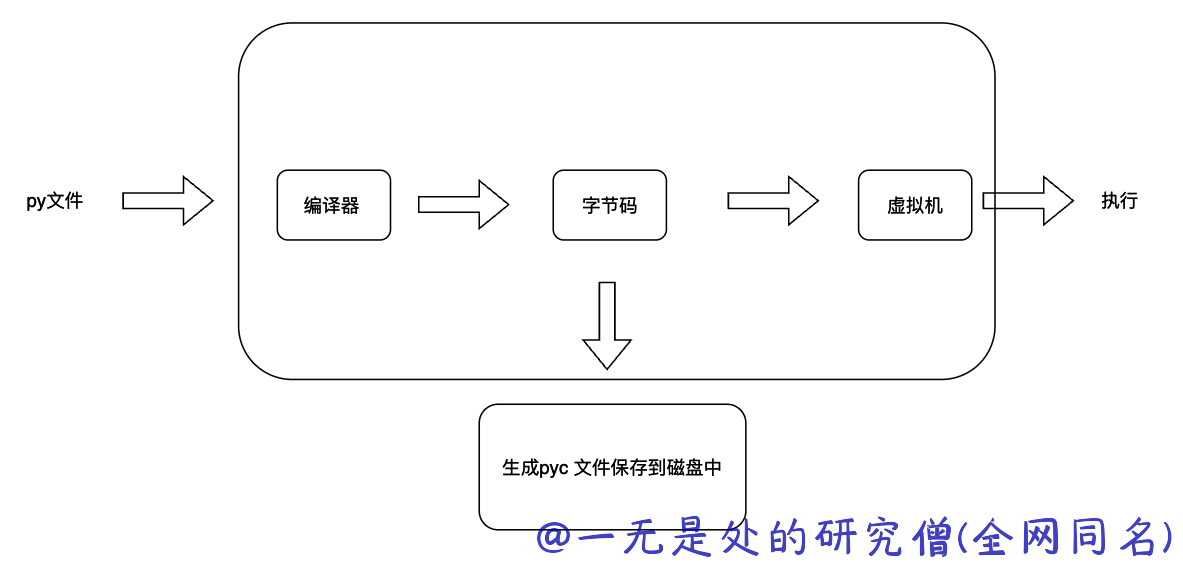
\includegraphics[scale=.25]{images/35-pyc.png}
						\caption{ }
        \label{fig:my_label}
    \end{figure}
    
我们可以直接使用 compile all 模块生成对应文件的 pyc 文件。
\begin{lstlisting}[style=cpp,caption=, language=C++]

➜  pvm ls
demo.py  hello.py
➜  pvm python -m compileall .
Listing '.'...
Listing './.idea'...
Listing './.idea/inspectionProfiles'...
Compiling './demo.py'...
Compiling './hello.py'...
➜  pvm ls
__pycache__ demo.py     hello.py
➜  pvm ls __pycache__ 
demo.cpython-310.pyc  hello.cpython-310.pyc
\end{lstlisting}
\verb|python -m compileall .| 命令将递归扫描当前目录下面的 py 文件,并且生成对应文件的 pyc 文件。
\subsection{pyc 文件布局}

    \begin{figure}[H]
        \centering
            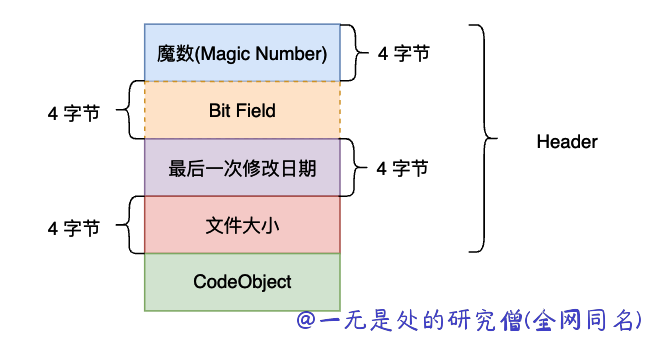
\includegraphics[scale=.35]{images/38-pyc.png}
						\caption{ }
        \label{fig:my_label}
    \end{figure}
    
第一部分魔数由两部分组成:

    \begin{figure}[H]
        \centering
            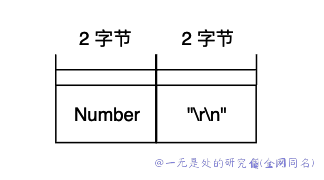
\includegraphics[scale=.3]{images/37-pyc.png}
						\caption{ }
        \label{fig:my_label}
    \end{figure}
第一部分 魔术是由一个 2 字节的整数和另外两个字符回车换行组成的, \verb|"\r\n"|  也占用两个字节,一共是四个字节。这个两个字节的整数在不同的 python 版本还不一样,比如说在 python3.5 当中这个值为 3351 等值,在 python3.9 当中这个值为 3420,3421,3422,3423,3424等值(在 python 3.9 的小版本)。

第二部分 Bit Field 这个字段的主要作用是为了将来能够实现复现编译结果,但是在 python3.9a2 时,这个字段的值还全部是 0 。详细内容可以参考 [PEP552-Deterministic pycs]\footnote{\href{https://peps.python.org/pep-0552/}{https://peps.python.org/pep-0552/}} 。这个字段在 python2 和 python3 早期版本并没有(python3.5 还没有),在 python3 的后期版本这个字段才出现的。

第三部分 就是整个 py  源文件的大小了。

第四部分 也是整个 pyc 文件当中最重要的一个部分,最后一个部分就是一个 CodeObject 对象序列化之后的数据,我们稍后再来仔细分析一下这个对象相关的数据。

我们现在来具体分析一个 pyc 文件,对应的 python 代码为:
\begin{lstlisting}[style=py,caption=, language=Python]

def f():
    x = 1
    return 2
\end{lstlisting}
pyc 文件的十六进制形式如下所示:
\begin{lstlisting}[style=cpp,caption=, language=C++]

➜  __pycache__ hexdump -C hello.cpython-310.pyc
00000000  6f 0d 0d 0a 00 00 00 00  b9 48 21 64 20 00 00 00  |o........H!d ...|
00000010  e3 00 00 00 00 00 00 00  00 00 00 00 00 00 00 00  |................|
00000020  00 02 00 00 00 40 00 00  00 73 0c 00 00 00 64 00  |.....@...s....d.|
00000030  64 01 84 00 5a 00 64 02  53 00 29 03 63 00 00 00  |d...Z.d.S.).c...|
00000040  00 00 00 00 00 00 00 00  00 01 00 00 00 01 00 00  |................|
00000050  00 43 00 00 00 73 08 00  00 00 64 01 7d 00 64 02  |.C...s....d.}.d.|
00000060  53 00 29 03 4e e9 01 00  00 00 e9 02 00 00 00 a9  |S.).N...........|
00000070  00 29 01 da 01 78 72 03  00 00 00 72 03 00 00 00  |.)...xr....r....|
00000080  fa 0a 2e 2f 68 65 6c 6c  6f 2e 70 79 da 01 66 01  |.hello.py..f.|
00000090  00 00 00 73 04 00 00 00  04 01 04 01 72 06 00 00  |...s........r...|
000000a0  00 4e 29 01 72 06 00 00  00 72 03 00 00 00 72 03  |.N).r....r....r.|
000000b0  00 00 00 72 03 00 00 00  72 05 00 00 00 da 08 3c  |...r....r......<|
000000c0  6d 6f 64 75 6c 65 3e 01  00 00 00 73 02 00 00 00  |module>....s....|
000000d0  0c 00                                             |..|
000000d2
\end{lstlisting}
因为数据使用小端表示方式,因此对于上面的数据来说:
\begin{itemize}
\item 第一部分魔数为:0xa0d0d6f 。 
\item 第二部分 Bit Field 为:0x0 。 
\item 第三部分最后一次修改日期为:0x642148b9 。 
\item 第四部分文件大小为:0x20 字节,也就是说 hello.py 这个文件的大小是 32 字节。 
\end{itemize}
下面是一个小的代码片段用于读取 pyc 文件的头部元信息:
\begin{lstlisting}[style=py,caption=, language=Python]

import struct
import time
import binascii
fname = "./__pycache__/hello.cpython-310.pyc"
f = open(fname, "rb")
magic = struct.unpack('<l', f.read(4))[0]
bit_filed = f.read(4)
print(f"bit field = {binascii.hexlify(bit_filed)}")
moddate = f.read(4)
filesz = f.read(4)
modtime = time.asctime(time.localtime(struct.unpack('<l', moddate)[0]))
filesz = struct.unpack('<L', filesz)
print("magic %s" % (hex(magic)))
print("moddate (%s)" % (modtime))
print("File Size %d" % filesz)
f.close()
\end{lstlisting}
上面的代码输出结果如下所示:
\begin{lstlisting}[style=cpp,caption=, language=C++]

bit field = b'00000000'
magic 0xa0d0d6f
moddate (Mon Mar 27 15:41:45 2023)
File Size 32
\end{lstlisting}
有关 pyc 文件的详细操作可以查看 python 标准库 importlib/\_bootstrap\_external.py 文件源代码。
\subsection{CodeObject}
在 CPython 中,\verb|CodeObject| 是一个对象,它包含了 Python 代码的字节码、常量、变量、位置参数、关键字参数等信息,以及一些用于运行代码的元数据,如文件名、代码行号等。
在 CPython 中,当我们执行一个 Python 模块或函数时,解释器会先将其代码编译为 \verb|CodeObject|,然后再执行。在编译过程中,解释器会将 Python 代码转换为字节码,并将其保存在 \verb|CodeObject| 对象中。此后,每当我们调用该模块或函数时,解释器都会使用 \verb|CodeObject| 中的字节码来执行代码。
\verb|CodeObject| 对象是不可变的,一旦创建就不能被修改。这是因为 Python 代码的字节码是不可变的,而 \verb|CodeObject| 对象包含了这些字节码,所以也是不可变的。
在本小节当中主要介绍 code object 当中主要的内容,以及简单介绍他们的作用,在后续的文章当中会仔细分析 code object 对应的源代码以及对应的字段的详细作用。
现在举一个例子来分析一下 pycdemo.py 的 pyc 文件,pycdemo.py 的源程序如下所示:
\begin{lstlisting}[style=py,caption=, language=Python]

if __name__ == '__main__':
    a = 100
    print(a)
\end{lstlisting}
下面的代码是一个用于加载 pycdemo01.cpython-39.pyc 文件(也就是 hello.py 对应的 pyc 文件)的代码,使用 marshal 读取 pyc 文件里面的 code object 。
\begin{lstlisting}[style=py,caption=, language=Python]

import marshal
import dis
import struct
import time
import types
import binascii
def print_metadata(fp):
    magic = struct.unpack('<l', fp.read(4))[0]
    print(f"magic number = {hex(magic)}")
    bit_field = struct.unpack('<l', fp.read(4))[0]
    print(f"bit filed = {bit_field}")
    t = struct.unpack('<l', fp.read(4))[0]
    print(f"time = {time.asctime(time.localtime(t))}")
    file_size = struct.unpack('<l', fp.read(4))[0]
    print(f"file size = {file_size}")
def show_code(code, indent=''):
    print ("%scode" % indent)
    indent += '   '
    print ("%sargcount %d" % (indent, code.co_argcount))
    print ("%snlocals %d" % (indent, code.co_nlocals))
    print ("%sstacksize %d" % (indent, code.co_stacksize))
    print ("%sflags %04x" % (indent, code.co_flags))
    show_hex("code", code.co_code, indent=indent)
    dis.disassemble(code)
    print ("%sconsts" % indent)
    for const in code.co_consts:
        if type(const) == types.CodeType:
            show_code(const, indent+'   ')
        else:
            print("   %s%r" % (indent, const))
    print("%snames %r" % (indent, code.co_names))
    print("%svarnames %r" % (indent, code.co_varnames))
    print("%sfreevars %r" % (indent, code.co_freevars))
    print("%scellvars %r" % (indent, code.co_cellvars))
    print("%sfilename %r" % (indent, code.co_filename))
    print("%sname %r" % (indent, code.co_name))
    print("%sfirstlineno %d" % (indent, code.co_firstlineno))
    show_hex("lnotab", code.co_lnotab, indent=indent)
def show_hex(label, h, indent):
    h = binascii.hexlify(h)
    if len(h) < 60:
        print("%s%s %s" % (indent, label, h))
    else:
        print("%s%s" % (indent, label))
        for i in range(0, len(h), 60):
            print("%s   %s" % (indent, h[i:i+60]))
if __name__ == '__main__':
    filename = "./__pycache__/pycdemo01.cpython-39.pyc"
    with open(filename, "rb") as fp:
        print_metadata(fp)
        code_object = marshal.load(fp)
        show_code(code_object)
\end{lstlisting}
执行上面的程序输出结果如下所示:
\begin{lstlisting}[style=cpp,caption=, language=C++]

magic number = 0xa0d0d61
bit filed = 0
time = Tue Mar 28 02:40:20 2023
file size = 54
code
   argcount 0
   nlocals 0
   stacksize 2
   flags 0040
   code b'650064006b02721464015a01650265018301010064025300'
  3           0 LOAD_NAME                0 (__name__)
              2 LOAD_CONST               0 ('__main__')
              4 COMPARE_OP               2 (==)
              6 POP_JUMP_IF_FALSE       20
  4           8 LOAD_CONST               1 (100)
             10 STORE_NAME               1 (a)
  5          12 LOAD_NAME                2 (print)
             14 LOAD_NAME                1 (a)
             16 CALL_FUNCTION            1
             18 POP_TOP
        >>   20 LOAD_CONST               2 (None)
             22 RETURN_VALUE
   consts
      '__main__'
      100
      None
   names ('__name__', 'a', 'print')
   varnames ()
   freevars ()
   cellvars ()
   filename './pycdemo01.py'
   name '<module>'
   firstlineno 3
   lnotab b'08010401'
\end{lstlisting}
下面是 code object 当中各个字段的作用:
\begin{itemize}
\item 首先需要了解一下代码块这个概念,所谓代码块就是一个小的 python 代码,被当做一个小的单元整体执行。在 python 当中常见的代码块块有:函数体、类的定义、一个模块。 
\item argcount,这个表示一个代码块的参数个数,这个参数只对函数体代码块有用,因为函数可能会有参数,比如上面的 pycdemo.py 是一个模块而不是一个函数,因此这个参数对应的值为 0 。 
\item co\_code,这个对象的具体内容就是一个字节序列,存储真实的 python 字节码,主要是用于 python 虚拟机执行的,在本小节当中暂时不详细分析。 
\item co\_consts,这个字段是一个列表类型的字段,主要是包含一些字符串常量和数值常量,比如上面的 "\_\_main\_\_" 和 100 。 
\item co\_filename,这个字段的含义就是对应的源文件的文件名。 
\item co\_firstlineno,这个字段的含义为在 python 源文件当中第一行代码出现的行数,这个字段在进行调试的时候非常重要。 
\item co\_flags,这个字段的主要含义就是标识这个 code object 的类型。0x0080 表示这个 block 是一个协程,0x0010 表示这个 code object 是嵌套的等等。 
\item co\_lnotab,这个字段的含义主要是用于计算每个字节码指令对应的源代码行数。 
\item co\_varnames,这个字段的主要含义是表示在一个 code object 本地定义的一个名字。 
\item co\_names,和 co\_varnames 相反,表示非本地定义但是在 code object 当中使用的名字。 
\item co\_nlocals,这个字段表示在一个 code object 当中本地使用的变量个数。 
\item co\_stackszie,因为 python 虚拟机是一个栈式计算机,这个参数的值表示这个栈需要的最大的值。 
\item co\_cellvars,co\_freevars,这两个字段主要和嵌套函数和函数闭包有关,我们在后续的文章当中将详细解释这个字段。 
\end{itemize}
\subsection{总结}
在本小节当中主要给大家介绍了 python 文件被编译之后的结果文件 .pyc 文件结构,在 pyc 文件当中一个最重要的结构就是 code object 对象,在本小节当中主要是简单介绍了 code object 各个字段的作用。在后续的文章当中将会举详细的例子进行说明,正确理解这些这些字段的含义,对于我们理解 python 虚拟机大有裨益。


\section{深入理解 python 虚拟机:字节码灵魂——Code obejct}
在本小节当中主要给大家深入介绍在 cpython 当中非常重要的一个数据结构 code object!在本小节当中将会举一些例子以便更加深入理解这些字段。
\subsection{Code Object 数据结构}
\begin{lstlisting}[style=cpp,caption=, language=C++]

typedef struct {
    PyObject_HEAD
    int co_argcount;		/* #arguments, except *args */
    int co_kwonlyargcount;	/* #keyword only arguments */
    int co_nlocals;		/* #local variables */
    int co_stacksize;		/* #entries needed for evaluation stack */
    int co_flags;		/* CO_..., see below */
    PyObject *co_code;		/* instruction opcodes */
    PyObject *co_consts;	/* list (constants used) */
    PyObject *co_names;		/* list of strings (names used) */
    PyObject *co_varnames;	/* tuple of strings (local variable names) */
    PyObject *co_freevars;	/* tuple of strings (free variable names) */
    PyObject *co_cellvars;      /* tuple of strings (cell variable names) */
    /* The rest aren't used in either hash or comparisons, except for
       co_name (used in both) and co_firstlineno (used only in
       comparisons).  This is done to preserve the name and line number
       for tracebacks and debuggers; otherwise, constant de-duplication
       would collapse identical functions/lambdas defined on different lines.
    */
    unsigned char *co_cell2arg; /* Maps cell vars which are arguments. */
    PyObject *co_filename;	/* unicode (where it was loaded from) */
    PyObject *co_name;		/* unicode (name, for reference) */
    int co_firstlineno;		/* first source line number */
    PyObject *co_lnotab;	/* string (encoding addr<->lineno mapping) See
				   Objects/lnotab_notes.txt for details. */
    void *co_zombieframe;     /* for optimization only (see frameobject.c) */
    PyObject *co_weakreflist;   /* to support weakrefs to code objects */
} PyCodeObject;
\end{lstlisting}
下面是 code object 当中各个字段的作用:
\begin{itemize}
\item 首先需要了解一下代码块这个概念,所谓代码块就是一个小的 python 代码,被当做一个小的单元整体执行。在 python 当中常见的代码块块有:函数体、类的定义、一个模块。 
\item argcount,这个表示一个代码块的参数个数,这个参数只对函数体代码块有用,因为函数可能会有参数,比如上面的 pycdemo.py 是一个模块而不是一个函数,因此这个参数对应的值为 0 。 
\item co\_code,这个对象的具体内容就是一个字节序列,存储真实的 python 字节码,主要是用于 python 虚拟机执行的,在本小节当中暂时不详细分析。 
\item co\_consts,这个字段是一个列表类型的字段,主要是包含一些字符串常量和数值常量,比如上面的 "\_\_main\_\_" 和 100 。 
\item co\_filename,这个字段的含义就是对应的源文件的文件名。 
\item co\_firstlineno,这个字段的含义为在 python 源文件当中第一行代码出现的行数,这个字段在进行调试的时候非常重要。 
\item co\_flags,这个字段的主要含义就是标识这个 code object 的类型。0x0080 表示这个 block 是一个协程,0x0010 表示这个 code object 是嵌套的等等。 
\item co\_lnotab,这个字段的含义主要是用于计算每个字节码指令对应的源代码行数。 
\item co\_varnames,这个字段的主要含义是表示在一个 code object 本地定义的一个名字。 
\item co\_names,和 co\_varnames 相反,表示非本地定义但是在 code object 当中使用的名字。 
\item co\_nlocals,这个字段表示在一个 code object 当中本地使用的变量个数。 
\item co\_stackszie,因为 python 虚拟机是一个栈式计算机,这个参数的值表示这个栈需要的最大的值。 
\item co\_cellvars,co\_freevars,这两个字段主要和嵌套函数和函数闭包有关,我们在后续的文章当中将详细解释这个字段。 
\end{itemize}
\subsection{	CodeObject 详细分析}
现在我们使用一些实际的例子来分析具体的 code object 。
\begin{lstlisting}[style=py,caption=, language=Python]

import dis
import binascii
import types
d = 10
def test_co01(c):
    a = 1
    b = 2
    return a + b + c + d
\end{lstlisting}
在前面的文章当中我们提到过一个函数是包括一个 code object 对象,test\_co01 的 code object 对象的输出结果(完整代码见[co01](https://github.com/Chang-LeHung/dive-into-cpython/blob/master/code/codeobject/co01.py))如下所示:
\begin{lstlisting}[style=cpp,caption=, language=C++]

code
   argcount 1
   nlocals 3
   stacksize 2
   flags 0043 0x43
   code b'6401007d01006402007d02007c01007c0200177c0000177400001753'
  9           0 LOAD_CONST               1 (1)
              3 STORE_FAST               1 (a)
 10           6 LOAD_CONST               2 (2)
              9 STORE_FAST               2 (b)
 11          12 LOAD_FAST                1 (a)
             15 LOAD_FAST                2 (b)
             18 BINARY_ADD
             19 LOAD_FAST                0 (c)
             22 BINARY_ADD
             23 LOAD_GLOBAL              0 (d)
             26 BINARY_ADD
             27 RETURN_VALUE
   consts
      None
      1
      2
   names ('d',)
   varnames ('c', 'a', 'b')
   freevars ()
   cellvars ()
   filename '/tmp/pycharm_project_396/co01.py'
   name 'test_co01'
   firstlineno 8
   lnotab b'000106010601'
\end{lstlisting}
\begin{itemize}
\item 字段 argcount 的值等于 1,说明函数有一个参数,这个函数 test\_co01 有一个参数 c 是相互对应的。 
\item 字段 nlocals 的值等于 3,说明在函数 test\_co01 当中一个一共实现了三个函数本地变量 a, b, c 。 
\item 字段 names,对应代码代码当中的 co\_names,根据前面的定义就是 d 这个全局变量在函数  test\_co01 当中使用,但是却没有在函数当中定义了。 
\item 字段 varnames,这个就表示在本地定义使用的变量了,在函数 test\_co01 当中主要有三个变量 a, b, c 。 
\item 字段 filename,就是 python 文件的地址了。 
\item 字段 firstlineno 说明函数的第一行出现在对应 python 代码的 第 8 行。 
\end{itemize}
\subsubsection{Flags 字段详细分析}
我们具体使用 python3.5 的源代码进行分析,在 cpython 虚拟机的具体实现如下所示(Include/code.h):
\begin{lstlisting}[style=cpp,caption=, language=C++]

/* Masks for co_flags above */
#define CO_OPTIMIZED	0x0001
#define CO_NEWLOCALS	0x0002
#define CO_VARARGS	0x0004
#define CO_VARKEYWORDS	0x0008
#define CO_NESTED       0x0010
#define CO_GENERATOR    0x0020
/* The CO_NOFREE flag is set if there are no free or cell variables.
   This information is redundant, but it allows a single flag test
   to determine whether there is any extra work to be done when the
   call frame it setup.
*/
#define CO_NOFREE       0x0040
/* The CO_COROUTINE flag is set for coroutine functions (defined with
   async def keywords) */
#define CO_COROUTINE            0x0080
#define CO_ITERABLE_COROUTINE   0x0100
\end{lstlisting}
如果 flags 字段和上面的各个宏定义进行 \& 运算,如果得到的结果大于 0,则说明符合对应的条件。
上面的宏定义的含义如下所示:
\begin{itemize}
\item CO\_OPTIMIZED,这个字段表示 code object 是被优化过的,使用函数本地定义的变量。 
\item CO\_NEWLOCALS,这个字段的含义为当这个 code object 的代码被执行的时候会给栈帧当中的 f\_locals 对象创建一个 dict 对象。 
\item CO\_VARARGS,表示这个 code object 对象是否含有位置参数。 
\item CO\_VARKEYWORDS,表示这个 code object 是否含有关键字参数。 
\item CO\_NESTED,表示这个 code object 是一个嵌套函数。 
\item CO\_GENERATOR,表示这个 code object 是一个生成器。 
\item CO\_COROUTINE,表示这个 code object 是一个协程函数。 
\item CO\_ITERABLE\_COROUTINE,表示 code object 是一个可迭代的协程函数。 
\item CO\_NOFREE,这个表示没有 freevars 和 cellvars,即没有函数闭包。 
\end{itemize}
现在再分析一下前面的函数 test\_co01 的 flags,他对应的值等于 0x43,则说明这个函数满足三个特性分别是 CO\_NEWLOCALS,CO\_OPTIMIZED 和 CO\_NOFREE。
\subsubsection{freevars \& cellvars}
我们使用下面的函数来对这两个字段进行分析:
\begin{lstlisting}[style=py,caption=, language=Python]

def test_co02():
    a = 1
    b = 2
    def g():
        return a + b
    return a + b + g()
\end{lstlisting}
上面的函数的信息如下所示(完整代码见[co02](https://github.com/Chang-LeHung/dive-into-cpython/blob/master/code/codeobject/co01.py)):
\begin{lstlisting}[style=cpp,caption=, language=C++]

code
   argcount 0
   nlocals 1
   stacksize 3
   flags 0003 0x3
   code
      b'640100890000640200890100870000870100660200640300640400860000'
      b'7d0000880000880100177c00008300001753'
 15           0 LOAD_CONST               1 (1)
              3 STORE_DEREF              0 (a)
 16           6 LOAD_CONST               2 (2)
              9 STORE_DEREF              1 (b)
 18          12 LOAD_CLOSURE             0 (a)
             15 LOAD_CLOSURE             1 (b)
             18 BUILD_TUPLE              2
             21 LOAD_CONST               3 (<code object g at 0x7f133ff496f0, file "/tmp/pycharm_project_396/co01.py", line 18>)
             24 LOAD_CONST               4 ('test_co02.<locals>.g')
             27 MAKE_CLOSURE             0
             30 STORE_FAST               0 (g)
 20          33 LOAD_DEREF               0 (a)
             36 LOAD_DEREF               1 (b)
             39 BINARY_ADD
             40 LOAD_FAST                0 (g)
             43 CALL_FUNCTION            0 (0 positional, 0 keyword pair)
             46 BINARY_ADD
             47 RETURN_VALUE
   consts
      None
      1
      2
      code
         argcount 0
         nlocals 0
         stacksize 2
         flags 0013 0x13
         code b'8800008801001753'
 19           0 LOAD_DEREF               0 (a)
              3 LOAD_DEREF               1 (b)
              6 BINARY_ADD
              7 RETURN_VALUE
         consts
            None
         names ()
         varnames ()
         freevars ('a', 'b')
         cellvars ()
         filename '/tmp/pycharm_project_396/co01.py'
         name 'g'
         firstlineno 18
         lnotab b'0001'
      'test_co02.<locals>.g'
   names ()
   varnames ('g',)
   freevars ()
   cellvars ('a', 'b')
   filename '/tmp/pycharm_project_396/co01.py'
   name 'test_co02'
   firstlineno 14
   lnotab b'0001060106021502'
\end{lstlisting}
从上面的输出我们可以看到的是,函数 test\_co02 的 cellvars 为 ('a', 'b'),函数 g 的 freevars 为 ('a', 'b'),cellvars 表示在其他函数当中会使用本地定义的变量,freevars 表示本地会使用其他函数定义的变量。
再来分析一下函数 test\_co02 的 flags,他的 flags 等于 0x3 因为有闭包的存在因此 flags 不会存在 CO\_NOFREE,也就是少了值 0x0040 。
\subsubsection{stacksize}
这个字段存储的是在函数在被虚拟机执行的时候所需要的最大的栈空间的大小,这也是一种优化手段,因为在知道所需要的最大的栈空间,所以可以在函数执行的时候直接分配指定大小的空间不需要在函数执行的时候再去重新扩容。
\begin{lstlisting}[style=py,caption=, language=Python]

def test_stack():
    a = 1
    b = 2
    return a + b
\end{lstlisting}
上面的代码相关字节码等信息如下所示:
\begin{lstlisting}[style=cpp,caption=, language=C++]

code
   argcount 0
   nlocals 2
   stacksize 2
   flags 0043 0x43
   code b'6401007d00006402007d01007c00007c01001753'
   #					  字节码指令		 字节码指令参数  参数对应的值
 24           0 LOAD_CONST               1 (1)
              3 STORE_FAST               0 (a)
 25           6 LOAD_CONST               2 (2)
              9 STORE_FAST               1 (b)
 26          12 LOAD_FAST                0 (a)
             15 LOAD_FAST                1 (b)
             18 BINARY_ADD
             19 RETURN_VALUE
   consts
      None # 下标等于 0 的常量
      1 	# 下标等于 1 的常量
      2	   # 下标等于 2 的常量
   names ()
   varnames ('a', 'b')
   freevars ()
   cellvars ()
\end{lstlisting}
我们现在来模拟一下执行过程,在模拟之前我们首先来了解一下上面几条字节码的作用:
\begin{itemize}
\item LOAD\_CONST,将常量表当中的下标等于 i 个对象加载到栈当中,对应上面的代码  LOAD\_CONST 的参数 i = 1。因此加载测常量等于 1 。因此现在栈空间如下所示: 

    \begin{figure}[H]
        \centering
            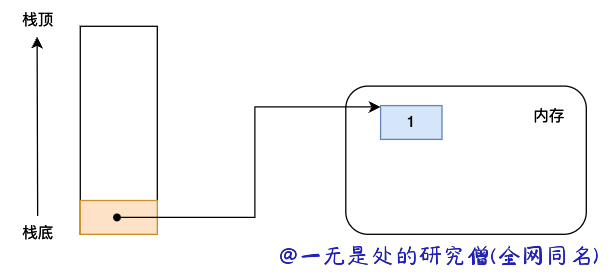
\includegraphics[scale=.2]{images/39-codeobject.png}
						\caption{ }
        \label{fig:my_label}
    \end{figure}
    
\item STORE\_FAST,将栈顶元素弹出并且保存到 co\_varnames 对应的下标当中,根据上面的字节码参数等于 0 ,因此将 1 保存到 co\_varnames[0] 对应的对象当中。 

    \begin{figure}[H]
        \centering
            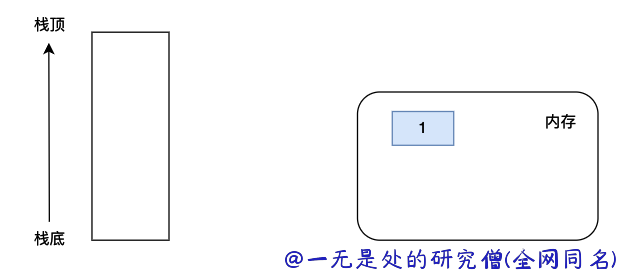
\includegraphics[scale=.2]{images/40-codeobject.png}
						\caption{ }
        \label{fig:my_label}
    \end{figure}
    
\item LOAD\_CONST,将下标等于 2 的常量加载进入栈中。 

    \begin{figure}[H]
        \centering
            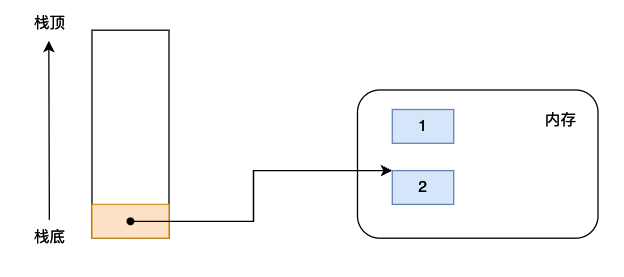
\includegraphics[scale=.2]{images/41-codeobject.png}
						\caption{ }
        \label{fig:my_label}
    \end{figure}
    
\item STORE\_FAST,将栈顶元素弹出,并且保存到 varnames 下标为 1 的对象。 

    \begin{figure}[H]
        \centering
            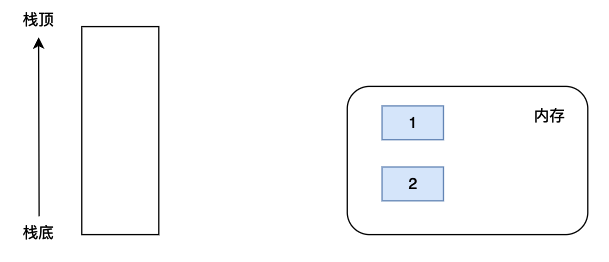
\includegraphics[scale=.2]{images/42-codeobject.png}
						\caption{ }
        \label{fig:my_label}
    \end{figure}
    
\item LOAD\_FAST,是取出 co\_varnames 对应下标的数据,并且将其压入栈中。我们直接连续执行两个 LOAD\_FAST 之后栈空间的布局如下: 

    \begin{figure}[H]
        \centering
            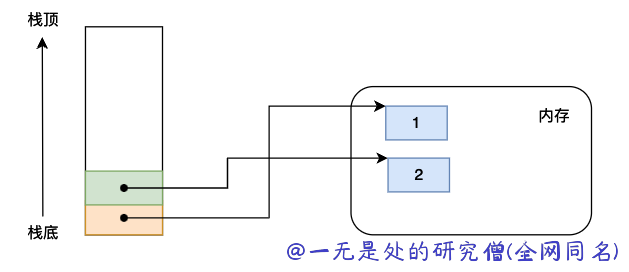
\includegraphics[scale=.2]{images/43-codeobject.png}
						\caption{ }
        \label{fig:my_label}
    \end{figure}
    
\item BINARY\_ADD,这个字节码指令是将栈空间的两个栈顶元素弹出,然后将两个数据进行相加操作,然后将相加得到的结果重新压入栈中。 

    \begin{figure}[H]
        \centering
            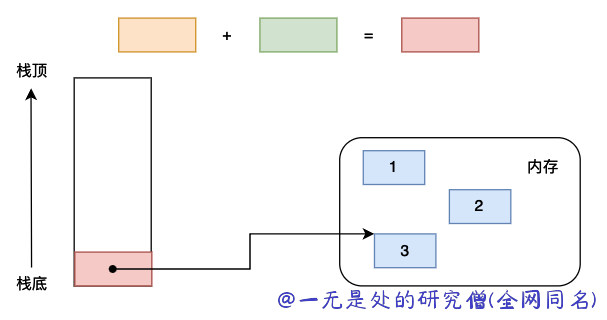
\includegraphics[scale=.2]{images/44-codeobject.png}
						\caption{ }
        \label{fig:my_label}
    \end{figure}
    
\item RETURN\_VALUE,将栈顶元素弹出并且作为返回值返回。 
\end{itemize}
从上面的整个执行过程来看整个栈空间使用的最大的空间长度为 2 ,因此 stacksize = 2 。
\subsection{总结}
在本小节当中主要分析了一些 code obejct 当中比较重要的字段,code object 是 cpython 虚拟机当中一个比较重要的数据结构,深入的去理解这里面的字段对于我们理解 python 虚拟机非常有帮助。

\section{深入理解 python 虚拟机:令人拍案叫绝的字节码设计}
在本小节当中主要给大家介绍 cpython 虚拟机对于字节码的设计以及在调试过程当中一个比较重要的字段 co\_lnotab 的设计原理!
\subsection{python 字节码设计}
一条 python 字节码主要有两部分组成,一部分是操作码,一部分是这个操作码的参数,在 cpython 当中只有部分字节码有参数,如果对应的字节码没有参数,那么 oparg 的值就等于 0 ,在 cpython 当中 opcode < 90 的指令是没有参数的。

    \begin{figure}[H]
        \centering
            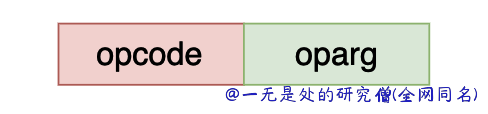
\includegraphics[scale=.25]{images/45-bytecode.png}
						\caption{ }
        \label{fig:my_label}
    \end{figure}

opcode 和 oparg 各占一个字节,cpython 虚拟机使用小端方式保存字节码。
我们使用下面的代码片段先了解一下字节码的设计:
\begin{lstlisting}[style=py,caption=, language=Python]

import dis
def add(a, b):
    return a + b
if __name__ == '__main__':
    print(add.__code__.co_code)
    print("bytecode: ", list(bytearray(add.__code__.co_code)))
    dis.dis(add)
\end{lstlisting}
上面的代码在 python3.9 的输出如下所示:
\begin{lstlisting}[style=cpp,caption=, language=C++]

b'|\x00|\x01\x17\x00S\x00'
bytecode:  [124, 0, 124, 1, 23, 0, 83, 0]
  5           0 LOAD_FAST                0 (a)
              2 LOAD_FAST                1 (b)
              4 BINARY_ADD
              6 RETURN_VALUE
\end{lstlisting}
首先 需要了解的是 \verb|add.__code__.co_code| 是函数 add 的字节码,是一个字节序列,\verb|list(bytearray(add.__code__.co_code))| 是将和这个序列一个字节一个字节进行分开,并且将其变成 10 进制形式。根据前面我们谈到的每一条指令——字节码占用 2 个字节,因此上面的字节码有四条指令:

    \begin{figure}[H]
        \centering
            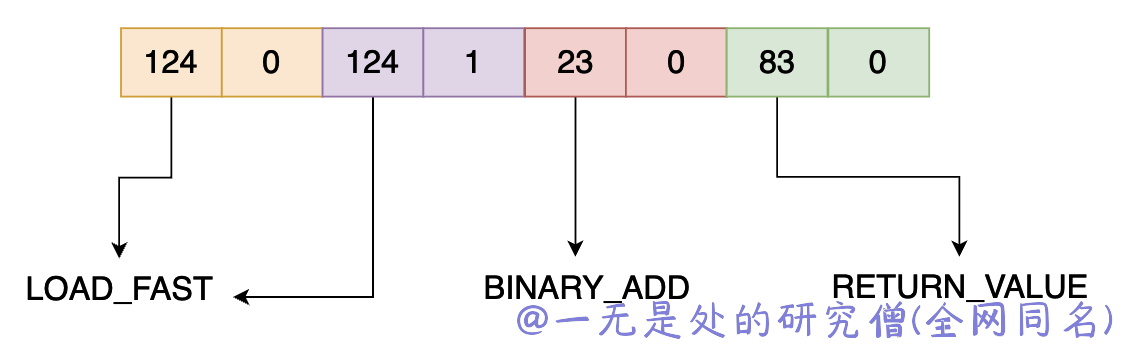
\includegraphics[scale=.25]{images/46-bytecode.png}
						\caption{ }
        \label{fig:my_label}
    \end{figure}

操作码和对应的操作指令在文末有详细的对应表。在上面的代码当中主要使用到了三个字节码指令分别是 124,23 和 83 ,他们对应的操作指令分别为 LOAD\_FAST,BINARY\_ADD,RETURN\_VALUE。他们的含义如下:
\begin{itemize}
\item LOAD\_FAST:将 varnames[var\_num] 压入栈顶。
\item BINARY\_ADD:从栈中弹出两个对象并且将它们相加的结果压入栈顶。
\item RETURN\_VALUE:弹出栈顶的元素,将其作为函数的返回值。
\end{itemize}
首先我们需要知道的是 BINARY\_ADD 和 RETURN\_VALUE,这两个操作指令是没有参数的,因此在这两个操作码之后的参数都是 0 。
但是 LOAD\_FAST 是有参数的,在上面我们已经知道 LOAD\_FAST 是将 co-varnames[var\_num] 压入栈,var\_num 就是指令 LOAD\_FAST 的参数。在上面的代码当中一共有两条 LOAD\_FAST 指令,分别是将 a 和 b 压入到栈中,他们在 varnames 当中的下标分别是 0 和 1,因此他们的操作数就是 0 和 1 。
\subsection{字节码扩展参数}
在上面我们谈到的 python 字节码操作数和操作码各占一个字节,但是如果 varnames 或者常量表的数据的个数大于 1 个字节的表示范围的话那么改如何处理呢?
为了解决这个问题,cpython 为字节码设计的扩展参数,比如说我们要加载常量表当中的下标为 66113 的对象,那么对应的字节码如下:
\begin{lstlisting}[style=py,caption=, language=Python]

[144, 1, 144, 2, 100, 65]
\end{lstlisting}
其中 144 表示 EXTENDED\_ARG,他本质上不是一个 python 虚拟机需要执行的字节码,这个字段设计出来主要是为了用与计算扩展参数的。
100 对应的操作指令是 LOAD\_CONST ,其操作码是 65,但是上面的指令并不会加载常量表当中下标为 65 对象,而是会加载下标为 66113 的对象,原因就是因为  EXTENDED\_ARG 。
现在来模拟一下上面的分析过程:
\begin{itemize}
\item 先读取一条字节码指令,操作码等于 144 ,说明是扩展参数,那么此时的参数 arg 就等于 (1 x (1 << 8)) = 256 。
\item 读取第二条字节码指令,操作码等于 144 ,说明是扩展参数,因为前面 arg 已经存在切不等于 0 了,那么此时 arg 的计算方式已经发生了改变,arg = arg << 8 + 2 << 8 ,也就是说原来的 arg 乘以 256 再加上新的操作数乘以 256 ,此时 arg = 66048 。
\item 读取第三条字节码指令,操作码等于 100,此时是 LOAD\_CONST 这条指令,那么此时的操作码等于 arg += 65,因为操作码不是 EXTENDED\_ARG 因此操作数不需要在乘以 256 了。
\end{itemize}
上面的计算过程用程序代码表示如下,下面的代码当中 code 就是真正的字节序列 HAVE\_ARGUMENT = 90 。
\begin{lstlisting}[style=py,caption=, language=Python]

def _unpack_opargs(code):
    extended_arg = 0
    for i in range(0, len(code), 2):
        op = code[i]
        if op >= HAVE_ARGUMENT:
            arg = code[i+1] | extended_arg
            extended_arg = (arg << 8) if op == EXTENDED_ARG else 0
        else:
            arg = None
        yield (i, op, arg)
\end{lstlisting}
我们可以使用代码来验证我们前面的分析:
\begin{lstlisting}[style=py,caption=, language=Python]

import dis
def num_to_byte(n):
    return n.to_bytes(1, "little")
def nums_to_bytes(data):
    ans = b"".join([num_to_byte(n) for n in data])
    return ans
if __name__ == '__main__':
    \section{extended_arg extended_num opcode oparg for python_version > 3.5}
    bytecode = nums_to_bytes([144, 1, 144, 2, 100, 65])
    print(bytecode)
    dis.dis(bytecode)
\end{lstlisting}
上面的代码输出结果如下所示:
\begin{lstlisting}[style=cpp,caption=, language=C++]

b'\x90\x01\x90\x02dA'
          0 EXTENDED_ARG             1
          2 EXTENDED_ARG           258
          4 LOAD_CONST           66113 (66113)
\end{lstlisting}
根据上面程序的输出结果可以看到我们的分析结果是正确的。
\subsection{源代码字节码映射表}
在本小节主要分析一个 code object 对象当中的 co\_lnotab 字段,通过分析一个具体的字段来学习这个字段的设计。
\begin{lstlisting}[style=py,caption=, language=Python]

import dis
def add(a, b):
    a += 1
    b += 2
    return a + b
if __name__ == '__main__':
    dis.dis(add.__code__)
    print(f"{list(bytearray(add.__code__.co_lnotab)) = }")
    print(f"{add.__code__.co_firstlineno = }")
\end{lstlisting}
首先 dis 的输出第一列是字节码对应的源代码的行号,第二列是字节码在字节序列当中的位移。
上面的代码输出结果如下所示:
\begin{lstlisting}[style=cpp,caption=, language=C++]

  源代码的行号  字节码的位移
  6           0 LOAD_FAST                0 (a)
              2 LOAD_CONST               1 (1)
              4 INPLACE_ADD
              6 STORE_FAST               0 (a)
  7           8 LOAD_FAST                1 (b)
             10 LOAD_CONST               2 (2)
             12 INPLACE_ADD
             14 STORE_FAST               1 (b)
  8          16 LOAD_FAST                0 (a)
             18 LOAD_FAST                1 (b)
             20 BINARY_ADD
             22 RETURN_VALUE
list(bytearray(add.__code__.co_lnotab)) = [0, 1, 8, 1, 8, 1]
add.__code__.co_firstlineno = 5
\end{lstlisting}
从上面代码的输出结果可以看出字节码一共分成三段,每段表示一行代码的字节码。现在我们来分析一下 co\_lnotab 这个字段,这个字段其实也是两个字节为一段的。比如上面的 [0, 1, 8, 1, 8, 1] 就可以分成三段 [0, 1], [8, 1], [8, 1] 。这其中的含义分别为:
\begin{itemize}
\item 第一个数字表示距离上一行代码的字节码数目。
\item 第二个数字表示距离上一行有效代码的行数。
\end{itemize}
现在我们来模拟上面代码的字节码的位移和源代码行数之间的关系:
\begin{itemize}
\item [0, 1],说明这行代码离上一行代码的字节位移是 0 ,因此我们可以看到使用 dis 输出的字节码 LOAD\_FAST ,前面的数字是 0,距离上一行代码的行数等于 1 ,代码的第一行的行号等于 5,因此 LOAD\_FAST 对应的行号等于 5 + 1 = 6 。
\item [8, 1],说明这行代码距离上一行代码的字节位移为 8 个字节,因此第二块的 LOAD\_FAST 前面是 8 ,距离上一行代码的行数等于 1,因此这个字节码对应的源代码的行号等于 6 + 1 = 7。
\item [8, 1],同理可以知道这块字节码对应源代码的行号是 8 。
\end{itemize}
现在有一个问题是当两行代码之间相距的行数超过 一个字节的表示范围怎么办?在 python3.5 以后如果行数差距大于 127,那么就使用 (0, 行数) 对下一个组合进行表示,(0, $x\_1$), (0,$ x\_2$) ... ,直到 $x\_1 + ... + x\_n$ = 行数。
在后面的程序当中我们会使用 compile 这个 python 内嵌函数。当你使用Python编写代码时,可以使用\verb|compile()|函数将Python代码编译成字节代码对象。这个字节码对象可以被传递给Python的解释器或虚拟机,以执行代码。
\verb|compile()|函数接受三个参数:
\begin{itemize}
\item \verb|source|: 要编译的Python代码,可以是字符串,字节码或AST对象。
\item \verb|filename|: 代码来源的文件名(如果有),通常为字符串。
\item \verb|mode|: 编译代码的模式。可以是 'exec'、'eval' 或 'single' 中的一个。'exec' 模式用于编译多行代码,'eval' 用于编译单个表达式,'single' 用于编译单行代码。
\end{itemize}
\begin{lstlisting}[style=py,caption=, language=Python]

import dis
code = """
x=1
y=2
""" \
+ "\n" * 500 + \
"""
z=x+y
"""
code = compile(code, '<string>', 'exec')
print(list(bytearray(code.co_lnotab)))
print(code.co_firstlineno)
dis.dis(code)
\end{lstlisting}
上面的代码输出结果如下所示:
\begin{lstlisting}[style=cpp,caption=, language=C++]

[0, 1, 4, 1, 4, 127, 0, 127, 0, 127, 0, 121]
1
  2           0 LOAD_CONST               0 (1)
              2 STORE_NAME               0 (x)
  3           4 LOAD_CONST               1 (2)
              6 STORE_NAME               1 (y)
505           8 LOAD_NAME                0 (x)
             10 LOAD_NAME                1 (y)
             12 BINARY_ADD
             14 STORE_NAME               2 (z)
             16 LOAD_CONST               2 (None)
             18 RETURN_VALUE
\end{lstlisting}
根据我们前面的分析因为第三行和第二行之间的差距大于 127 ,因此后面的多个组合都是用于表示行数的。
505 = 3(前面已经有三行了) + (127 + 127 + 127 + 121)(这个是第二行和第三行之间的差距,这个值为 502,中间有 500 个换行但是因为字符串相加的原因还增加了两个换行,因此一共是 502 个换行)。
具体的算法用代码表示如下所示,下面的参数就是我们传递给 dis 模块的 code,也就是一个 code object 对象。
\begin{lstlisting}[style=py,caption=, language=Python]

def findlinestarts(code):
    """Find the offsets in a byte code which are start of lines in the source.
    Generate pairs (offset, lineno) as described in Python/compile.c.
    """
    byte_increments = code.co_lnotab[0::2]
    line_increments = code.co_lnotab[1::2]
    bytecode_len = len(code.co_code)
    lastlineno = None
    lineno = code.co_firstlineno
    addr = 0
    for byte_incr, line_incr in zip(byte_increments, line_increments):
        if byte_incr:
            if lineno != lastlineno:
                yield (addr, lineno)
                lastlineno = lineno
            addr += byte_incr
            if addr >= bytecode_len:
                \section{The rest of the lnotab byte offsets are past the end of}
                \section{the bytecode, so the lines were optimized away.}
                return
        if line_incr >= 0x80:
            \section{line_increments is an array of 8-bit signed integers}
            line_incr -= 0x100
        lineno += line_incr
    if lineno != lastlineno:
        yield (addr, lineno)
\end{lstlisting}
\subsection{python 字节码表}
\begin{table}[H]
    \centering
    \caption{操作及操作码}
      \begin{tabular}{|l|l|}
      \hline
      操作    & 操作码 \\
      \hline
      POP\_TOP & 1 \\\hline
      ROT\_TWO & 2 \\\hline
      ROT\_THREE & 3 \\\hline
      DUP\_TOP & 4 \\\hline
      DUP\_TOP\_TWO & 5 \\\hline
      \end{tabular}
\end{table}

\subsection{总结}
在本小节当中主要给大家介绍了 cpython 当中对于字节码和源代码和字节码之间的映射关系的具体设计,这对于我们深入去理解 cpython 虚拟机的设计非常有帮助!
\backmatter % 后记部分

\chapter{后记}
写这本书就是一时兴起。

\end{document}
